% this file is encoded in utf-8
% v1.7

\documentclass[12pt, a4paper]{_environment_source/ntust_report} 

\usepackage{fontspec}                            %加這個就可以設定字體 
\usepackage{xeCJK}                               %讓中英文字體分開設置 
\setmainfont[Mapping=tex-text]{Times New Roman}  %設定主要字型,也就是英文字型 
\setCJKmainfont{標楷體}                          %設定中文字型 
% \setCJKmainfont{AR PL KaitiM Big5} 
\XeTeXlinebreaklocale "zh"         %這兩行一定要加,中文才能自動換行 
\XeTeXlinebreakskip = 0pt plus 1pt %這兩行一定要加,中文才能自動換行



% 除非校方修改了論文格式 (margins, header, footer, 浮水印)
% 或者需要增加所用的 LaTeX 套件,
% 或者要改預設中文字型、編碼
% 否則毋須修改本檔內容
% 論文撰寫,請修改以 my_  開頭檔名的各檔案



\usepackage{titletoc}
\usepackage[nospace]{cite}  % for smart citation
\usepackage{geometry}       % for easy margin settings
\usepackage{subfigure}      % for subfigure
\usepackage{multirow}
%\usepackage[dvipdfm]{graphicx}  % for graphic   using eps
%\usepackage{graphicx}  % for graphic   using eps

% Salmon edited. Support the landscape pages in a (mainly) portrait document.
\usepackage{pdflscape}
\usepackage{lscape}
\usepackage{caption}

% Salmon edited. Support the Chinese indent for the first line.
\usepackage{indentfirst}

% Salmon edited. Support the hyperlink reference.
% \usepackage[hidelinks]{hyperref}
\usepackage[hyphens]{url}
\Urlmuskip=0mu plus 1mu\relax

% Salmon edited. Support the long table to change pages.
\usepackage{longtable}
% Salmon edited. Specifying your column width with m{...}.
\usepackage{array}

%\usepackage{epstopdf} % 當使用pdflatex時打開,如使用latex則不需開啟,此功能為將xxx.eps 自動判讀為XXX.pdf

%\usepackage{subfig} 
% \usepackage{algorithmic}  %演算法使用
\usepackage{algorithm}

% Salmon edited. Support the pseudocode.
\usepackage{algpseudocode}
\renewcommand{\algorithmicrequire}{\textbf{Input:}}
\renewcommand{\algorithmicensure}{\textbf{Output:}}

%
% margins setting
\geometry{verbose,a4paper,tmargin=3.5cm,bmargin=2cm,lmargin=3cm,rmargin=3cm}
%
\usepackage{amsmath}  % 各式 AMS 數學功能
\usepackage{amssymb}  % 各式 AMS 數學符號
\usepackage{mathrsfs} % 草寫體數學符號,在數學模式裡用 \mathscr{E} 得草寫 E
\usepackage{listings} % 程式列表套件
%
% listing setting
\lstset{breaklines=true, % 過長的程式行可斷行
extendedchars=false,     % 中文處理不需要 extendedchars
texcl=true,              % 中文註解需要有 TeX 處理過的 comment line, 所以設成 true
comment=[l]\%\%,         % 以雙「百分號」做為程式中文註解的起頭標記,配合 MATLAB
basicstyle=\small,       % 小號字體, 約 10 pt 大小
commentstyle=\upshape,   % 預設是斜體字,會影響註解裏的英文,改用正體
%language=Octave         % 會將一些 octave 指令以粗體顯示
}

\usepackage{url} % 在文稿中引用網址,可以用 \url{http://www.ntust.edu.tw} 方式

% 插圖套件 graphicx
% 使用者工作流程是用 pdftex 還是 latex + dvipdfmx?
% 視情況而有不同的參數
% 這裡作自動判斷
% 參考自
% http://www.tex.ac.uk/cgi-bin/texfaq2html?label=ifpdf
%\newcommand\mydvipdfmxflow{dvipdfmx}
%\newcommand\mypdftexflow{pdftex}
%
%\ifx\pdfoutput\undefined
%  % not running pdftex
%  \usepackage[dvipdfm]{graphicx}
%  \newcommand\myworkflow{dvipdfmx}  % set the flag for hyperref
%\else
%  \ifx\pdfoutput\relax
%    % not running pdftex
%    \usepackage[dvipdfm]{graphicx}
%    \newcommand\myworkflow{dvipdfmx}  % set the flag
%  \else
%    % running pdftex, with...
%    \ifnum\pdfoutput>0
%      % ... PDF output
%      \usepackage[pdftex]{graphicx}
%      \newcommand\myworkflow{pdftex}  % set the flag
%    \else
%      %...DVI output
%      \usepackage[dvipdfm]{graphicx}
%      \newcommand\myworkflow{dvipdfmx}  % set the flag
%    \fi
%  \fi
%\fi

\usepackage{fancyhdr}  % 借用增強功能型 header 套件來擺放浮水印 
% (佔用了 central header)
% 不需要浮水印的使用者仍可利用此套件,產生所需的 header, footer
%
% 啟動 fancy header/footer 套件
\pagestyle{fancy}
\fancyhead{}  % reset left, central, right header to empty
\fancyfoot[C]{\thepage} %中間 footer 擺放頁碼
\renewcommand{\headrulewidth}{0pt} % header 的直線; 0pt 則無線

% 如果不需要任何浮水印,則請把下列介於 >>> 與 <<< 之間
% 的文字行關掉 (行首加上百分號)
%% 浮水印 >>> 
% 7/23
% %
% % this file is encoded in utf-8
% % v1.7
% % 如果浮水印不是全篇需要,請把下列介於 >>> 與 <<<
% % 的「全篇浮水印專用碼」關掉 (行首加百分號)
% % 參考自 Keith Reckdahl 寫的 "Using Imported Graphics in LATEX2e" (epslatex.pdf) p.39
% % 如果只有特定頁需要浮水印
% % 則依該頁屬性使用下列之一的命令 
% % 普通頁命令 \thispagestyle{WaterMarkPage}
% % plain 頁命令 \thispagestyle{PlainWaterMarkPage}
% % empty 頁命令 \thispagestyle{EmptyWaterMarkPage}


% % 將重複使用的浮水印章
% % 圖檔是 my_watermark.xxx
% % 副檔名可以不加,可以是 latex 系統能處裡的任何格式:pdf, gif, png, jpg, eps, ...
% % 某些圖檔格式在某些工作流程可能需要作前置處裡。
% % 例如,pdflatex 無法直接處理 eps 檔
% %  latex + dvipdfmx 無法直接處理 pdf, gif, png, jpg, 需要用 ebb 小工具程式
% %  對圖檔產生 .bb 對應檔。
% % old code
% %\newsavebox{\mywatermark}
% %\sbox{\mywatermark}{\includegraphics[keepaspectratio,%
% %height=0.8\textheight,%
% %width=0.8\textwidth]{my_watermark}}
% % new code
% \newsavebox{\mywatermark}
% %7/23
% \sbox{\mywatermark}{
\includegraphics[keepaspectratio,
% width=22.5cm]{watermark/ntust_watermark.pdf}}


% % 將 central header 擺放浮水印的巨集指令
% \newcommand{\PlaceWaterMark}{\fancyhead[C]{\setlength{\unitlength}{1in}%
% \begin{picture}(0,0)%
% %\put(-2.2,-6){\usebox{\mywatermark}}% old code
% \put(-4.5,-11.0){\usebox{\mywatermark}}% new code
% \end{picture}}%
% }

% \fancyhead{}  % reset left, central, right header to empty
% %% 如果不需整篇論文都要浮水印
% %% 則下面  >>> 與 <<< 之間的程式碼請關閉
% %% >>> 全篇浮水印

% \PlaceWaterMark  % 每一頁都有浮水印 (除了 plain、empty 頁以外)

% % 重新定義 plain 頁面
% % 每張 plain 頁面 (每一章的第一頁) 也加浮水印

% \fancypagestyle{plain}{%
% \fancyhead{}%
% \PlaceWaterMark%
% \fancyfoot{}%
% \fancyfoot[C]{\thepage}
% \renewcommand{\headrulewidth}{0pt}%
% \renewcommand{\footrulewidth}{0pt}%
% }
% %% <<< 全篇浮水印

% %% 如果只有一、兩頁需要有浮水印
% %% 可以在該頁 (有頁碼) 使用 \thispagestyle{WaterMarkPage}
% %% 此命令不影響原有的 header、footer
% \fancypagestyle{WaterMarkPage}{%
% \PlaceWaterMark%
% }

% %% 如果只有一、兩頁 plain 頁需要有浮水印 (如 摘要、自傳等)
% %% 可以在該頁 (有頁碼) 使用 \thispagestyle{PlainWaterMarkPage}
% %% 只有頁碼與浮水印,沒有其他的 header、footer
% %% 等同於 plain page style + water mark
% \fancypagestyle{PlainWaterMarkPage}{%
% \fancyhead{}%
% \PlaceWaterMark%
% \fancyfoot{}%
% \fancyfoot[C]{\thepage}
% \renewcommand{\headrulewidth}{0pt}%
% \renewcommand{\footrulewidth}{0pt}%
% }

% %% 如果只有一、兩頁 empty 頁需要有浮水印 (如封面、書名頁)
% %% 可以在該頁 (無頁碼) 使用 \thispagestyle{EmptyWaterMarkPage}
% %% 等同於 empty page style + water mark
% \fancypagestyle{EmptyWaterMarkPage}{%
% \fancyhead{}%
% \PlaceWaterMark%
% \fancyfoot{}%
% \renewcommand{\headrulewidth}{0pt}%
% \renewcommand{\footrulewidth}{0pt}%
% }

%% <<< 浮水印



% global page layout
% Salmon edited. Default is 1.4.
\newcommand{\mybaselinestretch}{1.4}                 % 行距 1.5 倍 + 20%, (約為 double space)
\renewcommand{\baselinestretch}{\mybaselinestretch}  % 論文行距預設值
\parskip=2ex     % 段落之間的間隔為兩個 x 的高度
\parindent=2em   % 段首內縮由 CJK 控制,所以這裡就設成不內縮
% \parindent=24Pt

%%%%%%%%%%%%%%%%%%%%%%%%%%%%%
%  end of preamble
%%%%%%%%%%%%%%%%%%%%%%%%%%%%%  %基本的環境設定  無需改變  

\begin{document}

	% 下列中文名詞的定義,如果以註解方式關閉取消,
% 則會以系統原先的預設值 (英文) 替代
% 名詞 \prechaptername 預設值為 Chapter
% 名詞 \postchaptername 預設值為空字串
% 名詞 \tablename 預設值為 Table
% 名詞 \figurename 預設值為 Figure

\renewcommand\prechaptername{第} % 出現在每一章的開頭的「第 x 章」
\renewcommand\postchaptername{章}
\renewcommand{\tablename}{表} % 在文章中 table caption 會以「表 x」表示
\renewcommand{\figurename}{圖} % 在文章中 figure caption 會以「圖 x」表示

% 下列中文名詞的定義,用於論文固定的各部分之命名 (出現於目錄與該頁標題)
\newcommand{\nameInnerCover}{教授推薦書}
\newcommand{\nameCommitteeForm}{論文口試委員審定書}
\newcommand{\nameCopyrightForm}{授權書}
\newcommand{\nameCabstract}{論文摘要}
\newcommand{\nameEabstract}{Abstract}
\newcommand{\nameAckn}{誌謝}
\newcommand{\nameToc}{目錄}
\newcommand{\nameLot}{表目錄}
\newcommand{\nameTof}{圖目錄}
\newcommand{\nameToa}{演算法目錄}
\newcommand{\nameSlist}{符號說明}
\newcommand{\nameRef}{參考文獻}
\newcommand{\nameVita}{自傳}
 %在此檔案處定義文章中的中文名詞

	%----------------------------------------------------------------------------------------------------------------------------------------------------------
	%%% 以下是載入前頁、本文、後頁
	% 此行請勿更動

	%----------------------------------------------------------------------------------------------------------------------------------------------------------
	% front matter 前頁
	% 包括封面、書名頁、中文摘要、英文摘要、誌謝、目錄、表目錄、圖目錄、符號說明
	% 在撰寫各章草稿時,可以把此部份「關掉」,以節省無謂的編譯時間。
	% 實際內容由
	%    my_names.tex, my_cabstract.tex, my_eabstract.tex, my_ackn.tex, my_symbols.tex
	% 決定
	% ntust_frontpages.tex 此檔只提供整體架構的定義,不需更動
	% 在撰寫各章草稿時,可以把此部份「關掉」,以節省無謂的編譯時間。
	
	%
% this file is encoded in utf-8
% v1.7
% do not change the content of this file
% unless the thesis layout rule is changed
% 無須修改本檔內容,除非校方修改了
% 封面、書名頁、中文摘要、英文摘要、誌謝、目錄、表目錄、圖目錄、符號說明
% 等頁之格式
% this file is encoded in utf-8
%v1.7

% make the line spacing in effect
\renewcommand{\baselinestretch}{\mybaselinestretch}
\large % it needs a font size changing command to be effective

% default variables definitions
% 注意!!此處只是預設值,不需更改此處
% 請更改 my_names.tex 內容
\newcommand\cTitle{論文題目}
\newcommand\eTitle{MY THESIS TITLE}
\newcommand\myCname{王鐵雄}
\newcommand\myEname{Aron Wang}
\newcommand\myStudentID{M9315048}
\newcommand\advisorCnameA{南宮明博士}
\newcommand\advisorEnameA{Dr.~Ming Nangong}
\newcommand\advisorCnameB{李斯坦博士}
\newcommand\advisorEnameB{Dr.~Stein Lee}
\newcommand\advisorCnameC{徐 石博士}
\newcommand\advisorEnameC{Dr.~Sean~Hsu}
\newcommand\univCname{國立台灣科技大學}
\newcommand\univEname{National Taiwan University of science and technology}
\newcommand\deptCname{光電工程研究所}
\newcommand\fulldeptEname{Graduate School of Electro-Optical Engineering}
\newcommand\deptEname{Electro-optical Engineering}
\newcommand\collEname{College of Engineering}
\newcommand\degreeCname{碩士}
\newcommand\degreeEname{Master of Science}
\newcommand\cYear{九十四}
\newcommand\cMonth{六}
\newcommand\cDay{十}
%\newcounter{eYear}
\newcommand\eYear{2006}
\newcommand\eMonth{June}
\newcommand\ePlace{Chungli, Taoyuan, Taiwan}


 % user's names; to replace those default variable definitions
%
% this file is encoded in utf-8
% v1.7
% 填入你的論文題目、姓名等資料
% 如果題目內有必須以數學模式表示的符號,請用 \mbox{} 包住數學模式,如下範例
% 如果中文名字是單名,與姓氏之間建議以全形空白填入,如下範例
% 英文名字中的稱謂,如 Prof. 以及 Dr.,其句點之後請以不斷行空白~代替一般空白,如下範例
% 如果你的指導教授沒有如預設的三位這麼多,則請把相對應的多餘教授的中文、英文名
%    的定義以空的大括號表示
%    如,\renewcommand\advisorCnameB{}
%          \renewcommand\advisorEnameB{}
%          \renewcommand\advisorCnameC{}
%          \renewcommand\advisorEnameC{}

% 論文題目 (中文)
\renewcommand\cTitle{%我的碩士論文題目 
以遊玩特徵為導向的程序化內容生成方法
}

% 論文題目 (英文)
\renewcommand\eTitle{%My Thesis Title  
Game Design Goal Oriented Approach for Procedural Content Generation
%My Thesis Title  \mbox{$\cal{H}_\infty$} and \mbox{Al$_x$Ga$_{1-x}$As}
}

% 我的姓名 (中文)
\renewcommand\myCname{王澤浩}

% 我的姓名 (英文)
\renewcommand\myEname{Ze-Hao Wang}

%我的學號
\renewcommand\myStudentID{M10415096}

% 指導教授A的姓名 (中文)
\renewcommand\advisorCnameA{戴文凱 博士}

% 指導教授A的姓名 (英文)
\renewcommand\advisorEnameA{Dr.~Wen-Kai Tai}

% 指導教授B的姓名 (中文)
\renewcommand\advisorCnameB{}

% 指導教授B的姓名 (英文)
\renewcommand\advisorEnameB{}

% 指導教授C的姓名 (中文)
\renewcommand\advisorCnameC{}

% 指導教授C的姓名 (英文)
\renewcommand\advisorEnameC{}

% 校名 (中文)
\renewcommand\univCname{國立台灣科技大學}

% 校名 (英文)
\renewcommand\univEname{National Taiwan University of science and technology}

% 系所名 (中文)
\renewcommand\deptCname{資~訊~工~程~系}

% 系所全名 (英文)
\renewcommand\fulldeptEname{Department of Computer Science and Information Engineering}

% 系所短名 (英文, 用於書名頁學位名領域)
%\renewcommand\deptEname{Electro-Optical Engineering}

% 學院英文名 (如無,則以空的大括號表示)
%\renewcommand\collEname{College of Electrical and Communication Engineering}

% 學位名 (中文)
\renewcommand\degreeCname{碩士學位}

% 學位名 (英文)
%\renewcommand\degreeEname{Master of Science}

% 口試年份 (中文、民國)
\renewcommand\cYear{一百零六}

% 口試月份 (中文)
\renewcommand\cMonth{七} 

% 口試月份 (中文)
\renewcommand\cDay{二十七} 

% 口試年份 (阿拉伯數字、西元)
%\renewcommand\eYear{2009} 

% 口試月份 (英文)
%\renewcommand\eMonth{July}

% 學校所在地 (英文)
%\renewcommand\ePlace{Taipei, Taiwan}

%畢業級別;用於書背列印;若無此需要可忽略
\newcommand\GraduationClass{105}

%%%%%%%%%%%%%%%%%%%%%%
\newcommand\itsempty{}
%%%%%%%%%%%%%%%%%%%%%%%%%%%%%%%
%       ntust cover 封面
%%%%%%%%%%%%%%%%%%%%%%%%%%%%%%%
%
\begin{titlepage}
% no page number
% next page will be page 1

% aligned to the center of the page
\begin{center}
% font size (relative to 12 pt):
% \large (14pt) < \Large (18pt) < \LARGE (20pt) < \huge (24pt)< \Huge (24 pt)
%



\begin{figure}[htbp]
	\begin{minipage}[b]{5cm} 
		\raggedright
		
\includegraphics[width=1.1in]{frontpages/ntust_logo.pdf}
		\label{fig:ntust_logo}
	\end{minipage}% 
	\begin{minipage}[b]{0.5\textwidth} 
	\centering
	\makebox[3cm][c]{\Huge{\univCname}}\\  %顯示中文校名
	\vspace{0.5cm}
	\makebox[3cm][c]{\Huge{\deptCname}}\\ %顯示中文系所名
	\vspace{0.5cm}
	\end{minipage}%
\\ 
\rule{16cm}{3pt}
\end{figure}
%\hfill


\vspace{1cm}
\makebox[6cm][s]{\textbf{\Huge{\degreeCname 論文}}}\\ %顯示論文種類 (中文)
%\makebox[8cm][s]{\textbf{\Huge{\degreeCname 論文(初稿)}}}\\ %顯示論文種類 (中文)
\vspace{1cm}
%
% Set the line spacing to single for the titles (to compress the lines)
\renewcommand{\baselinestretch}{1}   %行距 1 倍
%\large % it needs a font size changing command to be effective
\Large{\cTitle}\\  % 中文題目
%
\vspace{1cm}
%
\Large{\eTitle}\\ %英文題目
\vspace{5cm}
% \makebox is a text box with specified width;
% option s: stretch
% use \makebox to make sure
% 「研究生:」 與「指導教授:」occupy the same width
\hspace{4.5cm} \makebox[3cm][s]{\Large{研 究 生:}}
\Large{\myCname}  % 顯示作者中文名
\hfill \makebox[1cm][s]{}\\
%
\vspace{0.3cm}
\hspace{4.5cm} \makebox[3cm][s]{\Large{學號:}}
\Large{\myStudentID}  %顯示指導教授A中文名
\hfill \makebox[1cm][s]{}\\
%
\vspace{1cm}
\hspace{4.5cm} \makebox[3cm][s]{\Large{指導教授:}}
\Large{\advisorCnameA}  %顯示指導教授A中文名
\hfill \makebox[1cm][s]{}\\
%
% 判斷是否有共同指導的教授 B
\ifx \advisorCnameB  \itsempty
\relax % 沒有 B 教授,所以不佔版面,不印任何空白
\else
% 共同指導的教授 B
\hspace{4.5cm} \makebox[3cm][s]{}
\Large{\advisorCnameB}  %顯示指導教授B中文名
\hfill \makebox[1cm][s]{}\\
\fi
%
% 判斷是否有共同指導的教授 C
\ifx \advisorCnameC  \itsempty
\relax % 沒有 C 教授,所以不佔版面,不印任何空白
\else
% 共同指導的教授 C
\hspace{4.5cm} \makebox[3cm][s]{}
\Large{\advisorCnameC}  %顯示指導教授C中文名
\hfill \makebox[1cm][s]{}\\
\fi
%
\vfill
\makebox[10cm][s]{\Large{中華民國\cYear 年\cMonth 月\cDay 日}}%
%
\end{center}
% Resume the line spacing to the desired setting
\renewcommand{\baselinestretch}{\mybaselinestretch}   %恢復原設定
% it needs a font size changing command to be effective
% restore the font size to normal
\normalsize
\end{titlepage}
%%%%%%%%%%%%%%


%%%%%%%%%%%%%%%%%%%%%%%%%%%%%%%
%       延後公開申請書 
%%%%%%%%%%%%%%%%%%%%%%%%%%%%%%%


\includepdf[pages=-]{frontpages/FirstPage/FirstPage.pdf}


%%%%%%%%%%%%%%%%%%%%%%%%%%%%%%%
%       指導教授推薦書 
%%%%%%%%%%%%%%%%%%%%%%%%%%%%%%%
%
% insert the printed standard form when the thesis is ready to bind
% 在口試完成後,再將已簽名的推薦書放入以便裝訂
% create an entry in table of contents for 推薦書
% 目前送出空白頁
%\newpage{\thispagestyle{empty}\addcontentsline{toc}{chapter}{\nameInnerCover}\mbox{}\clearpage}%
%\newpage

% 判斷是否要浮水印?
\ifx\mywatermark\undefined 
  \thispagestyle{empty}  % 無頁碼、無 header (無浮水印)
\else
  \thispagestyle{EmptyWaterMarkPage} % 無頁碼、有浮水印
\fi

%%%%%%%%%%%%%%%%%%%%%%%%%%%%%%%%%%%%%%%%%%%%%%%%%%%%%%%%%%%%%%%
%%no page number
%% create an entry in table of contents for 書名頁
%\addcontentsline{toc}{chapter}{\nameInnerCover}
%
%
%% aligned to the center of the page
%\begin{center}
%% font size (relative to 12 pt):
%% \large (14pt) < \Large (18pt) < \LARGE (20pt) < \huge (24pt)< \Huge (24 pt)
%% Set the line spacing to single for the titles (to compress the lines)
%\renewcommand{\baselinestretch}{1}   %行距 1 倍
%% it needs a font size changing command to be effective
%%中文題目
%\Large{\cTitle}\\ %%%%%
%\vspace{1cm}
%% 英文題目
%\Large{\eTitle}\\ %%%%%
%%\vspace{1cm}
%\vfill
%% \makebox is a text box with specified width;
%% option s: stretch
%% use \makebox to make sure
%% 「研究生:」 與「指導教授:」occupy the same width
%\makebox[3cm][s]{\large{研 究 生:}}
%\makebox[3cm][l]{\large{\myCname}} %%%%%
%\hfill
%\makebox[2cm][s]{\large{Student: }}
%\makebox[5cm][l]{\large{\myEname}}\\ %%%%%
%%
%%\vspace{1cm}
%%
%\makebox[3cm][s]{\large{指導教授:}}
%\makebox[3cm][l]{\large{\advisorCnameA}} %%%%%
%\hfill
%\makebox[2cm][s]{\large{Advisor: }}
%\makebox[5cm][l]{\large{\advisorEnameA}}\\ %%%%%
%%
%% 判斷是否有共同指導的教授 B
%\ifx \advisorCnameB  \itsempty
%\relax % 沒有 B 教授,所以不佔版面,不印任何空白
%\else
%%共同指導的教授B
%\makebox[3cm][s]{}
%\makebox[3cm][l]{\large{\advisorCnameB}} %%%%%
%\hfill
%\makebox[2cm][s]{}
%\makebox[5cm][l]{\large{\advisorEnameB}}\\ %%%%%
%\fi
%%
%% 判斷是否有共同指導的教授 C
%\ifx \advisorCnameC  \itsempty
%\relax % 沒有 C 教授,所以不佔版面,不印任何空白
%\else
%%共同指導的教授C
%\makebox[3cm][s]{}
%\makebox[3cm][l]{\large{\advisorCnameC}} %%%%%
%\hfill
%\makebox[2cm][s]{}
%\makebox[5cm][l]{\large{\advisorEnameC}}\\ %%%%%
%\fi
%%
%% Resume the line spacing to the desired setting
%\renewcommand{\baselinestretch}{\mybaselinestretch}   %恢復原設定
%\large %it needs a font size changing command to be effective
%%
%\vfill
%\makebox[4cm][s]{\large{\univCname}}\\% 校名
%\makebox[6cm][s]{\large{\deptCname}}\\% 系所名
%\makebox[3cm][s]{\large{\degreeCname 論文}}\\% 學位名
%%
%%\vspace{1cm}
%\vfill
%\large{A Thesis}\\%
%\large{Submitted to }%
%%
%\large{\fulldeptEname}\\%系所全名 (英文)
%%
%%
%\ifx \collEname  \itsempty
%\relax % 沒有學院名 (英文),所以不佔版面,不印任何空白
%\else
%% 有學院名 (英文)
%\large{\collEname}\\% 學院名 (英文)
%\fi
%%
%\large{\univEname}\\%校名 (英文)
%%
%\large{in Partial Fulfillment of the Requirements}\\
%%
%\large{for the Degree of}\\
%%
%\large{\degreeEname}\\%學位名(英文)
%
%\large{in}\\
%%
%\large{\deptEname}\\%系所短名(英文;表明學位領域)
%%
%\large{\eMonth\ \eYear}\\%月、年 (英文)
%%
%\large{\ePlace}% 學校所在地 (英文)
%\vfill
%\large{中華民國}%
%\large{\cYear}% %%%%%
%\large{年}%
%\large{\cMonth}% %%%%%
%\large{月}\\
%\end{center}
%% restore the font size to normal
%\normalsize
%\clearpage


\includepdf[pages=-, angle=90]{frontpages/CommitteeForms/CommitteeForm-A.pdf}

%%%%%%%%%%%%%%%%%%%%%%%%%%%%%%%%%%%%%%%%%%%%%%%%%%%%%%%%%%%%%%%%%%%%%
%%%%%%%%%%%%%%%%%%%%%%%%%%%%%%%
%       論文口試委員審定書 (計頁碼,但不印頁碼) 
%%%%%%%%%%%%%%%%%%%%%%%%%%%%%%%
%
% insert the printed standard form when the thesis is ready to bind
% 在口試完成後,再將已簽名的審定書放入以便裝訂
% create an entry in table of contents for 審定書
% 目前送出空白頁

%\newpage{\thispagestyle{empty}\addcontentsline{toc}{chapter}{\nameCommitteeForm}\mbox{}\clearpage}%

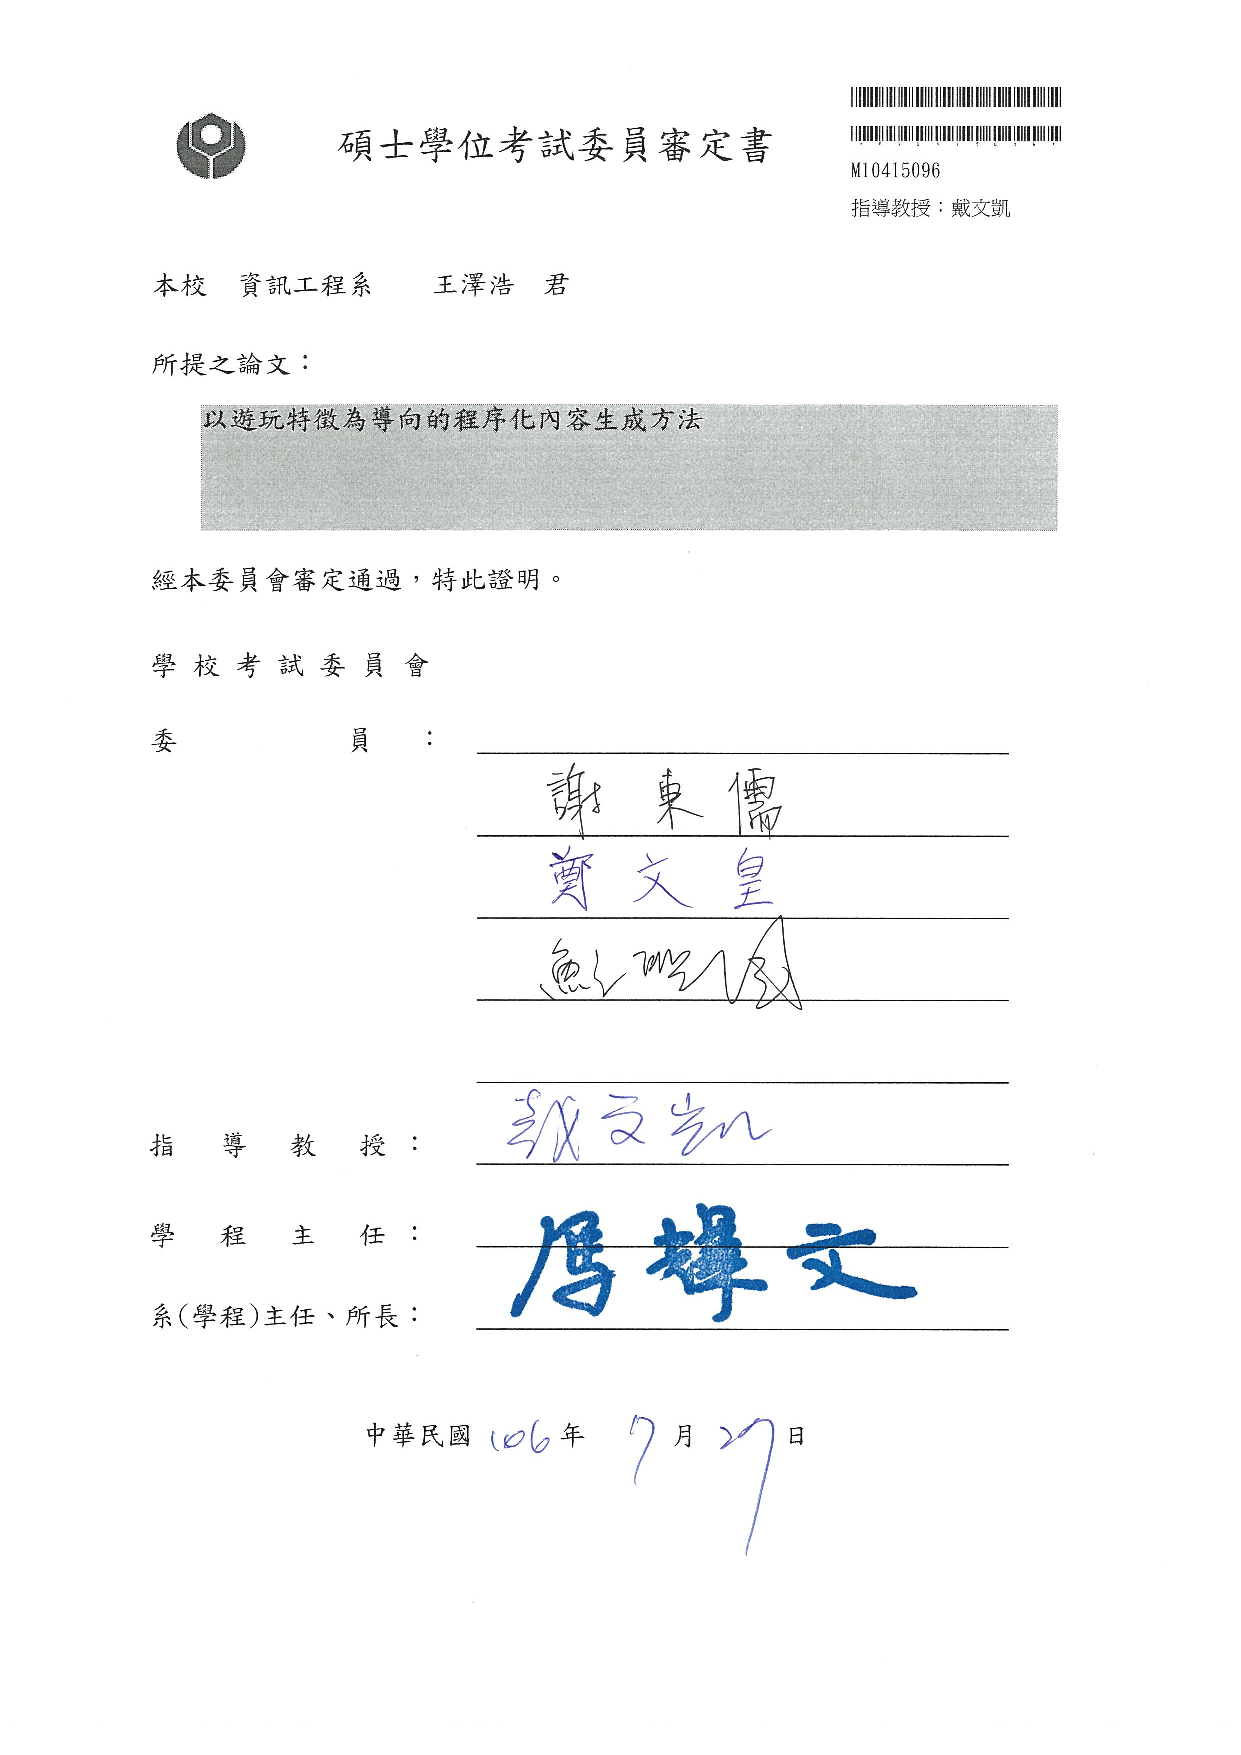
\includepdf[pages=-, angle=90]{frontpages/CommitteeForms/CommitteeForm-B.pdf}

%% 從摘要到本文之前的部份以小寫羅馬數字印頁碼
% 但是從「書名頁」(但不印頁碼) 就開始計算
%\setcounter{page}{1}
\pagenumbering{Roman}
%\pagenumbering{arabic}

%%%%%%%%%%%%%%%%%%%%%%%%%%%%%%%
%       中文摘要 
%%%%%%%%%%%%%%%%%%%%%%%%%%%%%%%
%
\newpage
\thispagestyle{plain}  % 無 header,但在浮水印模式下會有浮水印
% create an entry in table of contents for 中文摘要
\addcontentsline{toc}{chapter}{\nameCabstract}

% aligned to the center of the page
\begin{center}
% font size (relative to 12 pt):
% \large (14pt) < \Large (18pt) < \LARGE (20pt) < \huge (24pt)< \Huge (24 pt)
% Set the line spacing to single for the names (to compress the lines)
\renewcommand{\baselinestretch}{1}   %行距 1 倍
% it needs a font size changing command to be effective
%\large{\cTitle}\\  %中文題目
%\vspace{0.83cm}
% \makebox is a text box with specified width;
% option s: stretch
% use \makebox to make sure
% each text field occupies the same width
%\makebox[1.5cm][s]{\large{學生:}}
%\makebox[3cm][l]{\large{\myCname}} %學生中文姓名
%\hfill
%
%\makebox[3cm][s]{\large{指導教授:}}
%\makebox[3cm][l]{\large{\advisorCnameA}} \\ %教授A中文姓名
%
% 判斷是否有共同指導的教授 B
\ifx \advisorCnameB  \itsempty
\relax % 沒有 B 教授,所以不佔版面,不印任何空白
\else
%共同指導的教授B
\makebox[1.5cm][s]{}
\makebox[3cm][l]{} %%%%%
\hfill
\makebox[3cm][s]{}
\makebox[3cm][l]{\large{\advisorCnameB}}\\ %教授B中文姓名
\fi
%
% 判斷是否有共同指導的教授 C
\ifx \advisorCnameC  \itsempty
\relax % 沒有 C 教授,所以不佔版面,不印任何空白
\else
%共同指導的教授C
\makebox[1.5cm][s]{}
\makebox[3cm][l]{} %%%%%
\hfill
\makebox[3cm][s]{}
\makebox[3cm][l]{\large{\advisorCnameC}}\\ %教授C中文姓名
\fi
%
%\vspace{0.42cm} %2013/06/06
\vspace{0.38cm}
%
%\large{\univCname}\large{\deptCname}\\ %校名系所名
%\vspace{0.83cm}
%\vfill
\makebox[2.5cm][s]{\LARGE{中文摘要}}\\
\end{center}
% Resume the line spacing to the desired setting
\renewcommand{\baselinestretch}{\mybaselinestretch}   %恢復原設定
%it needs a font size changing command to be effective
% restore the font size to normal
\normalsize
%%%%%%%%%%%%%
  在本研究中,我們針對遊戲過程中的遊玩特徵 (gameplay patterns) 進行抽象化,使用程序化生成技術產生帶有意義遊戲關卡內容,藉此消彌或降低因隨機性所產生的不穩定要素,以改善並豐富遊戲體驗,最終提供一完整的遊戲關卡生成解決方案。

我們將「Mission/Space 框架」與「Multi-segment 演化」兩種關卡生成方法結合並予以改良,保留了前者追求的遊戲進程之順序性,後者帶來穩定且多樣化的遊戲內容,希冀藉此提升整體遊戲體驗、相輔相成。透過將遊戲關卡的劃分為任務 (Missions) 與空間 (Space) 兩種結構後,空間會依照任務結構進行有意義的同構轉換,並依照遊玩特徵定義基因演算法 (Genetic Algorithms) 的適應性函數。

利用此關卡生成解決方案來設計關卡能有效減少開發時間、容易掌握遊戲各元件的配置外,同時讓玩家在進行遊戲時能夠遵循關卡設計師的劇情脈絡,亦能夠體驗到有意義且多樣化的遊戲關卡內容。

關鍵字:關卡生成、程序化生成、基因演算法 

%%%%%%%%%%%%%%%%%%%%%%%%%%%%%%%
%       英文摘要 
%%%%%%%%%%%%%%%%%%%%%%%%%%%%%%%
%
\newpage
\thispagestyle{plain}  % 無 header,但在浮水印模式下會有浮水印

% create an entry in table of contents for 英文摘要
\addcontentsline{toc}{chapter}{\nameEabstract}

% aligned to the center of the page
\begin{center}
% font size:
% \large (14pt) < \Large (18pt) < \LARGE (20pt) < \huge (24pt)< \Huge (24 pt)
% Set the line spacing to single for the names (to compress the lines)
\renewcommand{\baselinestretch}{1}   %行距 1 倍
%\large % it needs a font size changing command to be effective
%\large{\eTitle}\\  %英文題目
%\vspace{0.83cm}
% \makebox is a text box with specified width;
% option s: stretch
% use \makebox to make sure
% each text field occupies the same width
%\makebox[2cm][s]{\large{Student: }}
%\makebox[5cm][l]{\large{\myEname}} %學生英文姓名
%\hfill
%
%\makebox[2cm][s]{\large{Advisor: }}
%\makebox[5cm][l]{\large{\advisorEnameA}} \\ %教授A英文姓名
%
% 判斷是否有共同指導的教授 B
\ifx \advisorCnameB  \itsempty
\relax % 沒有 B 教授,所以不佔版面,不印任何空白
\else
%共同指導的教授B
\makebox[2cm][s]{}
\makebox[5cm][l]{} %%%%%
\hfill
\makebox[2cm][s]{}
\makebox[5cm][l]{\large{\advisorEnameB}}\\ %教授B英文姓名
\fi
%
% 判斷是否有共同指導的教授 C
\ifx \advisorCnameC  \itsempty
\relax % 沒有 C 教授,所以不佔版面,不印任何空白
\else
%共同指導的教授C
\makebox[2cm][s]{}
\makebox[5cm][l]{} %%%%%
\hfill
\makebox[2cm][s]{}
\makebox[5cm][l]{\large{\advisorEnameC}}\\ %教授C英文姓名
\fi
%
%\vspace{0.42cm}
%\large{Submitted to }\large{\fulldeptEname}\\  %英文系所全名
%
\ifx \collEname  \itsempty
\relax % 如果沒有學院名 (英文),則不佔版面,不印任何空白
\else
% 有學院名 (英文)
%\large{\collEname}\\% 學院名 (英文)
\fi
%
%\large{\univEname}\\  %英文校名
%\vspace{0.83cm}
%\vfill
%
\large{ABSTRACT}\\
%\vspace{0.5cm}
\end{center}
% Resume the line spacing the desired setting
\renewcommand{\baselinestretch}{\mybaselinestretch}   %恢復原設定
%\large %it needs a font size changing command to be effective
% restore the font size to normal
\normalsize
%%%%%%%%%%%%%

	Ab. Under construction.

%%%%%%%%%%%%%%%%%%%%%%%%%%%%%%%
%       誌謝 
%%%%%%%%%%%%%%%%%%%%%%%%%%%%%%%
%
% Acknowledgment
\newpage
\chapter*{\protect\makebox[5cm][s]{\nameAckn}} %\makebox{} is fragile; need protect

\addcontentsline{toc}{chapter}{\nameAckn}
大家好,我是鄒濬安!!

%%%%%%%%%%%%%%%%%%%%%%%%%%%%%%%
%       目錄 
%%%%%%%%%%%%%%%%%%%%%%%%%%%%%%%
%
% Table of contents

\newpage

\renewcommand{\baselinestretch}{0.75}\normalsize

\renewcommand{\contentsname}{\protect\makebox[5cm][s]{\nameToc}}
%\makebox{} is fragile; need protect
\addcontentsline{toc}{chapter}{\nameToc}
\tableofcontents

\renewcommand{\baselinestretch}{\mybaselinestretch}\normalsize   %恢復原設定


%%%%%%%%%%%%%%%%%%%%%%%%%%%%%%%
%       圖目錄 
%%%%%%%%%%%%%%%%%%%%%%%%%%%%%%%
%
% List of Figures
\newcommand{\loflabel}{圖}
\newpage

\renewcommand{\baselinestretch}{0.75}\normalsize

\renewcommand{\numberline}[1]{\loflabel~#1\hspace*{1em}}
\renewcommand{\listfigurename}{\protect\makebox[5cm][s]{\nameTof}}
%\makebox{} is fragile; need protect
\addcontentsline{toc}{chapter}{\nameTof}
\listoffigures

\renewcommand{\baselinestretch}{\mybaselinestretch}\normalsize   %恢復原設定

%%%%%%%%%%%%%%%%%%%%%%%%%%%%%%%
%       表目錄 
%%%%%%%%%%%%%%%%%%%%%%%%%%%%%%%
%
% List of Tables
\newcommand{\lotlabel}{表}
\newpage

\renewcommand{\baselinestretch}{0.75}\normalsize

\renewcommand{\numberline}[1]{\lotlabel~#1\hspace*{1em}}
\renewcommand{\listtablename}{\protect\makebox[5cm][s]{\nameLot}}
%\makebox{} is fragile; need protect
\addcontentsline{toc}{chapter}{\nameLot}
\listoftables

\renewcommand{\baselinestretch}{\mybaselinestretch}\normalsize   %恢復原設定

%%%%%%%%%%%%%%%%%%%%%%%%%%%%%%%
%       演算法目錄 
%%%%%%%%%%%%%%%%%%%%%%%%%%%%%%%
%
% List of Figures
\newcommand{\loalabel}{演算法}
\newpage

\renewcommand{\baselinestretch}{1.5}\normalsize

\renewcommand{\numberline}[1]{\loalabel~#1\hspace*{1em}}
\renewcommand{\listalgorithmname}{\protect\makebox[5cm][s]{\nameToa}}
% \makebox{} is fragile; need protect
\addcontentsline{toc}{chapter}{\nameToa}
\listofalgorithms

\renewcommand{\baselinestretch}{\mybaselinestretch}\normalsize   %恢復原設定

%%%%%%%%%%%%%%%%%%%%%%%%%%%%%%%
%       符號說明 
%%%%%%%%%%%%%%%%%%%%%%%%%%%%%%%
%
% Symbol list
% define new environment, based on standard description environment
% adapted from p.60~64, <<The LaTeX Companion>>, 1994, ISBN 0-201-54199-8
%\newcommand{\SymEntryLabel}[1]%
% {\makebox[3cm][l]{#1}}
%
%\newenvironment{SymEntry}
%   {\begin{list}{}%
%       {\renewcommand{\makelabel}{\SymEntryLabel}%
%        \setlength{\labelwidth}{3cm}%
%        \setlength{\leftmargin}{\labelwidth}%
%        }%
%   }%
%   {\end{list}}
%%
%\newpage
%\chapter*{\protect\makebox[5cm][s]{\nameSlist}} %\makebox{} is fragile; need protect
%\addcontentsline{toc}{chapter}{\nameSlist}
%%
% this file is encoded in utf-8
% v1.7
%  各符號以 \item[] 包住,然後接著寫說明
% 如果符號是數學符號,應以數學模式表示,以取得正確的字體
% 如果符號本身帶有方括號,則此符號可以用大括號 {} 包住保護
\begin{SymEntry}

\item[OLED]
Organic Light Emitting Diode

\item[$E$]
energy

\item[$e$]
the absolute value of the electron charge, $1.60\times10^{-19}\,\text{C}$
 
\item[$\mathscr{E}$]
electric field strength (V/cm)

\item[{$A[i,j]$}]
the  element of the matrix $A$ at $i$-th row, $j$-th column\\
矩陣 $A$ 的第 $i$ 列,第 $j$ 行的元素

\end{SymEntry}


\newpage
\setcounter{page}{1}
\pagenumbering{arabic}
%% 論文本體頁碼回復為阿拉伯數字計頁,並從頭起算
%\pagenumbering{arabic}
%%%%%%%%%%%%%%%%%%%%%%%%%%%%%%%% 




	%----------------------------------------------------------------------------------------------------------------------------------------------------------
	% main body 論文主體。建議以「章」為檔案分割的依據。
	% 以下為建議的命名分類
	%   introduction.tex   related_work.tex  protocol.tex  evaluation.tex  conclusion.tex
	% 做為這幾個「章」的檔案名稱,並將檔案存放於資料夾 sections/ 下
	% 實際命名方式可以隨你意
	% 在撰寫各章草稿時,可以把其他章節關掉 (行首加百分號)
	%\input{example/example_body.tex}  % 所附的範例

	\chapter{緒論}
\label{cha:intro}

程序化內容生成 (Procedural Content Generation,以下簡稱 PCG) 在過去就廣泛被應用於遊戲設計領域,其主要目的為增加遊戲內容的隨機性與多樣性。在本研究中,我們針對遊戲過程中的遊玩特徵 (gameplay patterns) 進行抽象化,使用程序化生成技術產生帶有意義遊戲關卡內容,藉此消彌或降低因隨機性所產生的不穩定要素,以改善並豐富遊戲體驗。

我們將遊戲關卡的構成劃分為任務 (Missions) 與空間 (Space) 兩種結構後,空間會依照任務結構進行有意義的轉換,接著依照遊玩特徵定義基因演算法 (Genetic Algorithms) 的演化依據。讓玩家在進行遊戲時能夠遵循關卡設計師的劇情脈絡外,亦能夠體驗到有意義且多樣化的遊戲關卡內容。

\section{研究背景與動機}

在電腦圖學領域中,經常利用到 PCG 的技術來解決貼圖 (texture) 的生成、3D 模型的生成等。只需要運行的程式函數與基本的素材資源,便能夠藉由電腦快速運算出大量、豐富的內容,而這樣的特性相當適合被應用在電子遊戲領域中。PCG 遊戲開發技術已實行多年,採用相關技術開發的經典遊戲中,最早可追朔至由 Michael Toy 和 Glenn Wichman 於 1980 年左右開發的經典電子遊戲《\textit{Rogue}》,圖~\ref{fig:rogue-gameshot}。近年來,伴隨著遊戲產業的競爭下,成本的考量更加地重視,如涉及地圖場景、關卡設計的部分相當耗費人力成本。而 PCG 的遊戲開發技術,便是為了解決降低開發成本的同時保持遊戲性,甚至跳脫出人類的思考框架,進而創造出更豐富多樣的遊戲內容,因此這樣的技術又再度成為熱門焦點。

\begin{figure}[!htb]
  \begin{center}
    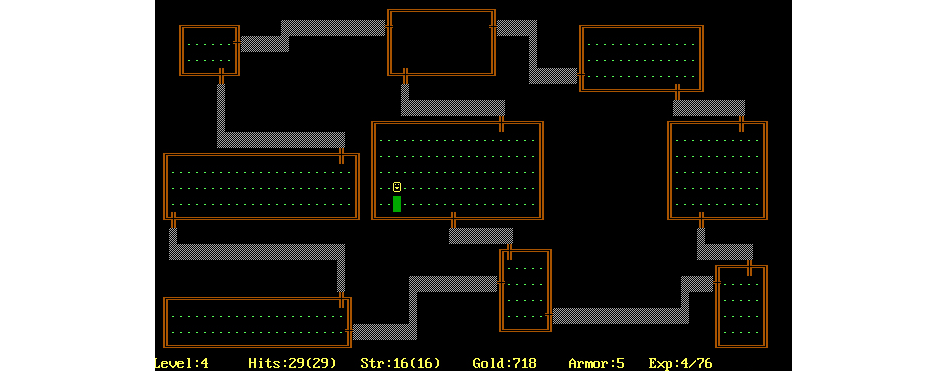
\includegraphics[width=1.0\textwidth]{figures/rogue-gameshot.png}
    \caption{Rogue 的遊戲畫面} 
    \label{fig:rogue-gameshot}
  \end{center}
\end{figure}

眾多開發團隊導入 PCG 技術至自家產品中,希冀藉此提升遊戲開發速度與其成本效益,不過目前的程序化生成技術還沒有辦法完全的取代人力。生成可遊玩的遊戲關卡是最低需求,僅以可遊玩為目標的話,現今已存在大量的程式與產品能夠達成此項目標。倘若需要兼顧內容品質與數量,那麼符合玩家遊戲體驗期待的 PCG 方法就顯得相當稀少,甚至只能針對特定的遊戲主題或產品。且隨機生成的內容是否能受玩家青睞與喜愛,仍是眾團隊需要研究的課題。

在本研究中,我們不涉及遊戲有趣程度的議題,緣由是受到遊戲本身的劇本主題、美術設計與關卡企劃等不同面向,因此我們把研究目標定位在如何藉由 PCG 技術,生成符合遊戲內容需求的地圖,藉由宏觀的抽象遊玩特徵,將其利用自動生成的方式實現出,並確保遊玩特徵的概念確實地落實在其生成結果當中。

% \subsection{迷宮探索遊戲 (dungeon crawl) 類型介紹}

% content here.

% \subsubsection{迷宮探索遊戲的歷史}

% content here.

\section{研究目的與研究問題}

由 Joris Dormans 提出的自動關卡設計方法中,藉由任務語法精準控制玩家遊玩的進程,而遊戲物件的佈局由空間語法掌控,卻無法控制其品質優劣。由 Antonios Liapis 提出的戰略型遊戲抽象化地圖生成方法中,對於遊戲物件的佈局提供了評定品質的量測方式,表~\ref{tbl:compare-the-method-form-jd-and-al} 對上述二者進行了簡易比較。

\begin{table}[!htb]
  \centering
  \caption{Joris Dormans 與 Antonios Liapis 提出之方法,進行綜觀比較}
  \label{tbl:compare-the-method-form-jd-and-al}
  \bigskip
  \begin{tabular}{ | c | c | c | }
    \hline
    方法框架                               & 任務進程 & 內容評估     \\\hline
    Mission/Space 框架(Joris Dormans)    & 精準控制 & 無法評估優劣 \\\hline
    Sentient Sketchbook(Antonios Liapis) & 未提及   & 提供優劣評估 \\\hline
  \end{tabular}
\end{table}

\subsection{研究目的}

我們將參考上一段落所提及的兩種方法框架,針對遊戲關卡的意義性與關卡品質進行研究。研究目的參照下列所述:

\begin{enumerate}
  \setlength\itemsep{-0.5em}
  \item 設計並提出能夠生成帶有意義的 3D 動作遊戲的關卡自動生成演算法。
  \item 以基因演算法輔助該自動生成演算法,進行自我品質評估與改良。
\end{enumerate}

\subsection{研究問題}

根據上述之研究目的,本研究提出以下研究問題:

\begin{enumerate}
  \setlength\itemsep{-0.5em}
  \item 存在多種不同面向的適應性函數,要如何進行有效的數值標準化?
  \item 人為調整相關基因演算法演化參數時,對於關卡生成會有什麼影響?
\end{enumerate}

\section{研究貢獻}

本論文提及之方法將進行整合與改良,最終提供關卡設計師一完整的遊戲關卡生成解決方案。並提出高度語意化的遊玩特徵指標,讓關卡設計師不須透過撰寫程式碼或設計數學模型,僅需調整各項遊玩指標的權重值便能生成出對應的複合型遊玩特徵。

\section{本論文之章節結構}

本論文第~\ref{cha:relatedworks} 章為相關研究,涵蓋了程序化生成技術應用於關卡生成之方法以及基因演算法。第~\ref{cha:methodology} 章為研究方法分為三節:其一,將巨觀的遊玩流程透過任務語法建立任務圖;其二,建構房間容器,並透過改寫系統將任務圖轉換為遊戲空間;其三,將關卡的各個房間容器,使用語意化的遊玩指標搭配基因演算法生成合適的遊戲物件佈局。第~\ref{cha:experiment} 章為實驗結果與分析,將呈現前述方法的系列實作結果,並且針對程序化生成的內容進行結果分析。第~\ref{cha:conclusions} 章為結論與後續工作,為本論文提出之方法及實作內容之結果進行總結,以及未來研究目標與其願景。
	\chapter{相關研究}
\label{cha:relatedworks}

本章劃分成四小節,第一節



\section{含有敘事脈絡的關卡}

content here.

content here.

content here.

\section{關卡生成 (Level Generation)}
\label{sec:relatedworks-levelgeneration}

本節收錄了至今的關卡生成框架與方法。而參考的文獻主要分為兩種類型,分別為~\ref{ssec:relatedworks-proceduralmission} 小節的程序化生成任務內容與~\ref{ssec:relatedworks-proceduralgamepatterns} 小節的程序化遊戲物件擺放。同時收錄數款採取關卡生成技術之遊戲。

\subsection{程序化生成任務內容}
\label{ssec:relatedworks-proceduralmission}

content here.

content here.

content here.

\subsubsection{Mission/Space 框架}
\label{sssec:relatedworks-proceduralmission-missionspace}

Joris Dormans 認為一個完整的關卡需要包含任務與空間二者~\cite{dormans2010adventures}~\cite{dormans2011level}~\cite{dormans2012engineering};需要有一特定的空間佈局,及一系列需要於此空間中被執行的任務。關卡任務代表玩家需要按照任務流程,來依序挑戰才能夠完成該關卡;關卡的空間由其地理佈局所組成,或者由與地圖相似的節點網絡所構成。由於任務與空間之間的交錯混雜,導致關卡設計者最終採取簡單卻有效的策略,也就是讓任務與空間同構。雖然同構在設計上不是唯一的選擇,但對於某些遊戲是非常合適的,特別是一具有線性的關卡設計。而 Joris Dormans 亦提出了一種自動關卡設計的方法~\cite{dormans2010adventures}~\cite{dormans2012engineering},藉由產生一個任務,再利用這個任務去產生適合此任務的空間。舉例來說,關卡設計者透過生成任務的介面來建立任務圖 (mission graph),玩家必須執行這些任務才能夠完成關卡,接下來將任務轉換為空間,並將任務依序安排至該空間圖 (space graph) 中。設計者接著在地圖添加更細節的內容,直到地圖充滿任務的要素並作為遊戲的關卡。

任務圖注重於任務與玩家的相互關係,表現出玩家距離通關的進度狀況。主要由兩種要件:節點和有向連結線所構成,其中節點再細分為任務、起點與終點;有向連結線再依照兩節點之間的執行先後關係,細分為薄弱條件、強烈條件與抑制。其中,強烈條件或抑制的關係,會導致某些節點無法執行。空間圖直接呈現了關卡的空間結構,且大多數的節點能夠直接表示出玩家目前所在位置。空間圖中的任何節點能透過顏色、字母來表示不同類型。主要亦由兩種要件:節點和連結線所構成。節點細分為場所、鎖和遊戲元素所構成;有向連結線細分為通道、閥、窗、解鎖與上鎖等。

改寫系統 (rewrite system) 由具有左側與右側的規則 (rules) 所組成,能夠將規則中指定的一符號集能夠被另一符號集所取代。改寫規則當中所使用的符號,便是在遊戲中經常會出現一些具有代表性的物件、要素或任務目標等,在字符表 (alphabet) 中定義以抽象化描述遊戲中的週期性結構 (recurrent construction)。改寫系統能夠套用在構成任務的圖形語法 (graph grammars) 及構成空間的形狀語法 (shape grammars),二者能夠獨立生成出結果,不過建議能夠將改寫系統套用在任務圖上,使其能夠產生出空間圖。本文提及之任務圖和空間圖是經過改良後的版本,定義其規則時會有些微上的不同,但更能夠體現出遊戲的關卡結構。

\subsubsection{Dungeon Crawl}
\label{sssec:relatedworks-proceduralmission-dungeoncrawl}

content here.

content here.

content here.

\subsubsection{遊戲 - Unexplored}
\label{sssec:relatedworks-proceduralmission-unexplored}

Unexplored 是由 ~\ref{sssec:relatedworks-proceduralmission-missionspace} 小節提及之框架作者 Joris Dormans 所製作,Joris Dormans 基於 Mission/Space 框架並提出改良的即時型戰鬥 roguelike 遊戲(若再細分可歸類於 roguelite 遊戲類型)。在市面上普遍的 roguelike 遊戲中,最常見的關卡生成策略即是視地下城玩家起點位置為樹之根,再以此根持續添加生成或預先設計的

Joris Dormans 稱改良後的方法為環狀地下城生成 (cyclic dungeon generation),在每一層的地牢中 ...

\subsection{程序化遊戲物件擺放}
\label{ssec:relatedworks-proceduralgamepatterns}

content here.

content here.

content here.

\subsubsection{Map Sketches 與 Segments 的演化}
\label{sssec:relatedworks-proceduralgamepatterns-mapsketches}

Antonios Liapis 開發了策略型遊戲的抽象化地圖生成工具 - Sentient Sketchbook~\cite{liapis2013generating}。在 Sentient Sketchbook 中,遊戲關卡設計師能夠以低分辯率、高階抽象的方式來編輯地圖草圖 (map sketches),構成地圖的瓦磚類型有資源磚、基地磚、不可通行磚與可通行磚等。典型的戰略型遊戲中,每位玩家都必須從隨機選擇的基地開始採集資源以建構戰鬥單位,並利用這些戰鬥單位摧毀敵方基地以完成遊戲。

當設計師編輯地圖時,該工具能夠測試地圖的可玩性 (意旨能夠正常進行遊戲) 且量化顯示,如果沒有足夠的基地、資源或可連通的路徑,那麼工具提供的遊玩特徵指標將會提示該地圖為不可遊玩的狀態。而這些遊玩特徵指標分別為資源安全性:距離基地僅一格以內的資源磚數量;安全區域:計算基地與敵方基地間的磚總數;探索性:利用洪水填充演算法,計算從基地至敵方基地時,可通行的磚總數。透過用戶當前編輯的地圖草圖,該工具利用基因演算法進行前述等指標,評估適應性函數 (fitness functions) 以解決約束最佳化 (constrained optimization) 等問題,來產生出更多意想不到的地圖輸出結果。

後續的研究中,Antonios Liapis 將基因演算法調整為兩階段演化,第一階段演化為地圖草圖演化,第二階段為地圖片段 (map segments) 演化~\cite{liapis2017multi}。地圖片段的結構類似於地圖草稿,由 NxN 的瓦磚所構成,瓦磚的種類能夠像是空磚、牆、連接處、出口、怪物或寶箱等,其中連接處是為了讓地圖片段彼此能夠接合以填滿地圖。利用地圖草稿所轉化成的初始地圖片段可作為演化用的胚胎 (embryogeny),於此階段定義的牆、連接處會呈顯穩定狀態,不隨著演化過程而改變,其餘瓦磚有機會由空磚突變為怪物、寶箱或牆,反之亦然。並探討不同的目標函數與胚胎,如何影響的圖片段的最佳解與外觀。

\begin{figure}[h]
  \begin{center}
    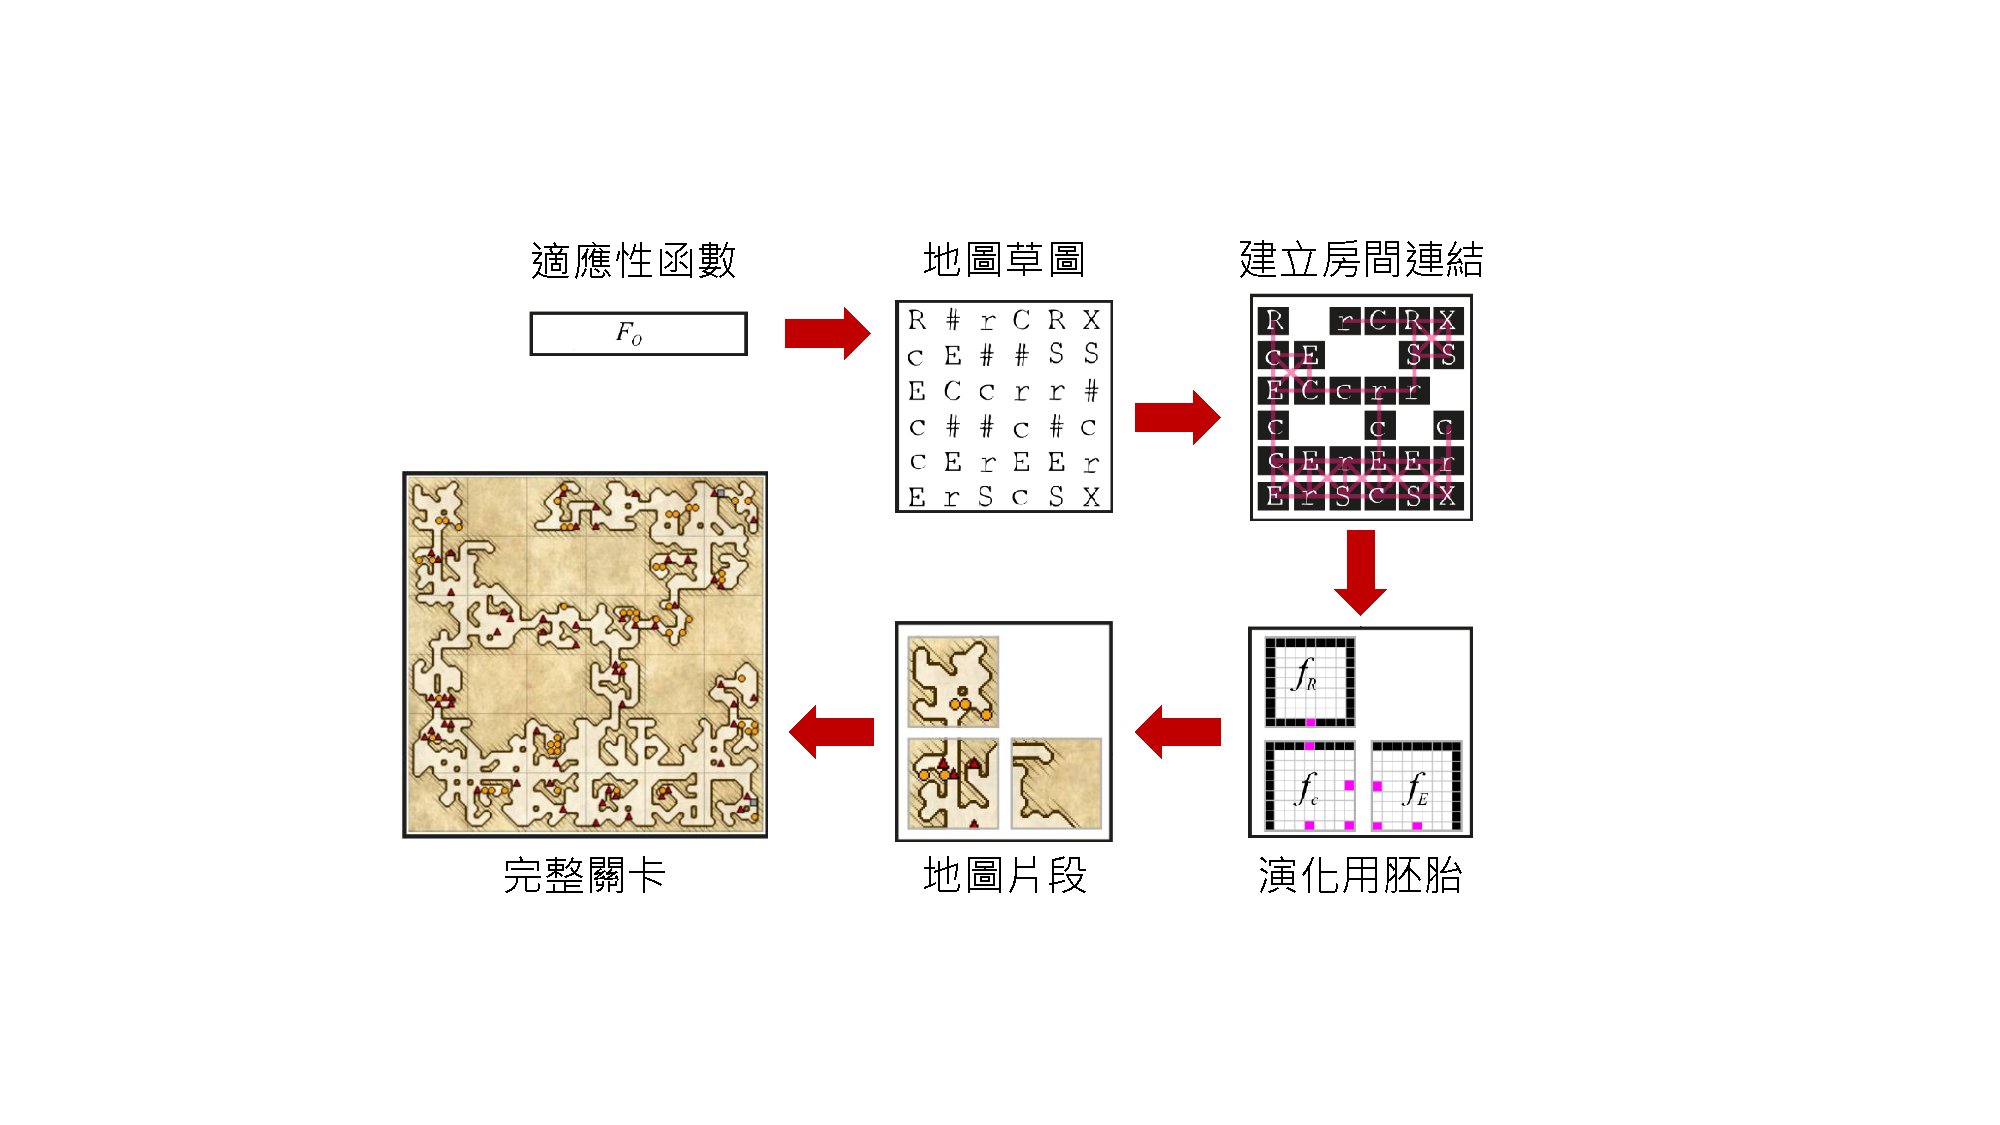
\includegraphics[width=1.0\textwidth]{figures/Multi-segment演化框架.pdf}
    \caption{Antonios Liaps 提出的兩階段式關卡演化。} 
    \label{fig:multi-segment-evolution}
  \end{center}
\end{figure}

\subsection{其它程序化生成技術}
\label{ssec:relatedworks-others}

content here.

content here.

content here.

\subsubsection{遊戲 - Spelunky}
\label{sssec:relatedworks-others-spelunky}

content here.

content here.

content here.

	% Quickly access the figures.
\newcommand{\missionalphabetnode}[2]{{\includegraphics[height=#2]{figures/mission-grammars-alphabet/#1.png}}}
\newcommand{\missioninstruction}[1]{{\begin{minipage}{.3\textwidth}\includegraphics[width=35mm]{figures/mission-grammars-ins-rep/#1.png}\end{minipage}}}

\chapter{研究方法}
\label{cha:methodology}

本論文中,我們仍保持 Joris Dormans~\cite{dormans2010adventures}~\cite{dormans2012engineering} 與 Antonios Liapis~\cite{liapis2013generating} 為求遊戲設計過程抽象化與高階化的訴求。將「Mission/Space 框架」與「Multi-segment 演化」兩種關卡生成方法結合並予以改良,保留了前者追求的遊戲進程之順序性,後者帶來穩定且多樣化的遊戲內容,希冀藉此提升整體遊戲體驗、相輔相成。

圖~\ref{fig:system-framework} 為系統的整體流程圖。遊戲設計師能夠透過宏觀的觀點來構築遊戲體驗流,將遊玩特徵拆分成多項規則,利用生成語法及改寫系統生成出任務圖 (mission graph),圖~\ref{fig:system-framework} a。依照任務圖中對應的終端節點 (terminal nodes) 轉換為事先建構完成的房間容器,並得到尚未包含遊戲物件的遊戲地圖,圖~\ref{fig:system-framework} b-c。接下來,針對動作冒險遊戲我們提出了數項評估遊戲性的適應性函數 (fitness functions),藉由基因演算法演化房間容器的流程,令各房間遵守適應性函數的限制,以得到符合訴求的最適解,圖~\ref{fig:system-framework} d-f。

\begin{figure}[!htb]
  \begin{center}
    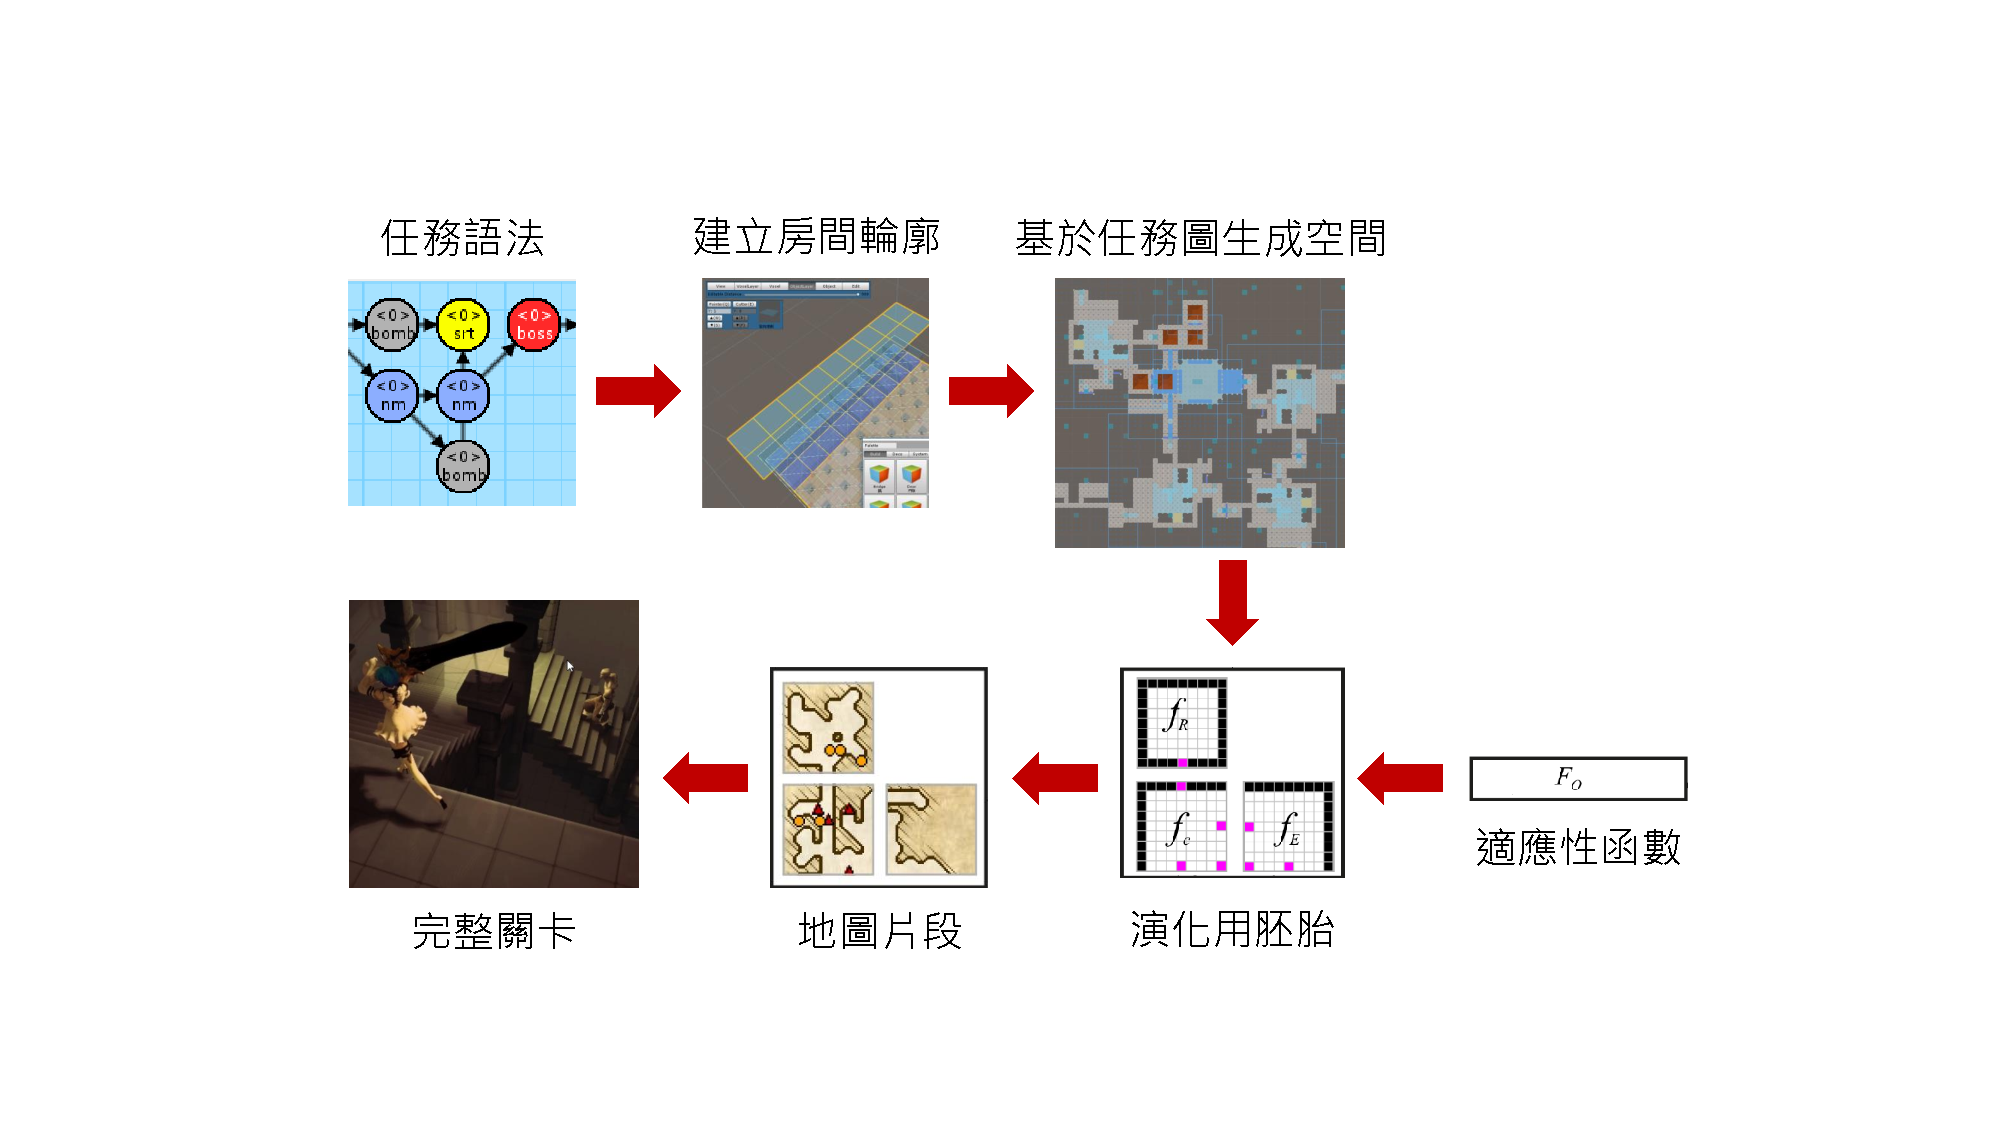
\includegraphics[width=1.0\textwidth]{figures/系統框架.png}
    \caption{本論文提出系統之流程圖} 
    \label{fig:system-framework}
  \end{center}
\end{figure}

\section{任務語法}
\label{sec:method-missiongrammars}

我們基於 Joris Dormans 提出之 Mission Grammars 概念,進行實作與改良出 \textit{Dungeon Generator} 工具。遊戲設計師能夠藉由 Dungeon Generator 工具進行任務語法的建置,並執行改寫系統以輸出任務圖,進一步利用任務圖產出遊戲關卡空間。

在任務語法的設計階段,我們參考~\ref{ssec:relatedworks-gameswithprocedural-isaac} 小節所提及之遊戲 \textit{The binding of Isaac} 的關卡地圖,分析其遊戲進程結構,構想期望的任務圖並將觀察其遊玩特徵,接著拆分成任務語法規則使用改寫規則產生出近似結構的任務圖。

\begin{figure}[!htb]
  \begin{center}
    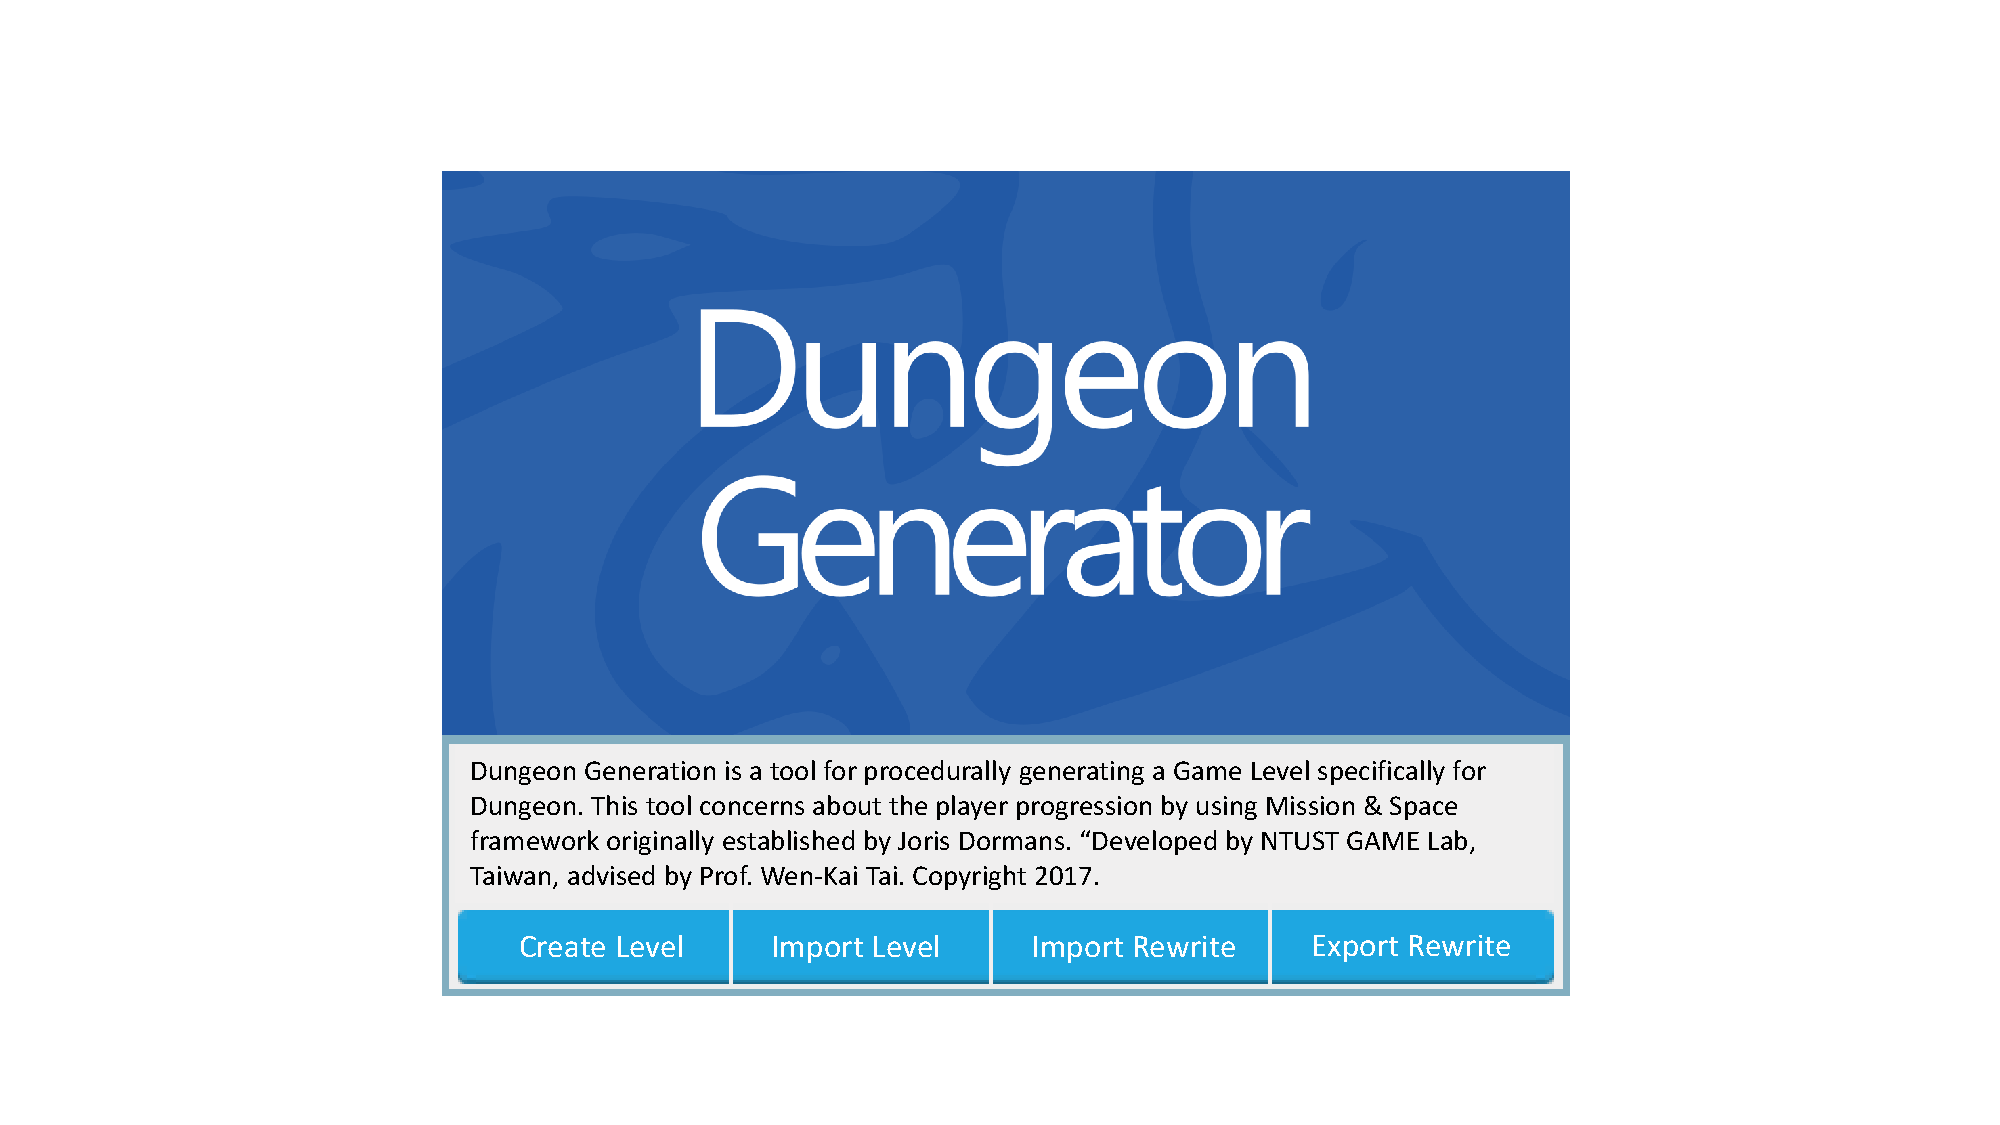
\includegraphics[width=1.0\textwidth]{figures/dungeon_generator.pdf}
    \caption{Dungeon Generator 工具} 
    \label{fig:dungeon-generator}
  \end{center}
\end{figure}

\subsection{建立任務符號表}
\label{ssec:method-missiongrammars-alphabet}

在本小節,會以 \textit{The binding of Isaac} 遊戲關卡作為範例,解析其遊玩特徵並作為任務語法的節點。表~\ref{tbl:mission-grammars-alphabet-default} 為系統預設任務符號表。

\begin{table}[!htb]
  \centering
  \caption{系統預設的任務符號}
  \label{tbl:mission-grammars-alphabet-default}
  \bigskip
  \begin{tabular}{
    | >{\centering\arraybackslash} m{2.8cm}
    | >{\centering\arraybackslash} m{2.0cm}
    | >{\centering\arraybackslash} m{1.0cm}
    | >{\arraybackslash} m{6.7cm} | }
    \hline
    \multicolumn{1}{ |c| }{代號}
      & \multicolumn{1}{ c| }{名稱}
      & \multicolumn{1}{ c| }{符號}
      & \multicolumn{1}{ c| }{說明} \\\hline
    ? (any)
      & 任一節點
      & \begin{minipage}{.3\textwidth}
\includegraphics[height=10mm]{figures/mission-grammars-alphabet/sys-any.png}\end{minipage}
      & 此節點無法修改,於~\ref{ssec:method-missiongrammars-rules} 小節 - 建立任務規則中,任一節點能夠被判別為任何節點,促使其同構。
      \\\hline
  \end{tabular}
\end{table}

\subsubsection{解析遊玩特徵}
\label{sssec:method-missiongrammars-alphabet-extractpatterns}

在任務語法中,任務節點可表示為一項事件、挑戰、動作或遊戲物件等。藉由觀察 \textit{The binding of Isaac} 的遊戲關卡後,能夠發現房間擁有固定類型,並且對於房間之間進行程序化的排列組合。然而固定的房間類型便是我們所尋找的節點種類,表~\ref{tbl:mission-grammars-alphabet} 將列舉利用遊玩特徵所建立的任務符號表,藉此歸納出「起點 (entrance\missionalphabetnode{t-entrance}{5mm})、終點 (goal\missionalphabetnode{t-goal}{5mm})、魔王房 (boss\missionalphabetnode{t-boss}{5mm})、一般房 (normal\missionalphabetnode{t-normal}{5mm})」外,以及一定機率會出現的稀有特殊房間「秘密房 (secret\missionalphabetnode{t-secret}{5mm})、商店 (shop\missionalphabetnode{t-shop}{5mm})、寶藏房 (treasure\missionalphabetnode{t-treasure}{5mm})」。這些稀有房間帶來了一些制式的事件,在進入秘密房前必須使用炸彈將牆壁給破壞的事件 (bomb\missionalphabetnode{t-bomb}{5mm}),以及從秘密房取得的鑰匙能夠進行解鎖 (lock\missionalphabetnode{t-lock}{5mm}),開通進入商店或寶藏房的權限。而前述的遊玩特徵將轉化為終端節點 (terminal nodes) 的圓形符號形式,表示較為詳盡的任務內容;另外一種為方形符號的非終端節點 (non-terminal nodes),相較於終端節點更為高階、抽象化,在此我們定義出起始節點 (Start\missionalphabetnode{nt-start}{5mm})、一般房 (Normal\missionalphabetnode{nt-normal}{5mm}) 與特殊房 (Special\missionalphabetnode{nt-special}{5mm}) 等,其應用方式將在下一小節~\ref{ssec:method-missiongrammars-rules} 中介紹。

\setlength\LTcapwidth{\linewidth}
\begin{longtable}{
    | >{\centering\arraybackslash} m{2.8cm}
    | >{\centering\arraybackslash} m{2.0cm}
    | >{\centering\arraybackslash} m{1.0cm}
    | >{\arraybackslash} m{4.7cm}
    | >{\centering\arraybackslash} m{2.0cm} | }
  \caption{利用遊玩特徵建立任務符號表之範例}\label{tbl:mission-grammars-alphabet} \\
  \hline
  代號 & 名稱 & 符號 & \multicolumn{1}{ c| }{說明} & 類型 \\
  \hline
  \endfirsthead
  \multicolumn{5}{c}%
  {\tablename\ \thetable\ -- \textit{接續前頁面}} \\
  \hline
  代號 & 名稱 & 符號 & \multicolumn{1}{ c| }{說明} & 類型 \\
  \hline
  \endhead
  \multicolumn{5}{r}{\textit{接續下頁面}} \\
  \endfoot
  \endlastfoot
  S (Start)
    & 起始節點
    & \missionalphabetnode{nt-start}{10mm}
    & 任務圖進入改寫階段時,系統預設的根節點。
    & 起始節點 \\\hline
  en (entrance)
    & 起點
    & \missionalphabetnode{t-entrance}{10mm}
    & 玩家於遊戲關卡開始時的起始位置。
    & \multirow{8.5}{*}{ 主線任務 } \\\cline{1-4}
    % 8.5 is special to centering.
  go (goal)
    & 終點
    & \missionalphabetnode{t-goal}{10mm}
    & 玩家抵達此位置時遊戲將結束。
    &  \\\cline{1-4}
  boss (boss)
    & 魔王房
    & \missionalphabetnode{t-boss}{10mm}
    & 房間中存在著較強大的怪物。
    &  \\\cline{1-4}
  NM (Normal)
    & 一般房
    & \missionalphabetnode{nt-normal}{10mm}
    & 一般房間,藉由其它規則替換成其它房間或事件。
    &  \\\cline{1-4}
  nm (normal)
    & 一般房
    & \missionalphabetnode{t-normal}{10mm}
    & 遊戲過程中經過的通道,經常出現在遊戲關卡中。
    &  \\\hline
  bomb (bomb)
    & 使用炸彈
    & \missionalphabetnode{t-bomb}{10mm}
    & 必須使用炸彈將石牆給破壞,破壞石牆後便可通過。
    & \multirow{10}{*}{ 特殊事件 } \\\cline{1-4}
    % 10 is special to centering.
  srt (secret)
    & 秘密房
    & \missionalphabetnode{t-secret}{10mm}
    & 能夠取得稀有道具鑰匙的房間。
    &  \\\cline{1-4}
  SP (Special)
    & 特殊房
    & \missionalphabetnode{nt-special}{10mm}
    & 特殊房間,藉由其它規則替換成不同的稀有房間。
    &  \\\cline{1-4}
  lock (lock)
    & 鎖
    & \missionalphabetnode{t-lock}{10mm}
    & 必須使用鑰匙才能夠通過該空間。
    &  \\\cline{1-4}
  shop (shop)
    & 商店
    & \missionalphabetnode{t-shop}{10mm}
    & 能夠觸發特殊事件,玩家能夠在此購買道具。
    &  \\\cline{1-4}
  ts (treasure)
    & 寶藏房
    & \missionalphabetnode{t-treasure}{10mm}
    & 藏有稀有道具的房間,當中會有守衛寶箱的敵人。
    &  \\\hline
\end{longtable}

% \subsubsection{任務符號表使用說明}
% \label{sssec:method-missiongrammars-alphabet-manual}

% content here.

% \begin{figure}[!htb]
%   \begin{center}
%     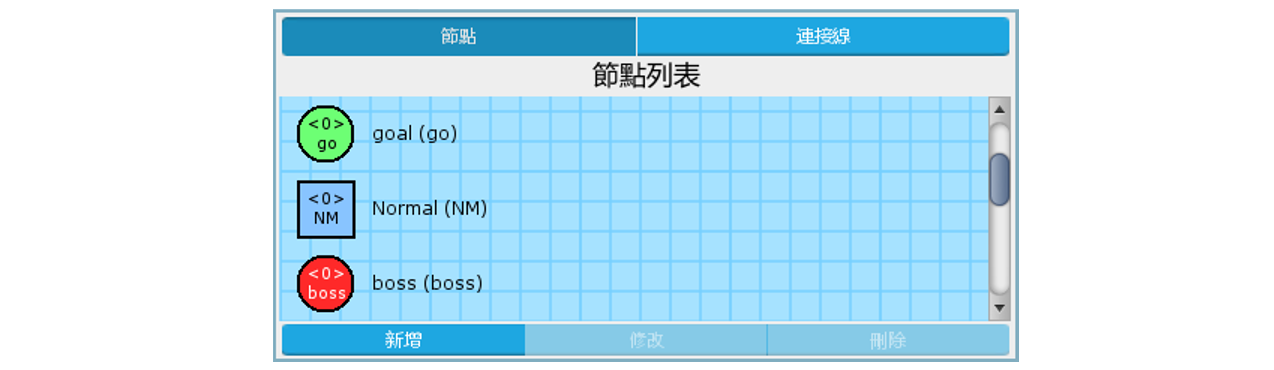
\includegraphics[width=1.0\textwidth]{figures/missiongrammars-alphabet-manual.png}
%     \caption{利用 Dungeon Generator 建立符號表} 
%     \label{fig:missiongrammars-alphabet-manual}
%   \end{center}
% \end{figure}

\subsection{建立任務規則}
\label{ssec:method-missiongrammars-rules}

圖~\ref{fig:missiongrammars-tutorial},任務規則分為規則左側及規則右側,二者皆為圖形語法 (Graph Grammars) 所構成,圖形與則由終端節點、非終端節點與連接線 (connection) 所構成的有向圖。規則左側為被取代方、規則右側為取代方,在任務圖中若有子圖符合任務規則的左側,將會依照流程進行替換改寫動作至規則右側,可參照第~\ref{ssec:method-missiongrammars-graph} 小節之說明。為了方便管理與分類不同性質的規則,在 \textit{Dungeon Generator} 中定義一任務語法包含了多個任務規則群組,各自群組底下有複數個任務改寫規則。規則被賦予使用數量上的條件限制,分為使用上限次數與下限次數,上限次數表示完整的改寫系統運行過程,最多能夠套用該規則的次數上限,多為了因應部分遊玩特徵的獨特性或稀有性;反之,下限次數表示套用該規則的次數下限,能用於改寫系統的疊代結果已趨於穩定、無剩餘任何非終端節點的情形下,作為持續進行改寫系統的強制約束條件。

\begin{figure}[!htb]
  \begin{center}
    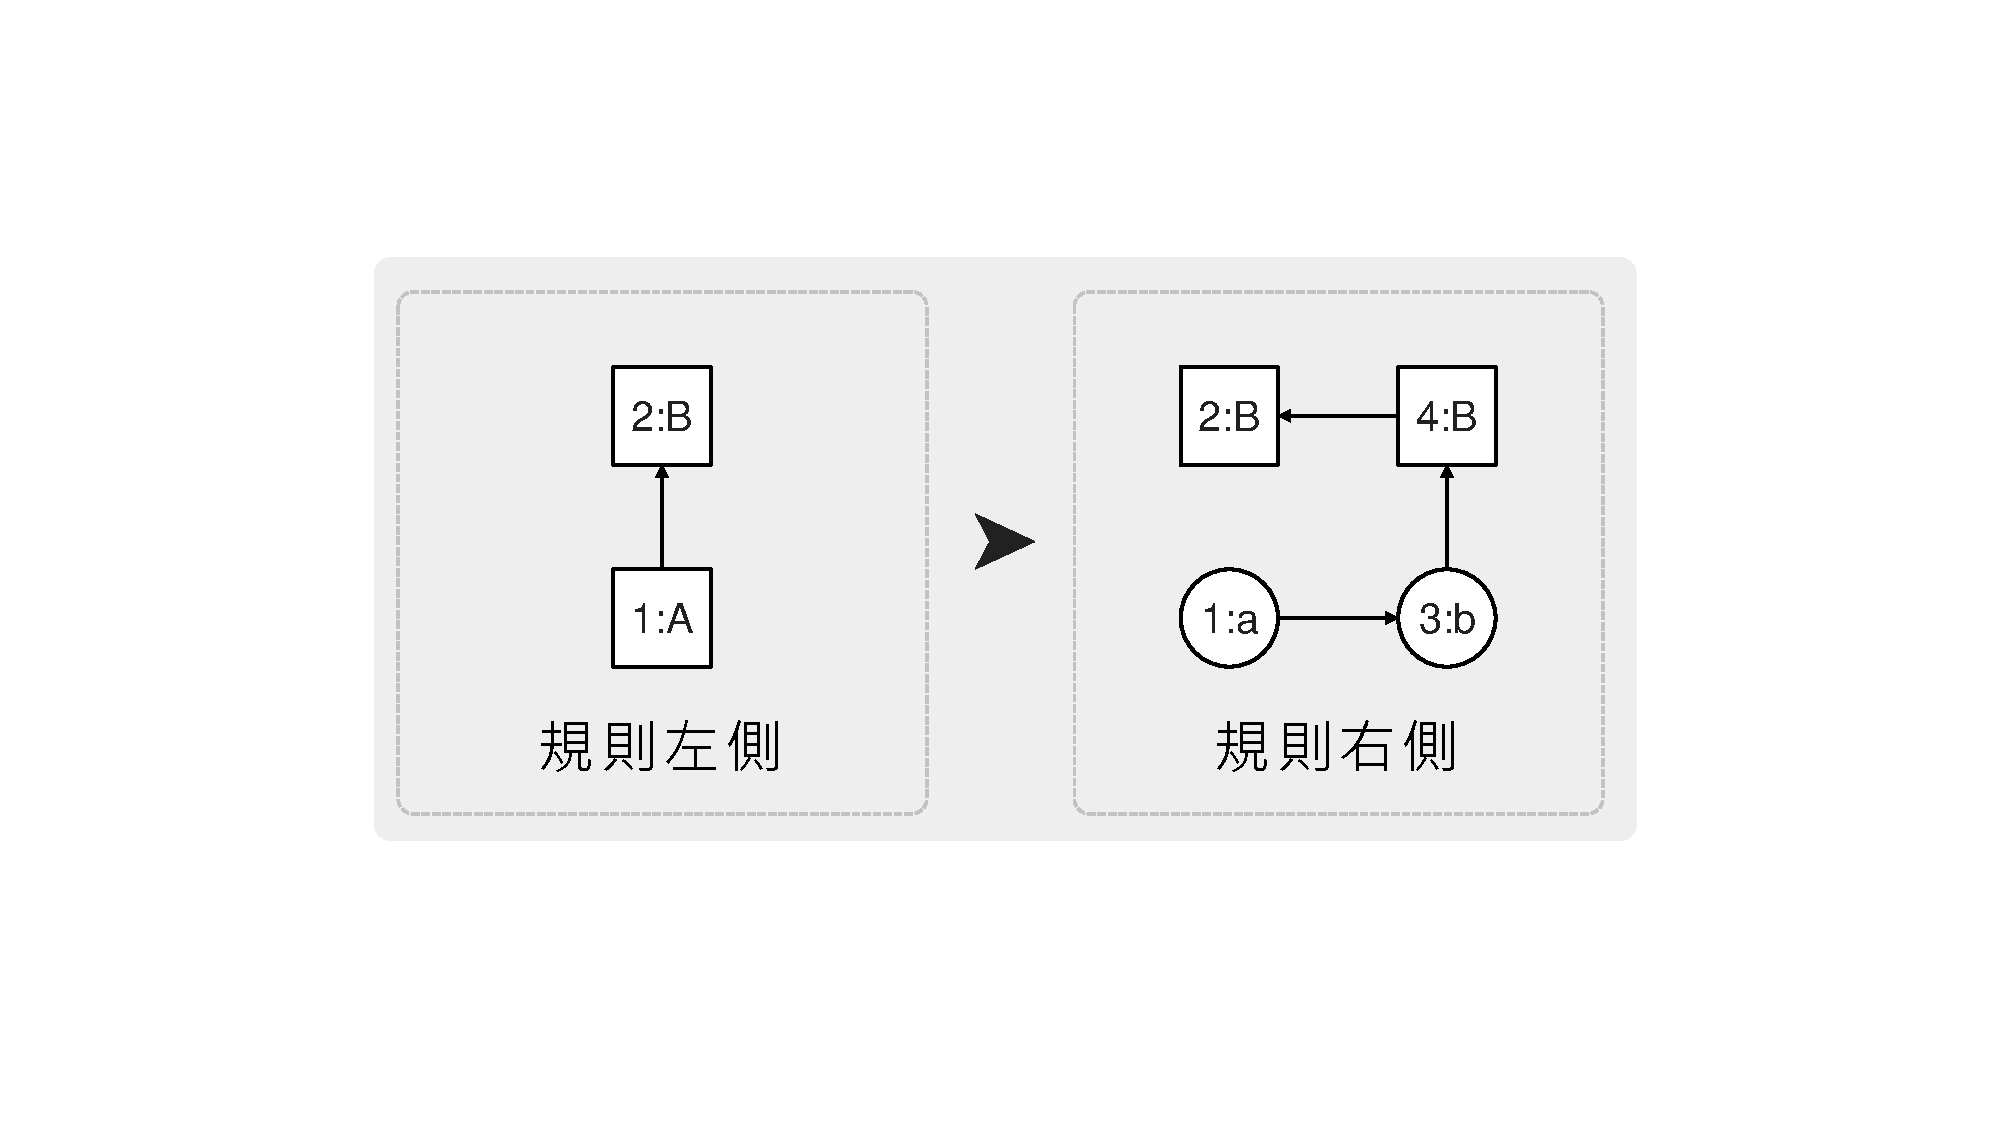
\includegraphics[width=1.0\textwidth]{figures/missiongrammars-tutorial.pdf}
    \caption{任務規則範例}
    \label{fig:missiongrammars-tutorial}
  \end{center}
\end{figure}

\subsubsection{線性任務規則}
\label{sssec:method-missiongrammars-rules-linearrules}

玩家在進行遊戲時,會有一條的主要任務流程、劇情安排。表~\ref{tbl:missiongrammars-rules-linear-example} 設計了三道任務規則,分別為主線任務、配置魔王房與探索通道。主線任務規則中,系統會從預設起始節點 (starting node) 開始進行改寫,並轉換為由終端節點起點 (entrance\missionalphabetnode{t-entrance}{5mm}) 與終點 (goal\missionalphabetnode{t-goal}{5mm}) 所構成的線性任務,其中兩節點之間由多個非終端節點的一般房 (Normal\missionalphabetnode{nt-normal}{5mm}),而非終端節點的一般房會倚賴其它規則進行後續替換。配置魔王房規則中,規則左側中定義了必須為非終端節點的一般房 (Normal\missionalphabetnode{nt-normal}{5mm}) 與終點 (goal\missionalphabetnode{t-goal}{5mm}) 相連,並改寫該一般房為魔王房 (boss\missionalphabetnode{t-boss}{5mm})。探索通道規則中,會將任務圖中的剩餘非終端節點的一般房 (Normal\missionalphabetnode{nt-normal}{5mm}) 替換為終端節點的一般房 (normal\missionalphabetnode{t-normal}{5mm})。

\begin{table}[!htb]
  \centering
  \caption{線性任務規則範例,建立主線任務}
  \label{tbl:missiongrammars-rules-linear-example}
  \bigskip
  \begin{tabular}{
    | >{\centering\arraybackslash} m{2.5cm}
    | >{\centering\arraybackslash} m{2.5cm}
      >{} m{8.5cm} | }
    \hline
    \multicolumn{1}{ |c| }{代號}
      & \multicolumn{2}{ c| }{名稱與任務規則} \\\hline
    Main Path
      & 主線任務
      & \begin{minipage}{.3\textwidth}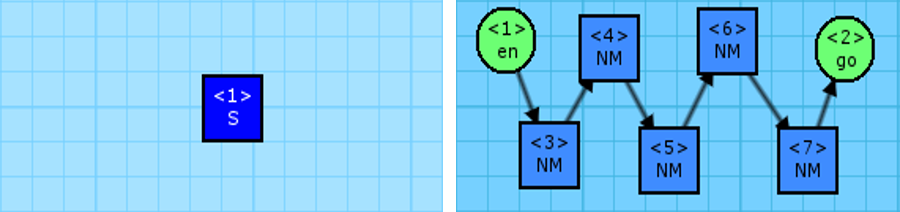
\includegraphics[width=85mm]{figures/mission-grammars-rules/main-path.png}\end{minipage}
      \\\hline
    Boss Room
      & 配置魔王房
      & \begin{minipage}{.3\textwidth}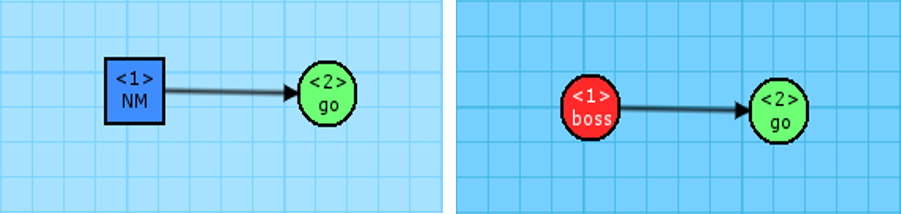
\includegraphics[width=85mm]{figures/mission-grammars-rules/boss-room.png}\end{minipage}
      \\\hline
    Exporation
      & 探索通道
      & \begin{minipage}{.3\textwidth}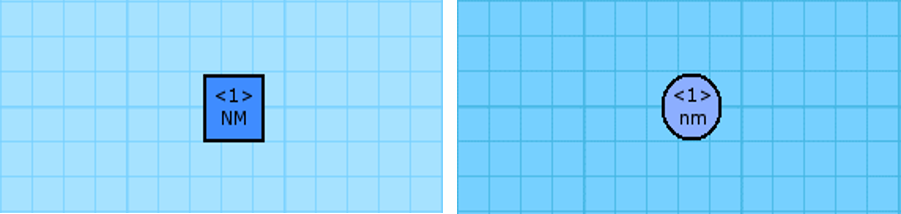
\includegraphics[width=85mm]{figures/mission-grammars-rules/exporation.png}\end{minipage}
      \\\hline
  \end{tabular}
\end{table}

結合後續第~\ref{sec:method-spacepieces} 章節 - 空間建構,並以主線任務相關規則生成任務圖後,便可將關卡輸出近似於圖~\ref{fig:missiongrammars-rules-linear-preview} 的空間。

\begin{figure}[!htb]
  \begin{center}
    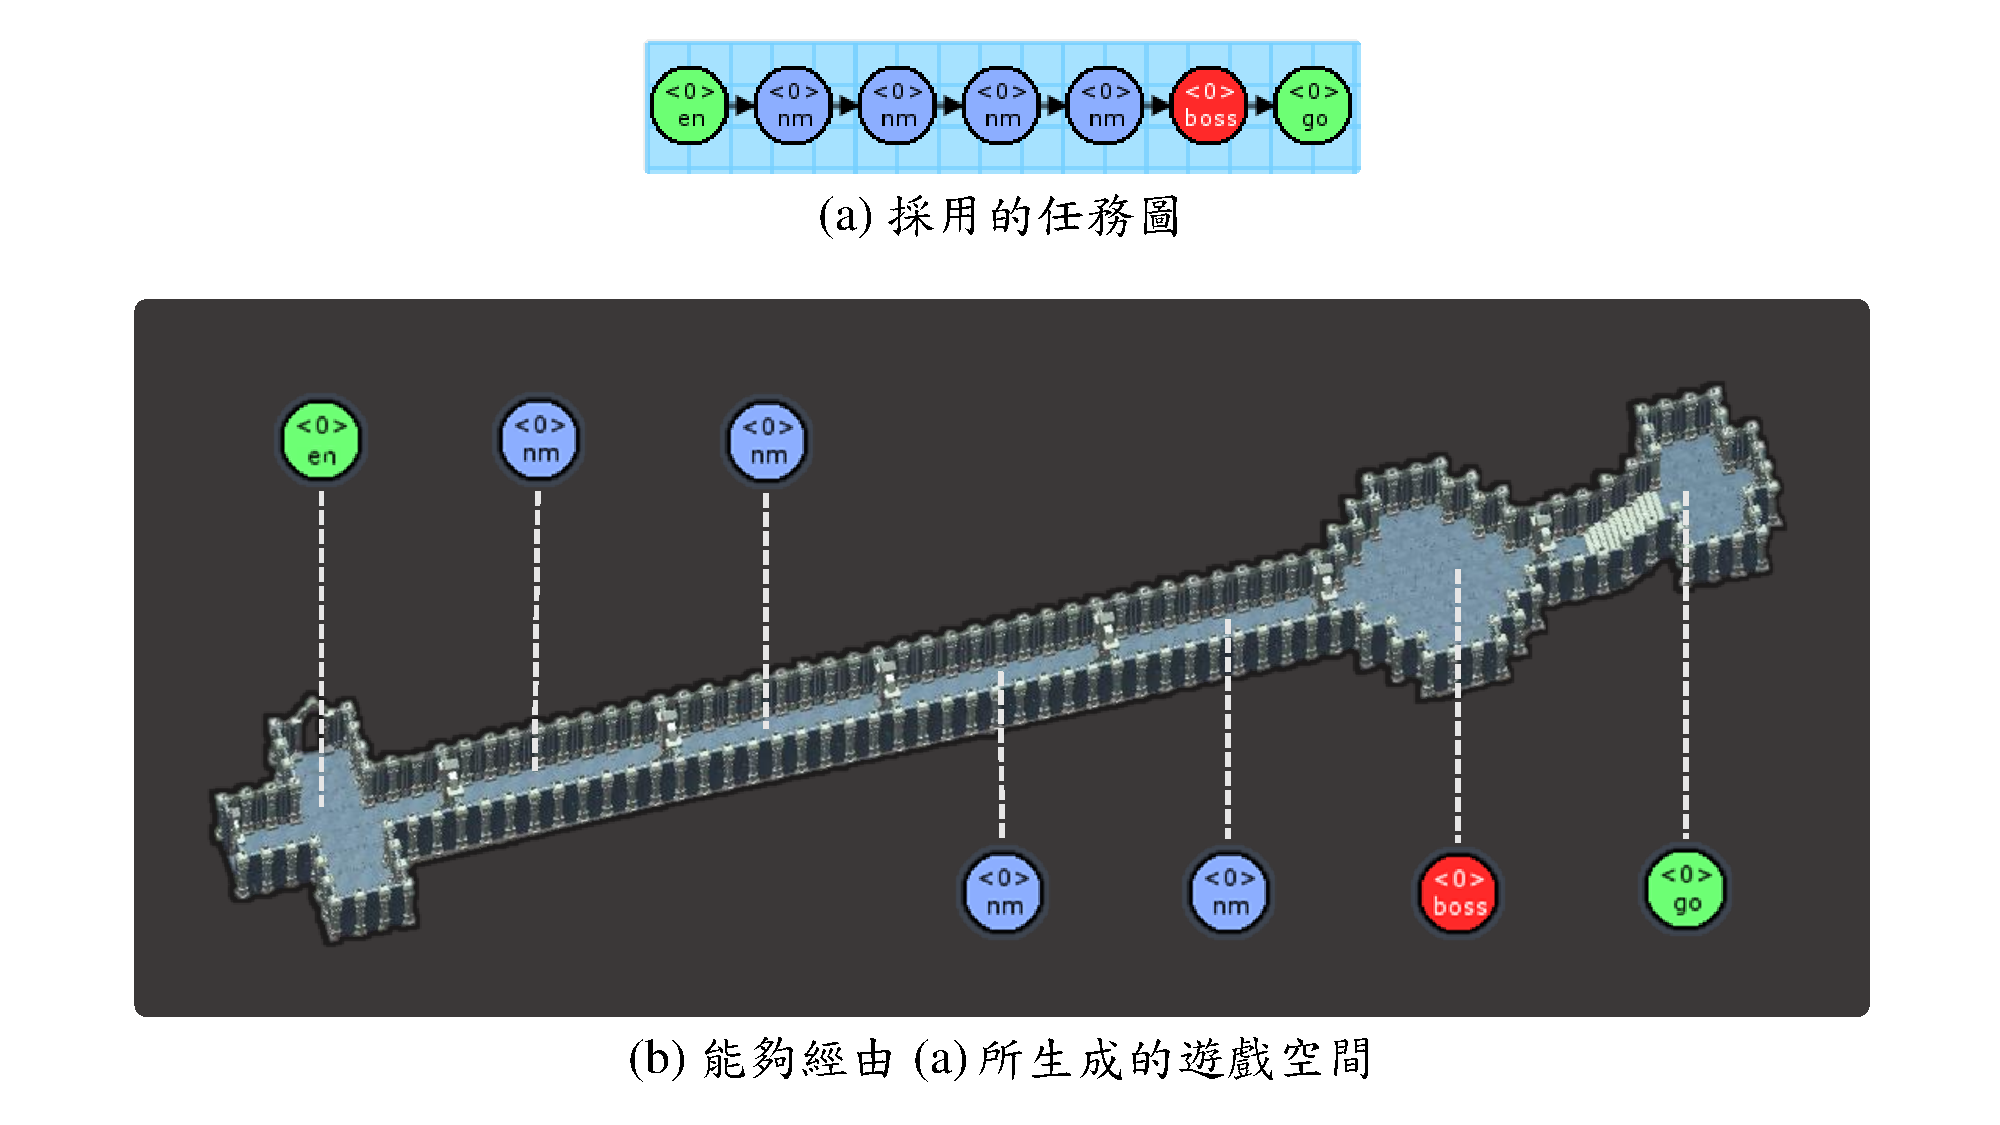
\includegraphics[width=1.0\textwidth]{figures/missiongrammars-rules-linear-preview.pdf}
    \caption{建立主線任務的預期任務圖與空間預覽}
    \label{fig:missiongrammars-rules-linear-preview}
  \end{center}
\end{figure}

\subsubsection{非線性任務規則}
\label{sssec:method-missiongrammars-rules-nonlinearrules}

為求遊戲內容的多樣性,非終端節點的一般房 (Normal\missionalphabetnode{nt-normal}{5mm}) 將有機會轉換為其它種類的遊玩特徵,表~\ref{tbl:missiongrammars-rules-nonlinear-example1} 定義了特殊房間的配置工作。配置特殊房規則中,非終端節點的一般房 (Normal\missionalphabetnode{nt-normal}{5mm}) 與任一節點相連的圖形語法(任一節點是系統保留的節點,再圖形語法中能夠表示任何的節點),會被轉換為規則右側的非線性任務圖形語法,非線性的定義是當一個節點與複數個節點連接,構成分支結構,當中的秘密房 (secret\missionalphabetnode{t-secret}{5mm}) 能夠獲取鑰匙,並有需要由炸彈才能夠突破的牆壁 (bomb\missionalphabetnode{t-bomb}{5mm}) 與其它區域阻隔,此外延伸出特殊房 (Special\missionalphabetnode{nt-special}{5mm}) 需另外定義規則使之轉換為終端節點。由於這項規則屬於較為稀少的任務類型,在套用數量上將有所限制。在商店規則與寶藏房規則中,規則左側中定義了非終端節點的特殊房 (Special\missionalphabetnode{nt-special}{5mm}) 能夠被改寫為鎖 (lock\missionalphabetnode{t-lock}{5mm}) 與商店 (shop\missionalphabetnode{t-shop}{5mm}) 或寶藏房 (treasure\missionalphabetnode{t-treasure}{5mm}) 相連的遊玩特徵。

\begin{table}[!htb]
  \centering
  \caption{非線性任務規則範例,設置特殊房}
  \label{tbl:missiongrammars-rules-nonlinear-example1}
  \bigskip
  \begin{tabular}{
    | >{\centering\arraybackslash} m{2.5cm}
    | >{\centering\arraybackslash} m{2.5cm}
      >{} m{8.5cm} | }
    \hline
    \multicolumn{1}{ |c| }{代號}
      & \multicolumn{2}{ c| }{名稱與任務規則} \\\hline
    Set Secret
      & 配置特殊房
      & \begin{minipage}{.3\textwidth}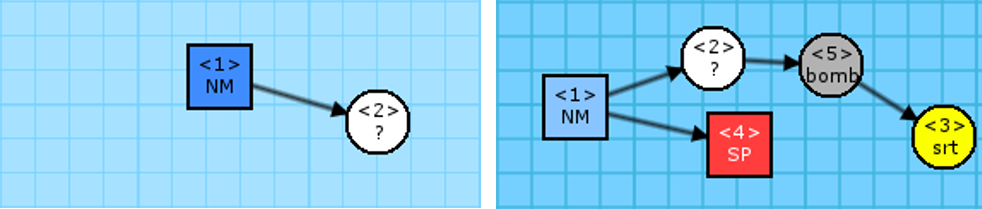
\includegraphics[width=85mm]{figures/mission-grammars-rules/set-secret.png}\end{minipage}
      \\\hline
    Shop
      & 商店
      & \begin{minipage}{.3\textwidth}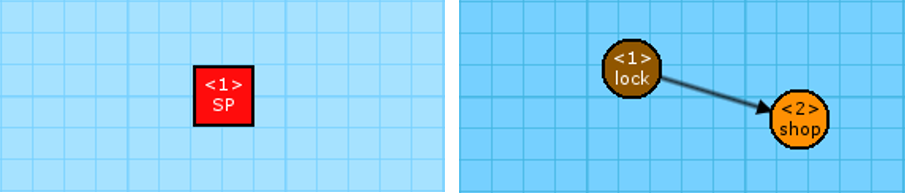
\includegraphics[width=85mm]{figures/mission-grammars-rules/shop.png}\end{minipage}
      \\\hline
    Treasure
      & 寶藏房
      & \begin{minipage}{.3\textwidth}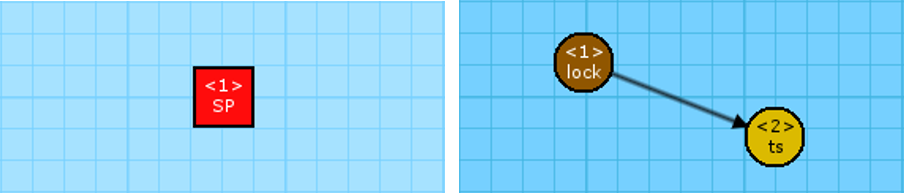
\includegraphics[width=85mm]{figures/mission-grammars-rules/treasure.png}\end{minipage}
      \\\hline
  \end{tabular}
\end{table}

表~\ref{tbl:missiongrammars-rules-nonlinear-example2},建立支線任務規則能讓指定的節點額外分支出支線任務,替換後的非終端節點一般房 (Normal\missionalphabetnode{nt-normal}{5mm}) 便能再經過其它的規則,取代成不同的遊玩特徵。

\begin{table}[!htb]
  \centering
  \caption{非線性任務規則範例,建立支線任務}
  \label{tbl:missiongrammars-rules-nonlinear-example2}
  \bigskip
  \begin{tabular}{
    | >{\centering\arraybackslash} m{2.5cm}
    | >{\centering\arraybackslash} m{2.5cm}
      >{} m{8.5cm} | }
    \hline
    \multicolumn{1}{ |c| }{代號}
      & \multicolumn{2}{ c| }{名稱與任務規則} \\\hline
    More Branch
      & 建立支線
      & \begin{minipage}{.3\textwidth}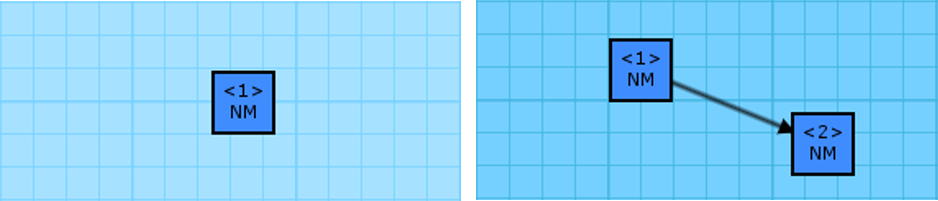
\includegraphics[width=85mm]{figures/mission-grammars-rules/more-branch.png}\end{minipage}
      \\\hline
  \end{tabular}
\end{table}

表~\ref{tbl:missiongrammars-rules-nonlinear-example3},為使玩家進行遊戲能夠提前遇見鎖 (lock\missionalphabetnode{t-lock}{5mm}),當下卻找不到鑰匙的遊玩特徵,進而思考、尋找開鎖的方式,便利用鎖向前規則將鎖的分支一同往前挪動。房間攤平規則,為避免單一房間與過多的房間連通,將部分房間進行移前推挪。

\begin{table}[!htb]
  \centering
  \caption{非線性任務規則範例,鎖的提前出現與房間攤平}
  \label{tbl:missiongrammars-rules-nonlinear-example3}
  \bigskip
  \begin{tabular}{
    | >{\centering\arraybackslash} m{2.5cm}
    | >{\centering\arraybackslash} m{2.5cm}
      >{} m{8.5cm} | }
    \hline
    \multicolumn{1}{ |c| }{代號}
      & \multicolumn{2}{ c| }{名稱與任務規則} \\\hline
    Forward Lock
      & 鎖向前
      & \begin{minipage}{.3\textwidth}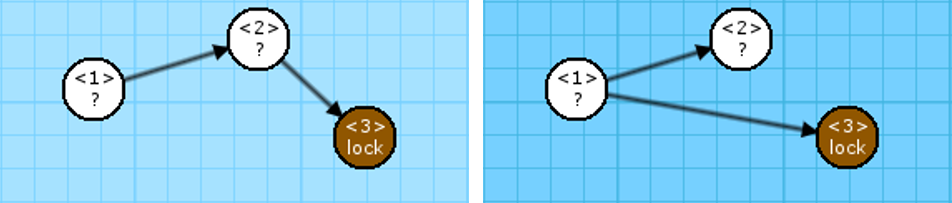
\includegraphics[width=85mm]{figures/mission-grammars-rules/forward-lock.png}\end{minipage}
      \\\hline
    Flat Rooms
      & 房間攤平
      & \begin{minipage}{.3\textwidth}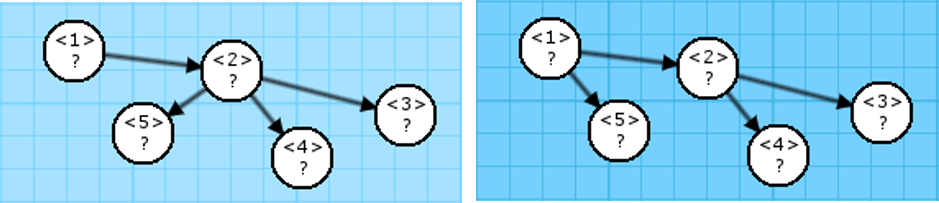
\includegraphics[width=85mm]{figures/mission-grammars-rules/flat-rooms.png}\end{minipage}
      \\\hline
  \end{tabular}
\end{table}

% \subsubsection{重複循環型任務規則}
% \label{sssec:method-missiongrammars-rules-cyclic}

% 遊戲設計師能夠依照需求定義出無窮的疊代規則,舉例來說,

\subsubsection{排除非法規則}
\label{sssec:method-missiongrammars-rules-illegals}

設計規則時,\textit{Dungeon Generator} 將排除不合法的九項設計原則,非法的設計特徵會導致改寫系統出現錯誤,見圖~\ref{fig:missiongrammars-illegal-rules}。例如:改寫系統陷入無限循環或任務圖破碎化。在表~\ref{tbl:illegal-mission-rules} 所列舉之條件於某些情況中,可能彼此會同時符合多項非法條件,系統將依照判斷順序擇一輸出。

\begin{figure}[!htb]
  \begin{center}
    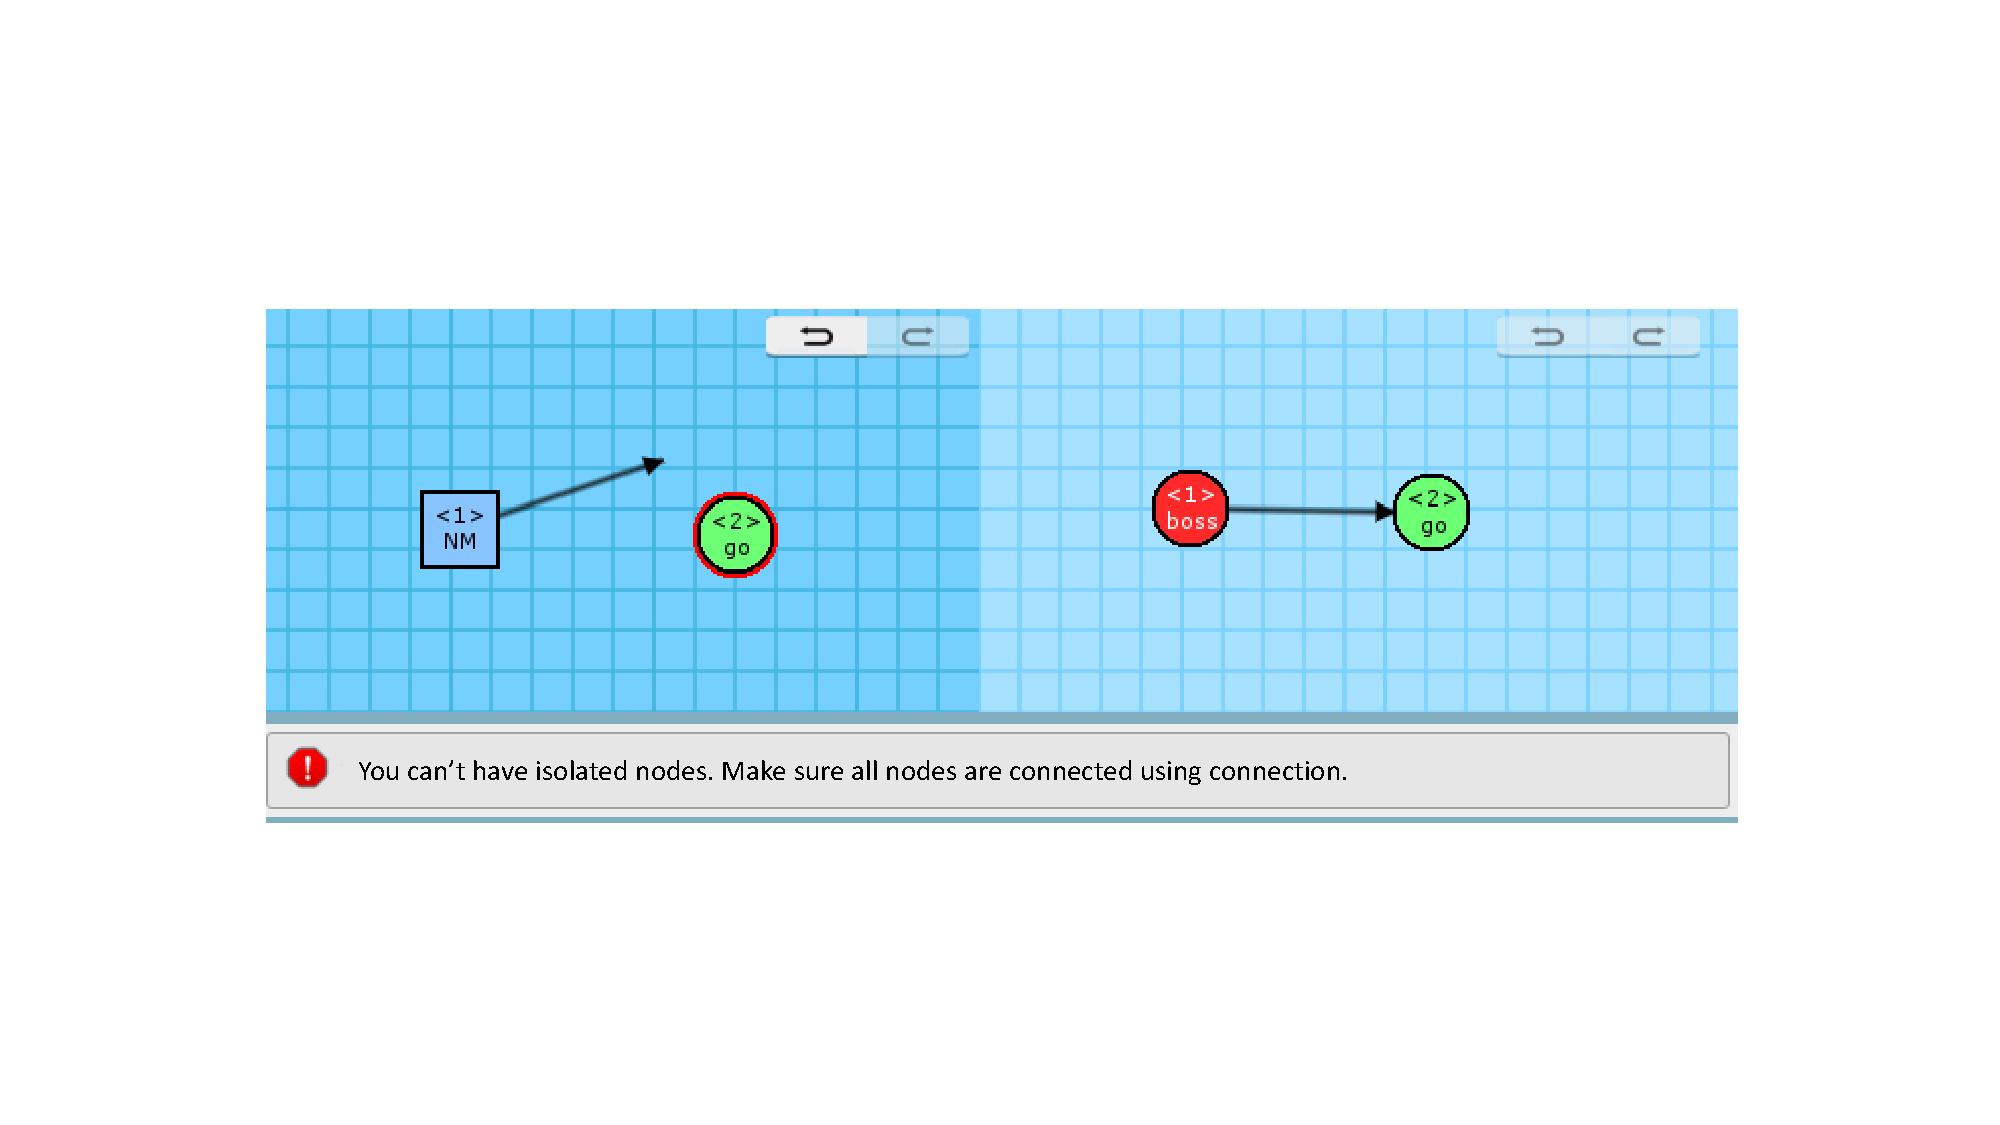
\includegraphics[width=1.0\textwidth]{figures/missiongrammars-illegal-rules.pdf}
    \caption{於 Dungeon Generator 工具中,若規則為非法狀態將不予生效}
    \label{fig:missiongrammars-illegal-rules}
  \end{center}
\end{figure}

\setlength\LTcapwidth{\linewidth}
\begin{longtable}{
    | >{\centering\arraybackslash} p{4cm}
    | >{} p{10cm} | }
  \caption{非法的任務規則定義}\label{tbl:illegal-mission-rules} \\
  \hline
  非法規則之標籤 & \multicolumn{1}{ c| }{標籤的狀況描述} \\
  \hline
  \endfirsthead
  \multicolumn{2}{c}%
  {\tablename\ \thetable\ -- \textit{接續前頁面}} \\
  \hline
  非法規則之標籤 & \multicolumn{1}{ c| }{標籤的狀況描述} \\
  \hline
  \endhead
  \multicolumn{2}{r}{\textit{接續下頁面}} \\
  \endfoot
  \endlastfoot
  LeftMoreThanRight  & 當左側的節點超過右側的節點數量時,進行改寫系統會使左側無法對應到右側的節點產生遺失的情形。若這些節點原先已有與其它非規則內節點連接,將會導致該連接資訊遺失,有機會造成任務圖破碎。 \\\hline
  EmptyLeft          & 左側為空將無法進行子圖搜索,因此左側節點必須至少一個節點。 \\\hline
  IsolatedNode       & 孤立的節點將會導致任務圖破碎。 \\\hline
  IsolatedConnection & 孤立的連接線無法正確表示其連接資訊,將無法正常進行改寫系統。 \\\hline
  ExactlyDuplicated  & 若左右規則同構將導致改寫系統陷入無限循環。 \\\hline
  MultipleRelations  & 兩兩節點間不可有超過一個的連接關係,不論是同向連接線或反向連接線皆會導致改寫系統無法正常運作。 \\\hline
  CyclicLink         & 任務圖的定義中,任務應嚴格遵守任務間之順序性,若有循環結構將會使玩家迂迴停滯。 \\\hline
  OrphanNode         & 若有圖形語法含有兩個以上的根節點,便無法正確定位出任務起點。 \\\hline
  OverflowedAnyNode  & 當規則右側使用 Any 節點時,其對應到左側索引值的節點亦必須為 Any 節點。反之,規則左側使用 Any 節點將不在此限。 \\\hline
\end{longtable}

\subsection{產生任務圖}
\label{ssec:method-missiongrammars-graph}

根據 Joris Dormans~\cite{dormans2010adventures} 提出的方法並修改至符合我方實驗需求,歸納出演算法~\ref{alg:algorithm-missiongrammars-rewritesystem} - 改寫系統(任務語法),當中會應用到演算法~\ref{alg:algorithm-matchedrule} - 搜尋匹配規則。任務語法的改寫系統運行時以深度優先搜尋法 (Depth-first search) 遍歷整個任務圖,過程中遵循圖~\ref{fig:rewrite-system-i-flow} 以下步驟順序。第一步驟,源節點會從任務規則集合中過濾出相符的規則,若有多項規則同時符合替換的條件時,系統會基於它們的關聯權重 (relative weight) 從複數個規則中依照採輪盤法 (roulette wheel selection)~\cite{lipowski2012roulette} 選擇出一項任務規則稱之為匹配規則 (matched rule),並從源節點進行與匹配規則的改寫替換,符合的條件為定義遍歷中的源節點作為新圖,而新圖存在一個子圖與匹配規則的左側之圖形語法同構,同構的參考基準為節點的符號種類,在確認子圖同構的同時,有關連的節點會標記與匹配規則一致的索引值。第二步驟,將任務圖含有索引值的節點,其相連的連接線移除。第三步驟,任務圖含有有索引值的節點取代成匹配規則右側的等價節點。第四步驟,將匹配規則右側中沒有與左側等價的節點添加至任務圖中。第五步驟,依照匹配規則右側的連接線,以相同方式放入任務圖中。最後一步驟,將任務圖中的索引值移除。

\begin{figure}[!htb]
  \begin{center}
    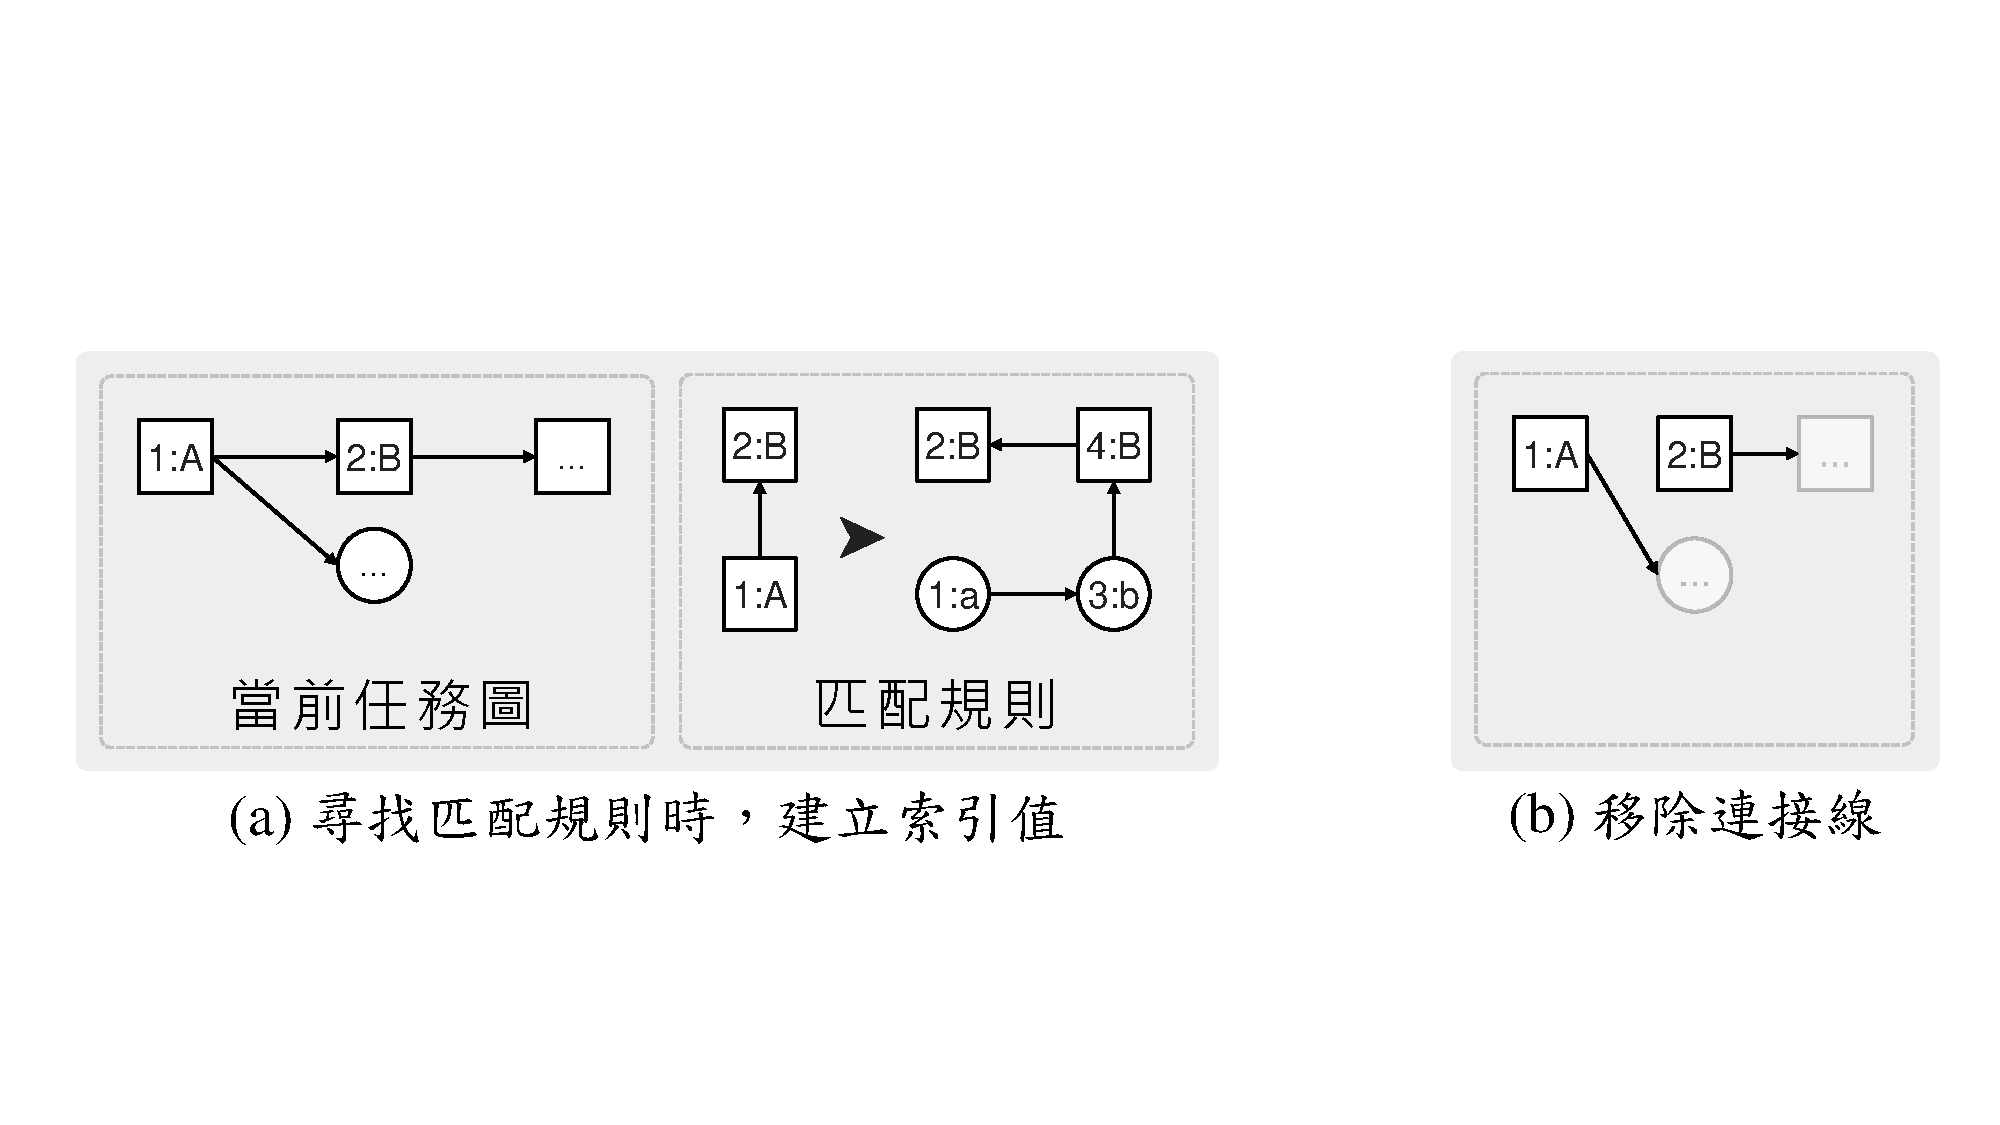
\includegraphics[width=1.0\textwidth]{figures/rewrite-system-i-flow.pdf}
    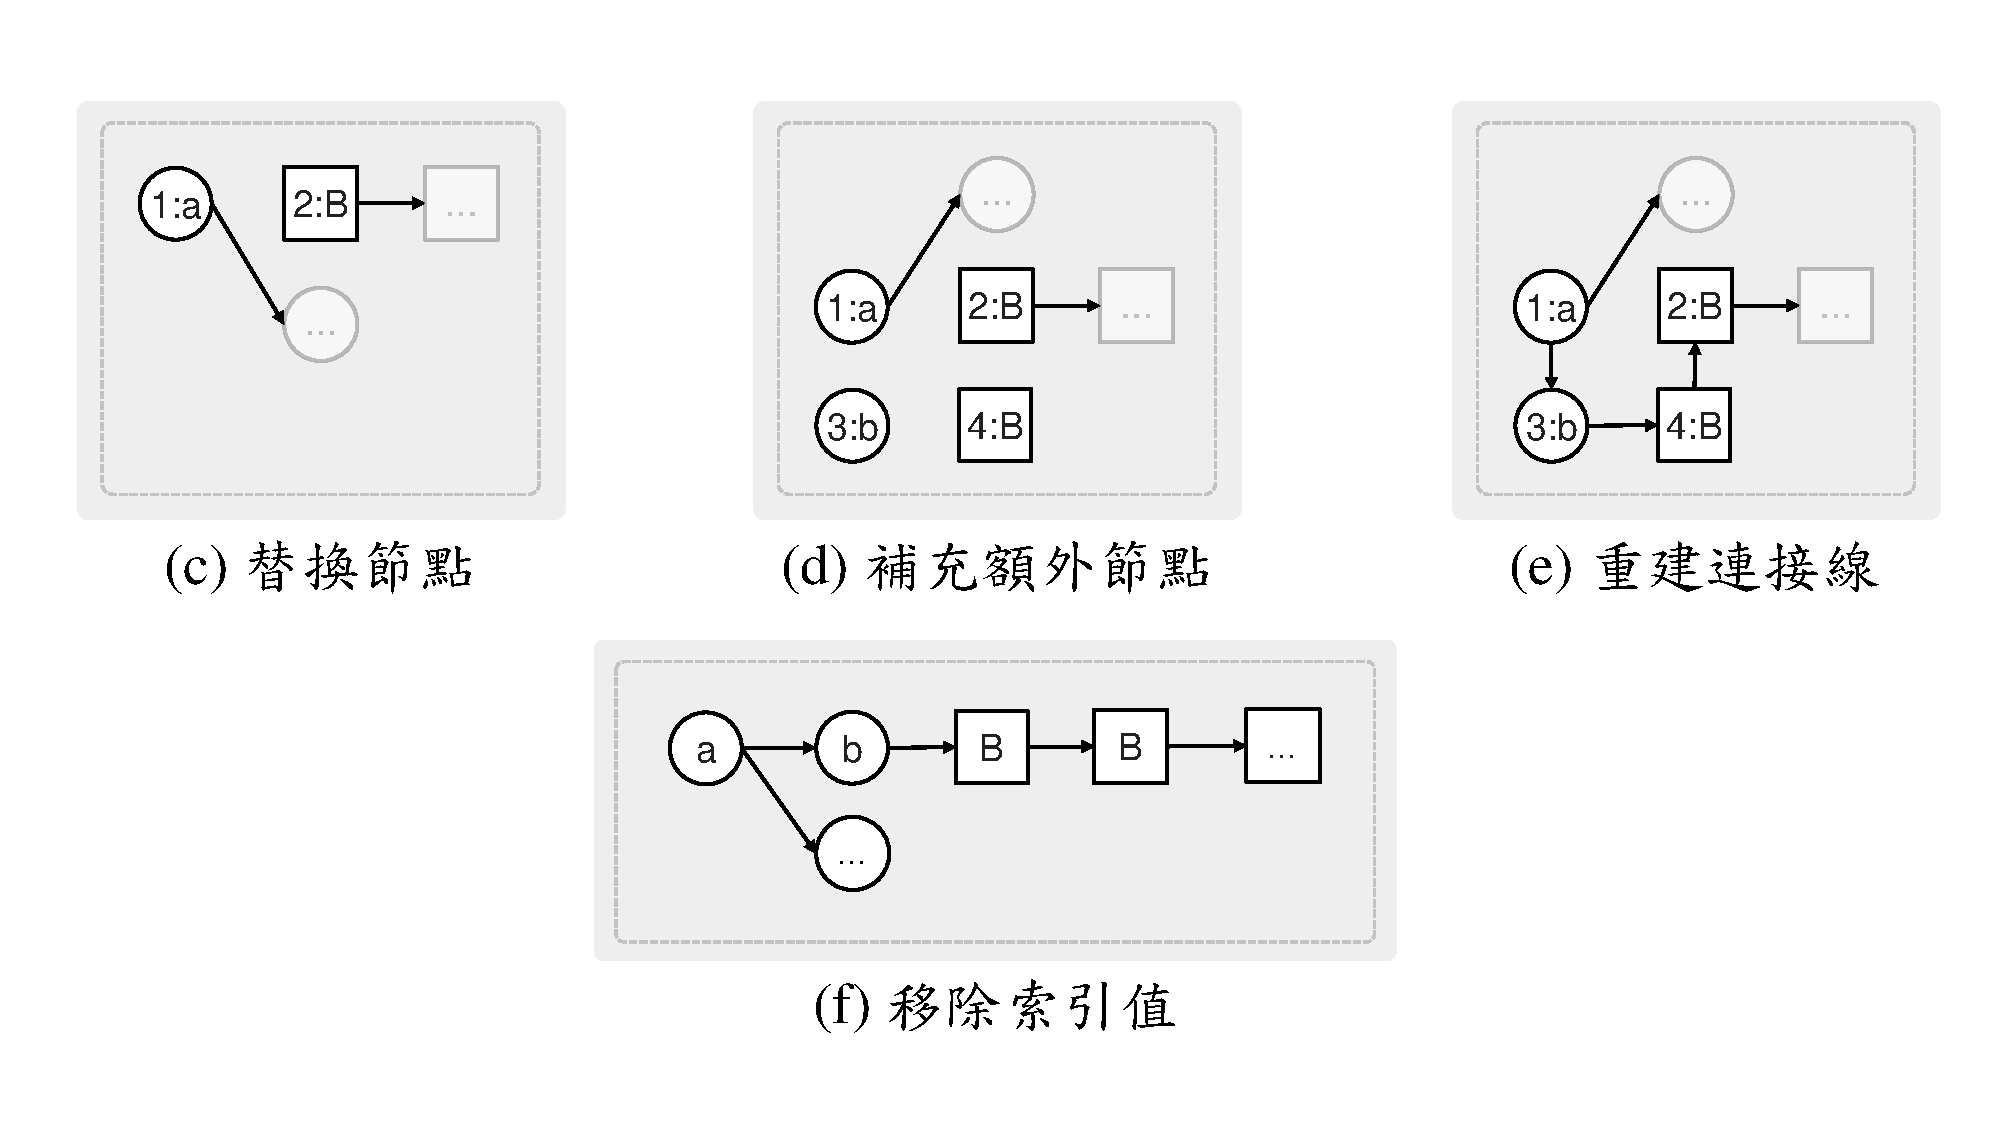
\includegraphics[width=1.0\textwidth]{figures/rewrite-system-i-flow-.pdf}
    \caption{任務語法之改寫系統流程}
    \label{fig:rewrite-system-i-flow}
  \end{center}
\end{figure}

在~\ref{ssec:method-missiongrammars-rules} 小節提及,完整的任務圖必不包含任何的非終端節點,倘若經過多次疊代改寫仍有非終端節點存在,關卡設計師必須修改任務語法其規則,使之能夠完整轉換成全終端節點的任務圖,方可進入下一階段的空間轉換。

\begin{algorithm}[!htb]
    \caption{RewriteSystem1 - 改寫系統(任務語法)}
    \label{alg:algorithm-missiongrammars-rewritesystem}
    \begin{algorithmic}[1]
        \Require
            \Statex $root$ is current $pointer$ in the mission graph.
            \Statex $rules$ is a rule set of mission grammars.
            \Statex $seed$ is the random seed.
        \Ensure
            \If {$matchedRule$ is found from $root$ and $root$ doesn't be explored}
                \State {$matchedRule$ = FindMatchs($root$)}            \Comment{演算法~\ref{alg:algorithm-matchedrule} 之方法}
                \State {移除與 $matchedRule$ 相符子圖節點間的連接線}
                \State {依照對應索引值替換成 $matchedRule$ 的規則右側}
                \State {將 $matchedRule$ 剩餘的節點填充至任務圖中}
                \State {依照 $matchedRule$ 的連接情況,移轉到任務圖中}
                \State {移除節點的索引值相關資訊}
            \EndIf
            \ForAll {$child\in children$ of $root$}:
                \State {RewriteSystem1($child$, $rules$, $seed$)}      \Comment{遞迴式,跳往 Line $1$}
            \EndFor \\
            \Return {$root$}
    \end{algorithmic}
\end{algorithm}

\begin{algorithm}[!htb]
    \caption{Part of RewriteSystem1 - 搜尋匹配規則}
    \label{alg:algorithm-matchedrule}
    \begin{algorithmic}[1]
        \Require
            \Statex $root$ is current $pointer$ in the mission graph.
        \Ensure
            \State {$matchedRules$ is an empty array of $rule$}
            \State {$graph$ = TransformToGraph($root$)}               \Comment{以該節點作為新圖之根}
            \ForAll {$rule\in$ GetAllRules()}:                        \Comment{參照任務規則表,表~\ref{tbl:missiongrammars-rules-linear-example}-~\ref{tbl:missiongrammars-rules-nonlinear-example3}}
                \If {$graph$ is isomorphic with $left$ of $rule$}     \Comment{若當前圖與該規則左側同構}
                    \State {$matchedRules$ add $rule$}                \Comment{將該規則加入候選名單}
                \EndIf
            \EndFor
            \State {$selectedRule$ = RouletteWheel($matchedRules$)}   \Comment{採輪盤法,return $rule$ or $null$}
            \State {\Return {$selectedRule$}}
    \end{algorithmic}
\end{algorithm}

圖~\ref{fig:mission-graph-generating-progress} 根據任務規則表(表~\ref{tbl:missiongrammars-rules-linear-example}-~\ref{tbl:missiongrammars-rules-nonlinear-example3})生成任務圖,並使用亂數種子 $894730$ 作舉例,每次的疊代生成依照演算法~\ref{alg:algorithm-missiongrammars-rewritesystem} 將當前任務圖的所有節點遍歷。根據前述章節定義,當圖~\ref{fig:mission-graph-generating-progress} d 時已不存在非終端節點,任務圖已趨穩定,但因為鎖向前規則與房間攤平規則,其規則左側皆為終端節點的情形下,儘管任務圖已趨穩定,只要任務圖中仍有同構子圖存在,改寫系統便能持續運行下去。在 \textit{Dungeon Generator} 中,亂數種子會同時決定一隨機次數,讓已趨穩定的任務圖仍能夠在有限次數下持續進行疊代,直至無任何規則可以被採用,見圖~\ref{fig:mission-graph-generating-progress} g。在圖~\ref{fig:final-mission-graph} 中展示了根據不同亂數種子,能夠得到豐富結果的任務圖。

\begin{figure}[!htb]
  \begin{center}
    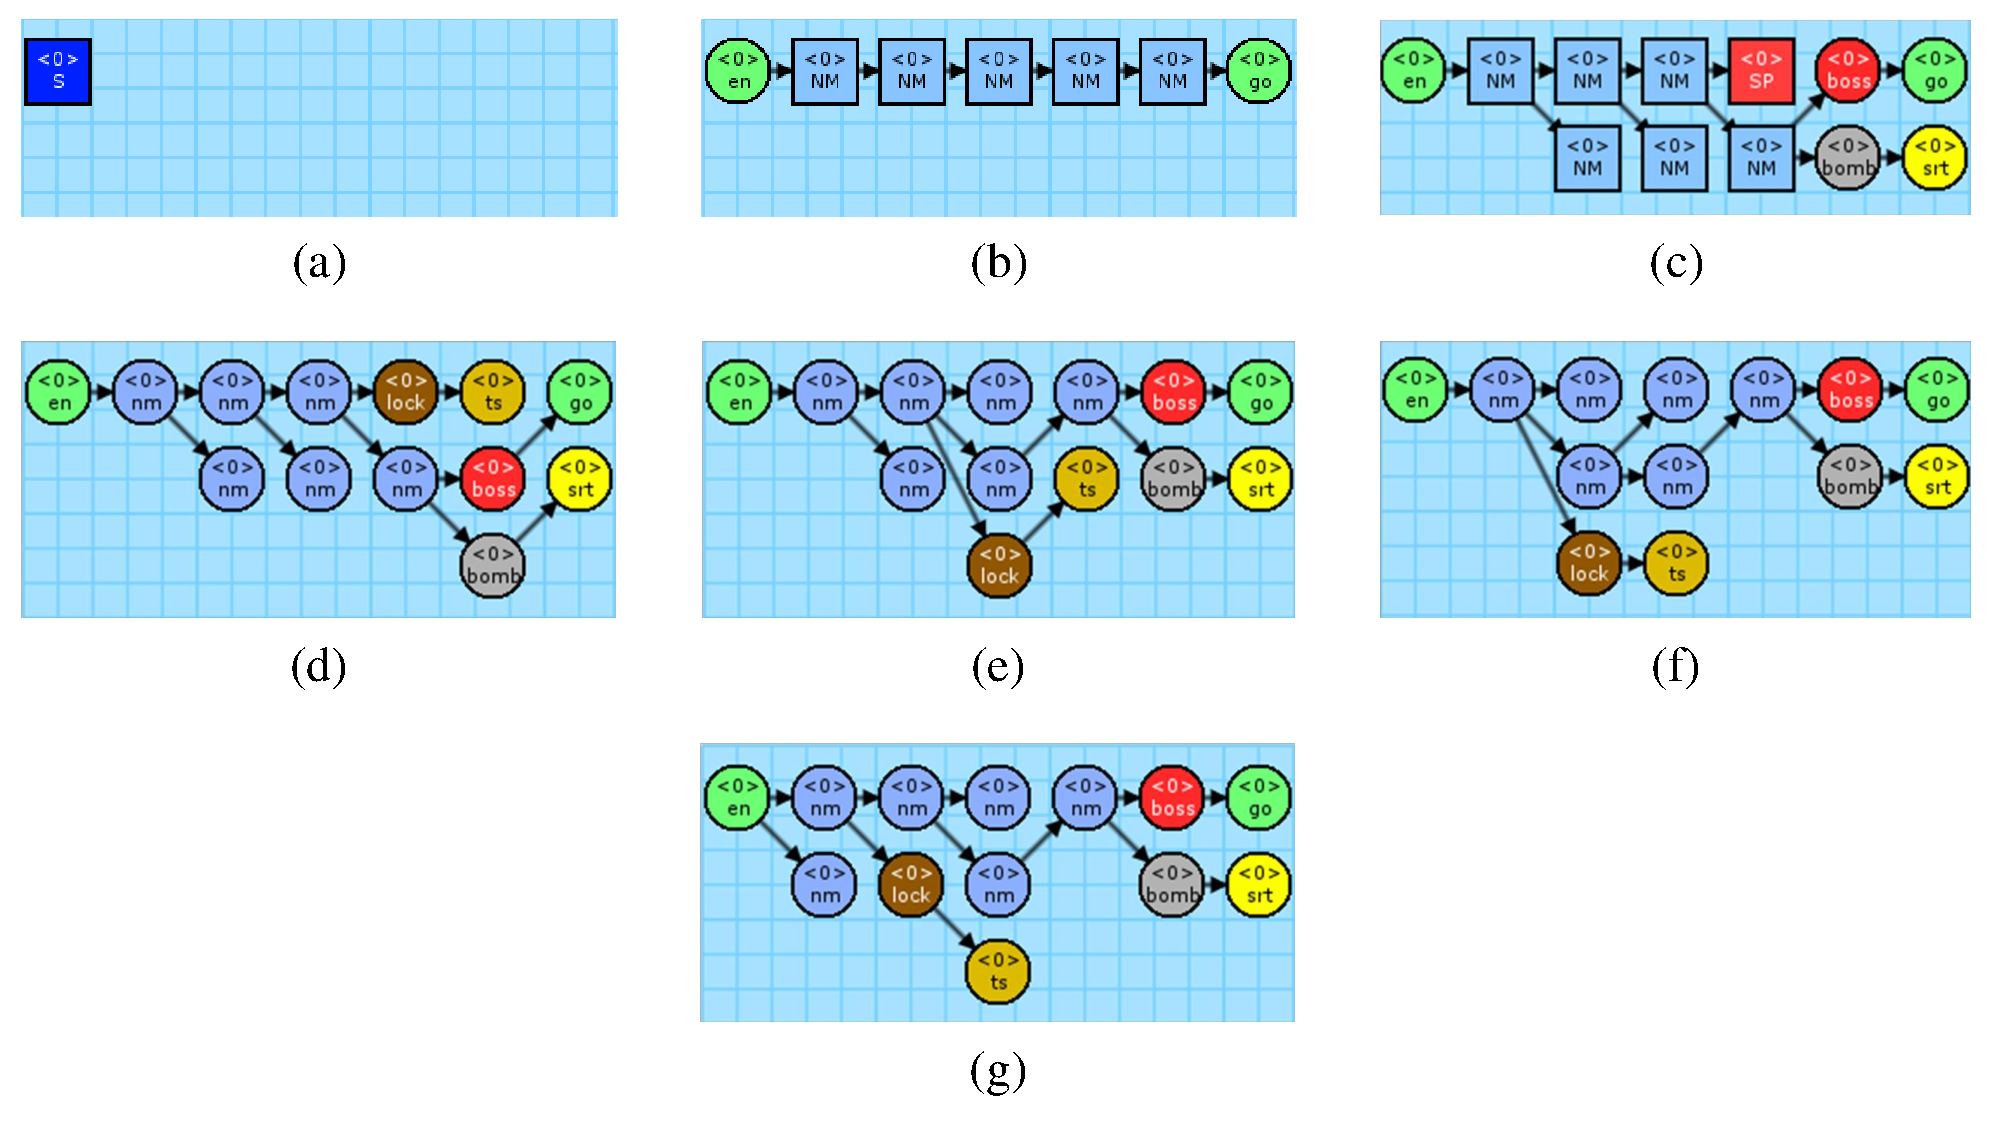
\includegraphics[width=1.0\textwidth]{figures/mission-graph-generating-progress.pdf}
    \caption{任務圖的生成過程}
    \label{fig:mission-graph-generating-progress}
  \end{center}
\end{figure}

\begin{figure}[!htb]
  \begin{center}
    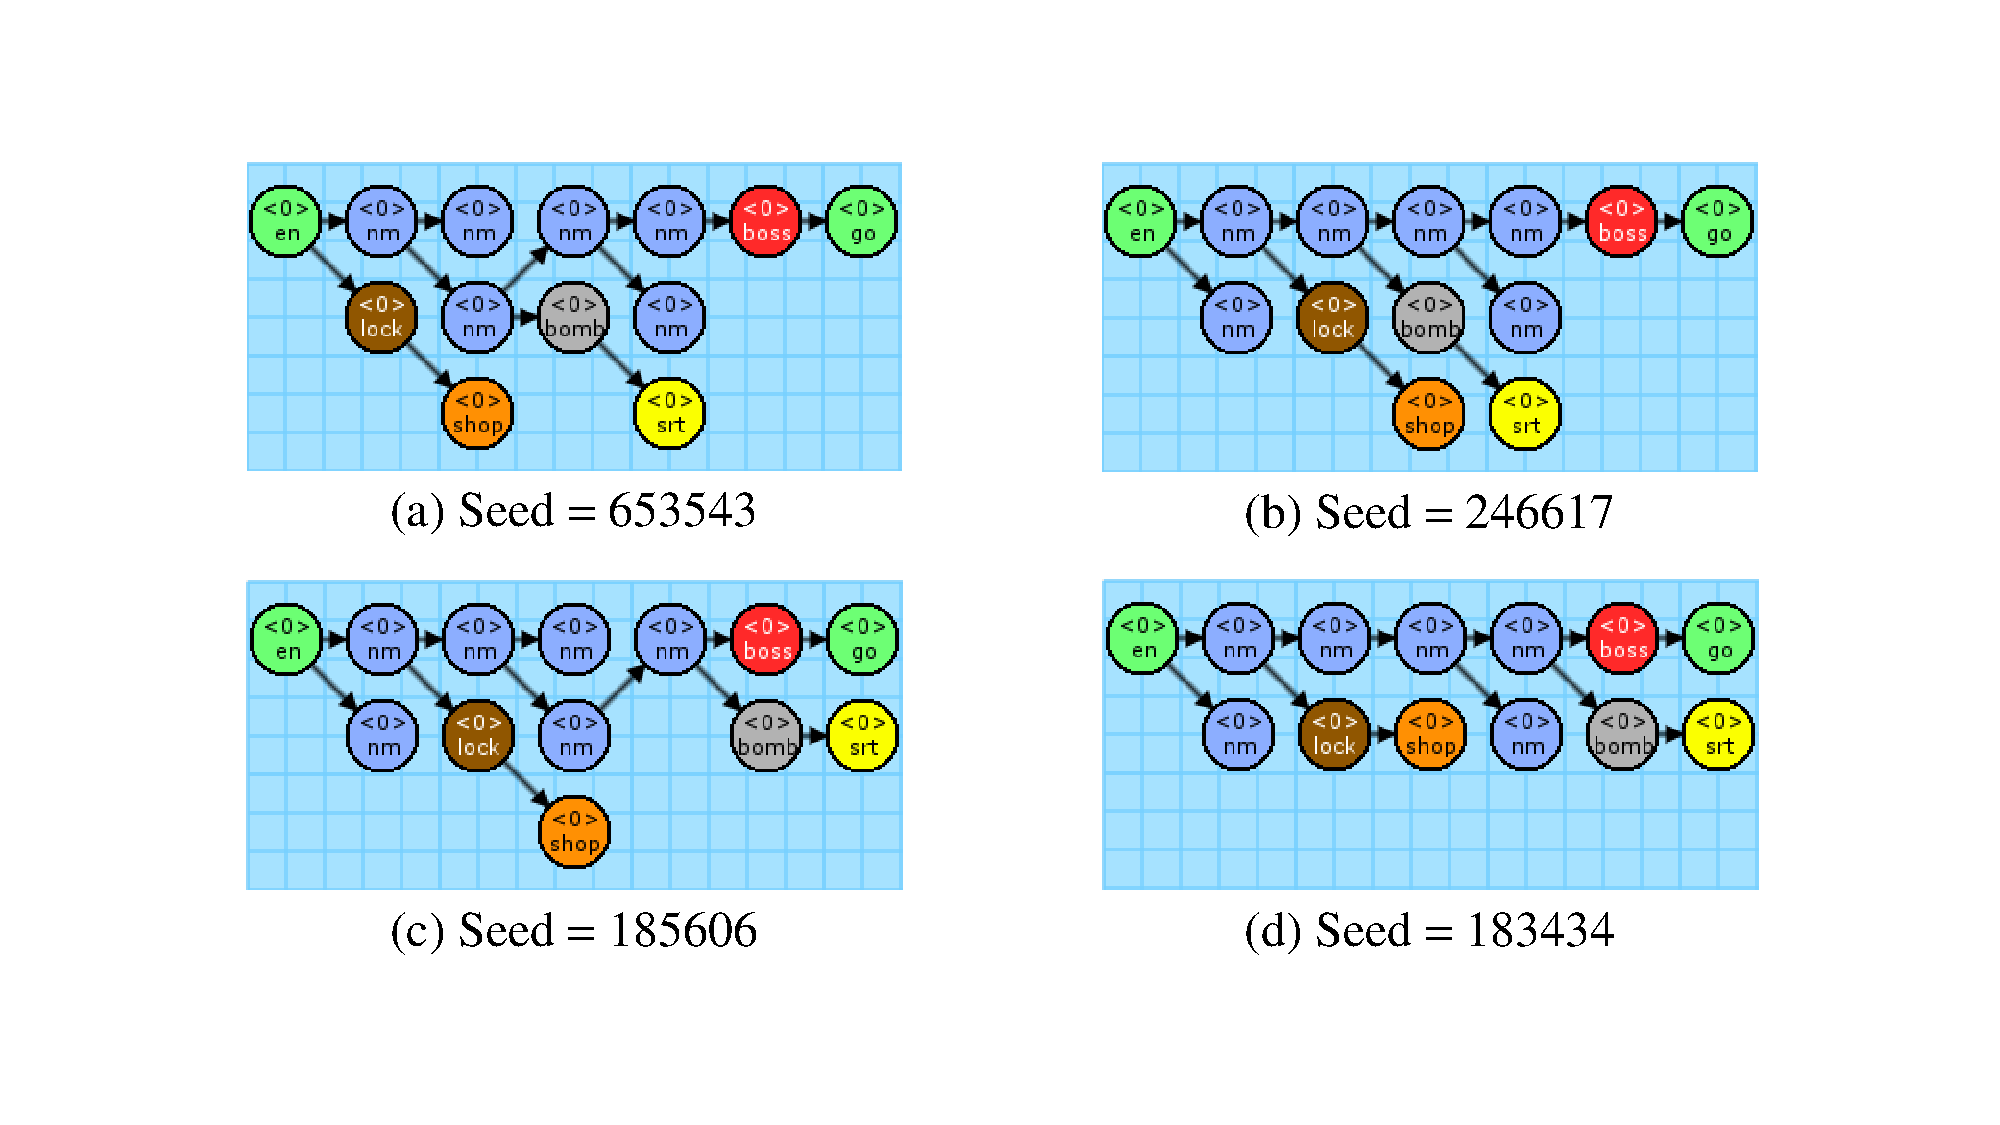
\includegraphics[width=1.0\textwidth]{figures/final-mission-graph.pdf}
    \caption{根據不同亂數種子所輸出的任務圖}
    \label{fig:final-mission-graph}
  \end{center}
\end{figure}

% Clean the page after this section.
\clearpage

\section{空間建構}
\label{sec:method-spacepieces}

Joris Dormans 於文獻中提到為二維空間的範例~\cite{dormans2010adventures}~\cite{dormans2012engineering},我們的實驗環境以三維空間為主。在空間語法中將直接構築遊戲的基礎房型,但不設置怪物、寶箱或陷阱足以直接影響遊戲性的遊戲物件,如圖~\ref{fig:gameobject-list}。此外,我們希望空間中的遊戲物件能夠有意義的自動化配置,即在設計空間語法的流程中,忽略絕大部分的遊戲物件配置,直到~\ref{sec:method-segments} 節提出之方法達成。

\begin{figure}[!htb]
  \begin{center}
    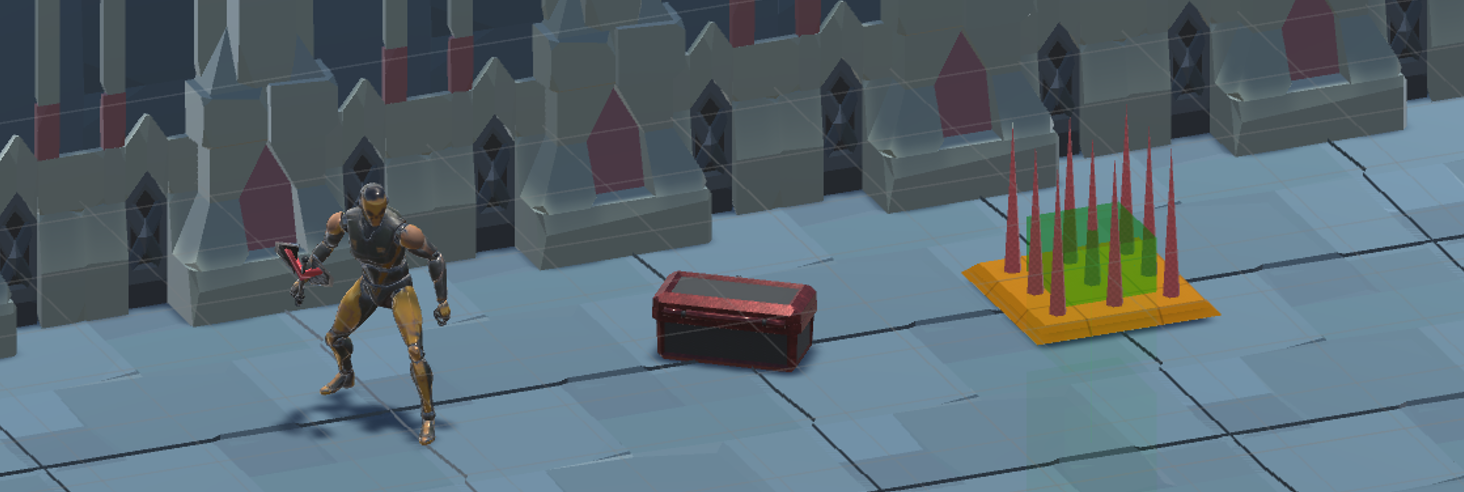
\includegraphics[width=1.0\textwidth]{figures/gameobject-list.png}
    \caption{影響遊戲性的遊戲物件,由左至右分別為敵方、寶箱與陷阱} 
    \label{fig:gameobject-list}
  \end{center}
\end{figure}

\subsection{基礎結構}
\label{ssec:method-spacepieces-basic}

我們對於空間語法做了修改以利實驗環境建置。在一個關卡 (level) 中包含數個房間容器 (volumes),每一房間容器由不定數量的房間塊 (chucks) 組成,且房間塊固定以 $9\times 9\times 9$ 個長方體體素 (voxels) 所構成,每一體素的大小為 $3\times 2\times 3$。

此外,每一個體素被分為九種方向,分別為正四方、斜四方與中心點。圖~\ref{fig:decorations-with-directions} a-c 可見,不同的裝飾物會依照其特性決定能夠放置的方位,如地面則放置於中心點;牆壁、階梯或門放置於正四方;牆壁柱放置於斜四方。在一個體素中,多個裝飾物是能夠同時並存的,例如在其放置地面、一道牆壁、兩道牆壁柱。在本次實驗環境中,我們將會使用圖~\ref{fig:decorations-with-directions} d-g 中,「地面、階梯、牆壁、牆壁柱、門」共五種裝飾物進行房間容器的體素建置工作。

\begin{figure}[!htb]
  \begin{center}
    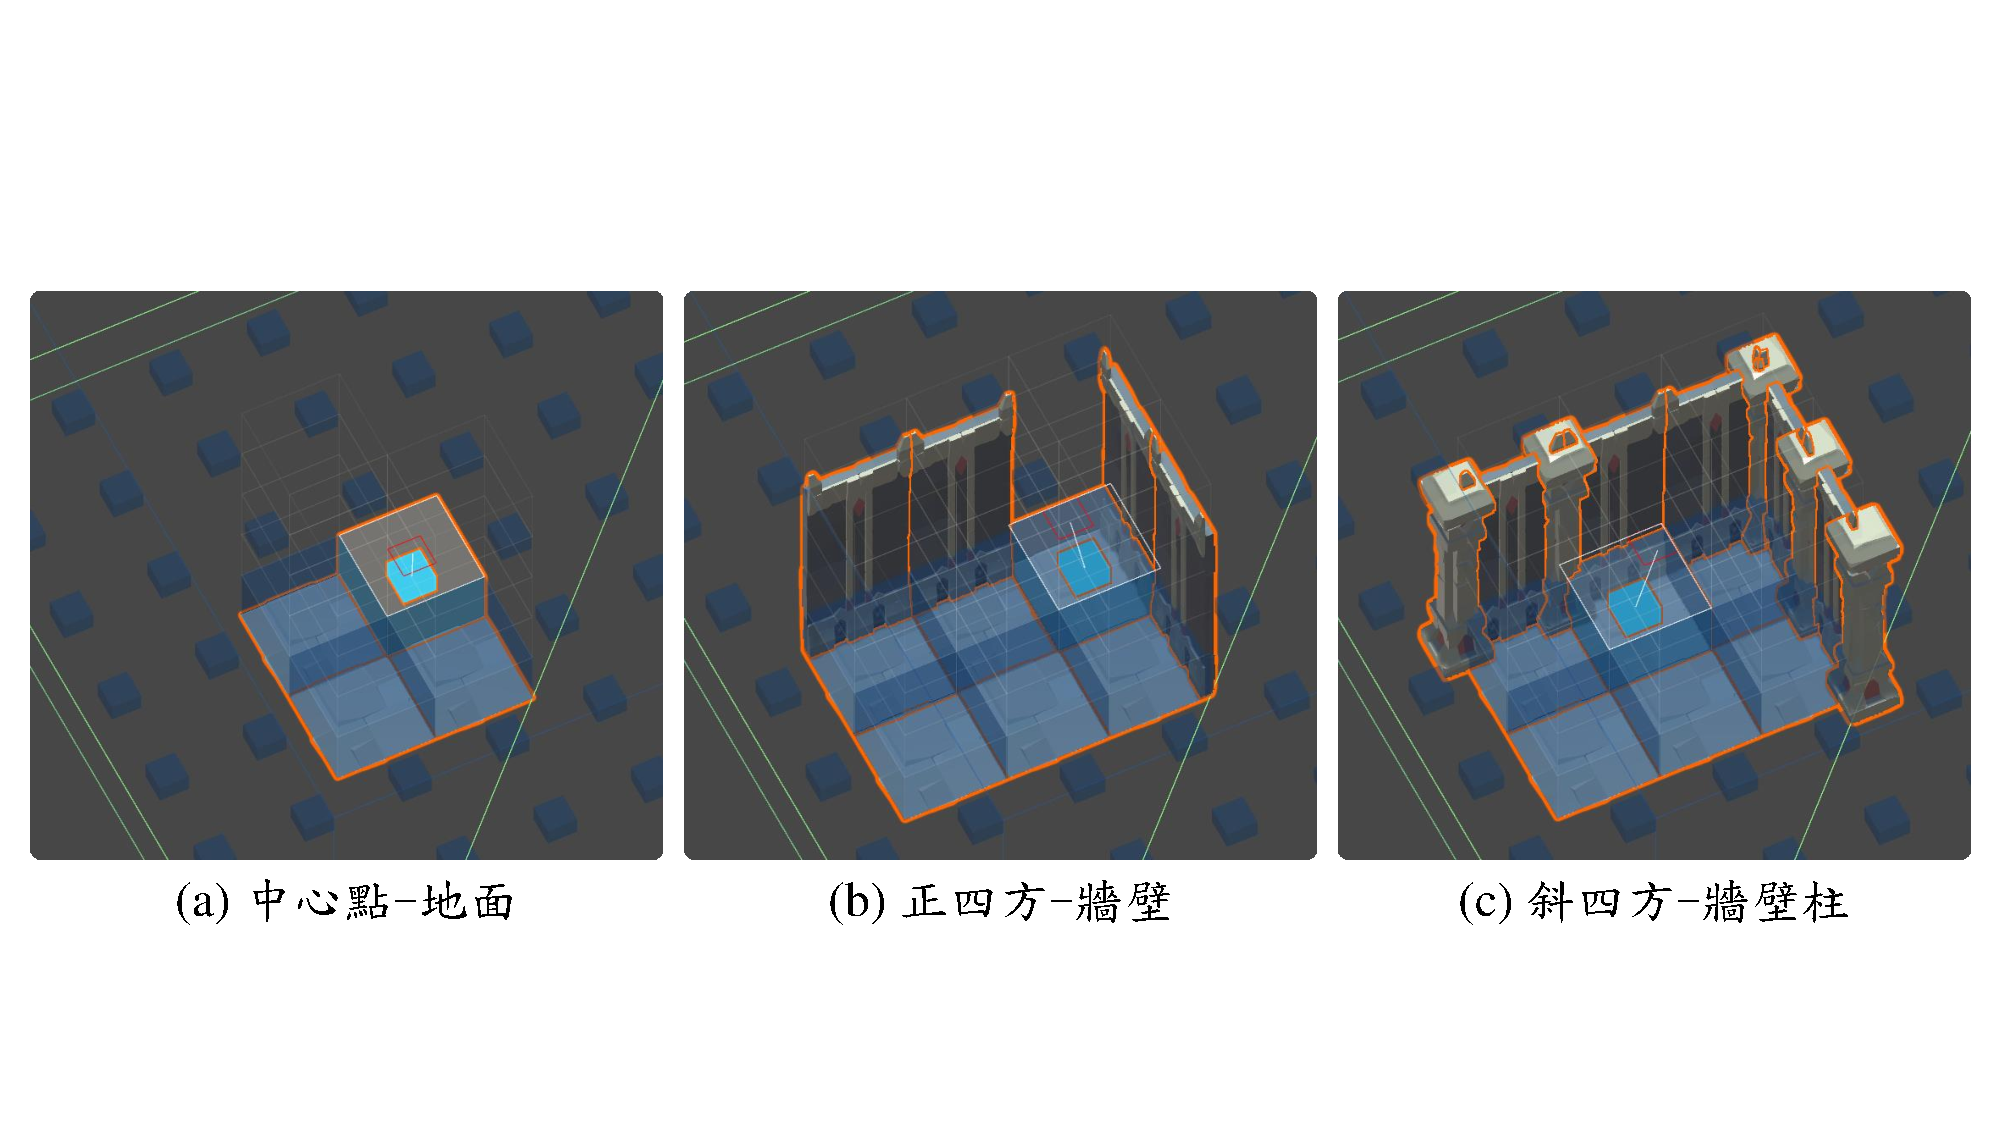
\includegraphics[width=1.0\textwidth]{figures/decorations-with-directions.pdf}
    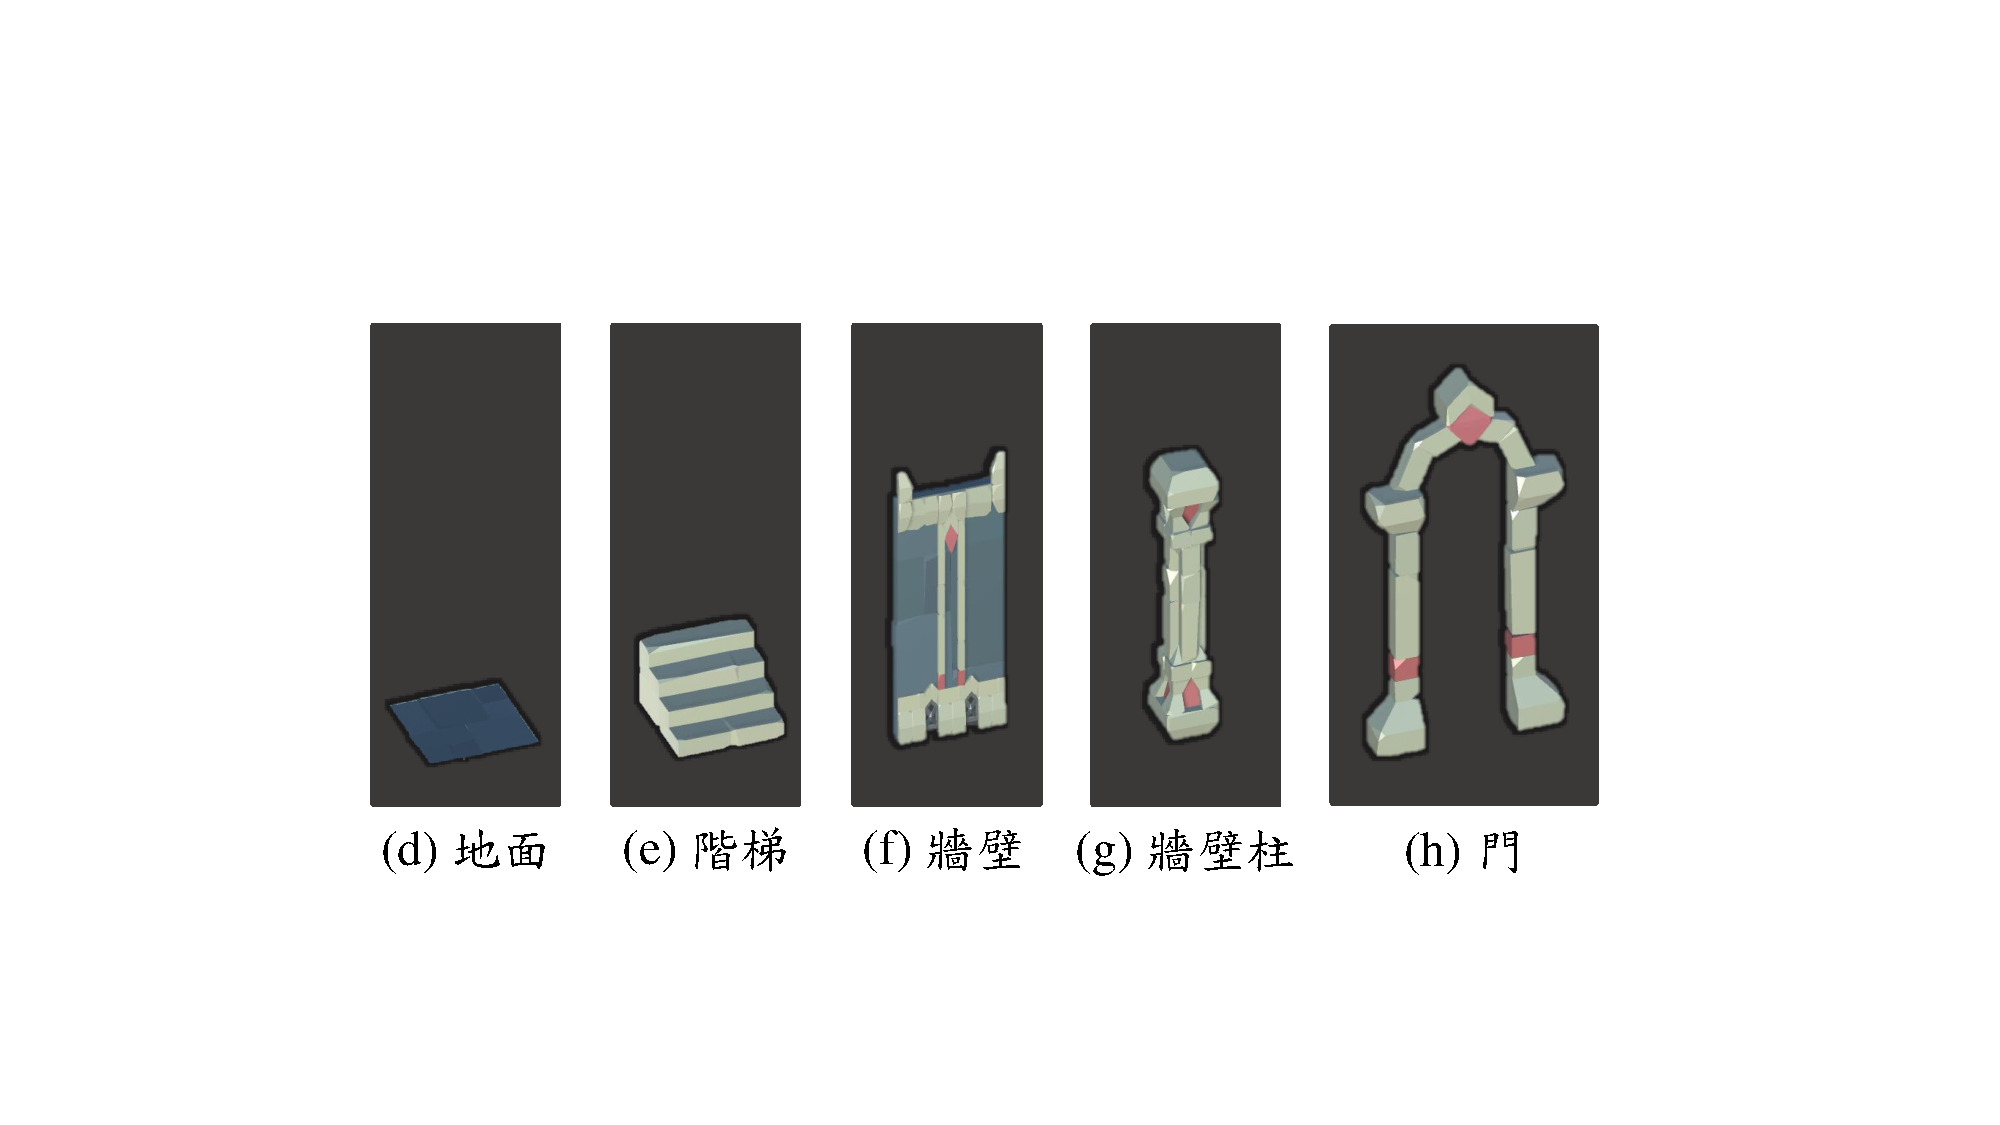
\includegraphics[width=1.0\textwidth]{figures/decorations-with-directions-.pdf}
    \caption{房間容器的體素建置方式,與五種裝飾物}
    \label{fig:decorations-with-directions}
  \end{center}
\end{figure}

\subsection{端點識別物}
\label{ssec:method-spacepieces-connections}

逐一設計出各式各樣的房間容器後,必須正確地將個空間相互連接。參考 Joris Dormans 的空間語法~\cite{dormans2012engineering},我們為體素型的房間容器添加端點識別物 (connections),而端點可再細分為入口 (entrance) 與出口 (exit),依照遊戲設計師需求,能夠自行擴充出口的類型,可為複數個出口識別物。在一房間容器中,最多僅能擁有一個入口識別物,而出口識別物的數量不在此限,且二者之數量總和必大於零。倘若空間當中沒有一個以上入口識別物,便會從現有的出口識別物中隨機挑選一與入口識別物相同功能執行之。圖~\ref{fig:connections-in-volume} 中描述了端點識別物的使用情境,入口的箭頭朝向空間內部,而出口的箭頭會朝向空間外部。

\begin{figure}[!htb]
  \begin{center}
    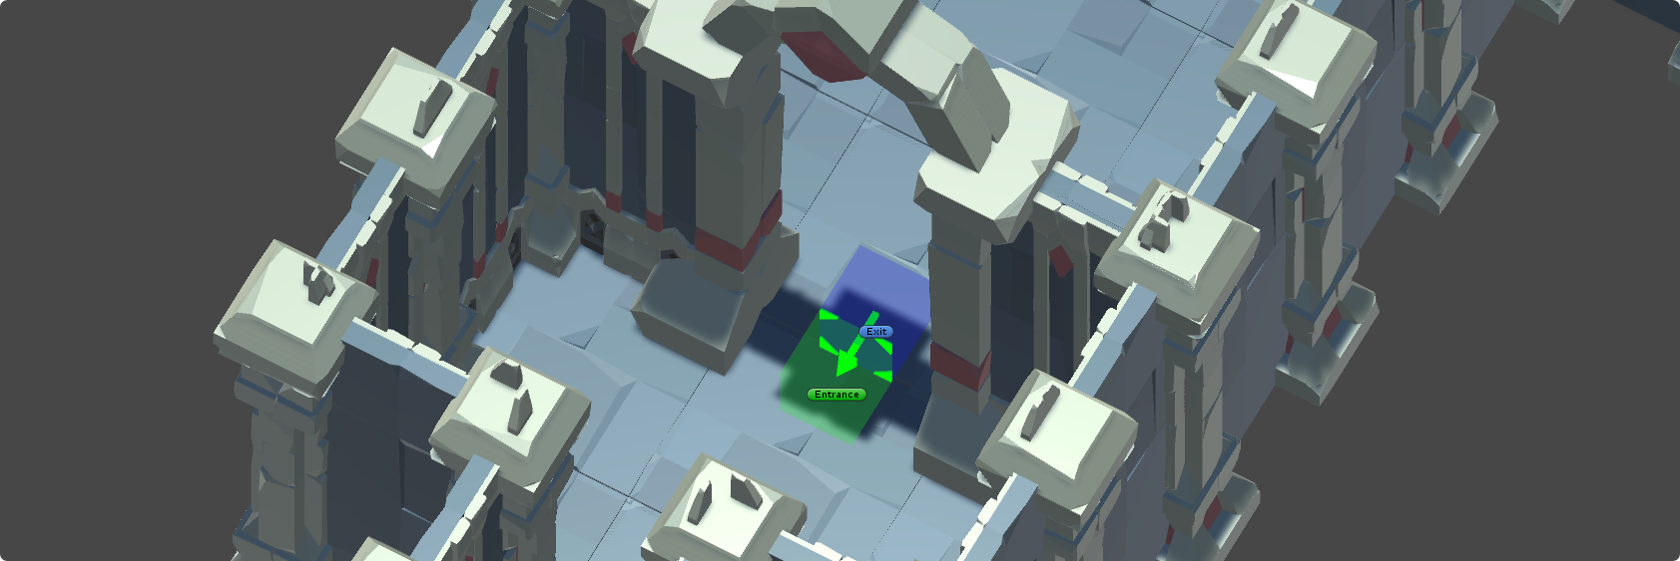
\includegraphics[width=1.0\textwidth]{figures/connections-in-volume.png}
    \caption{端點識別物的實際使用與串接情形} 
    \label{fig:connections-in-volume}
  \end{center}
\end{figure}

\subsection{房間容器類型}
\label{ssec:method-spacepieces-types}

延續第~\ref{sec:method-missiongrammars} 節任務語法所定義的任務終端節點,依照節點性質設計房型,區分出數項不同房型的空間規劃。

\subsubsection{起點、終點、魔王房}
\label{sssec:method-spacepieces-types-mainpath-i}

圖~\ref{fig:roomtype-mainpath-i}為 a 起點擁有一個入口與三個出口,為玩家重生的起始房間;圖~\ref{fig:roomtype-mainpath-i} b 為終點擁有一個入口,為遊戲關卡結束的房間;圖~\ref{fig:roomtype-mainpath-i}為 c 為魔王房擁有一個入口與一個出口,玩家會在此房間遭遇強大敵人。

\begin{figure}[!htb]
  \begin{center}
    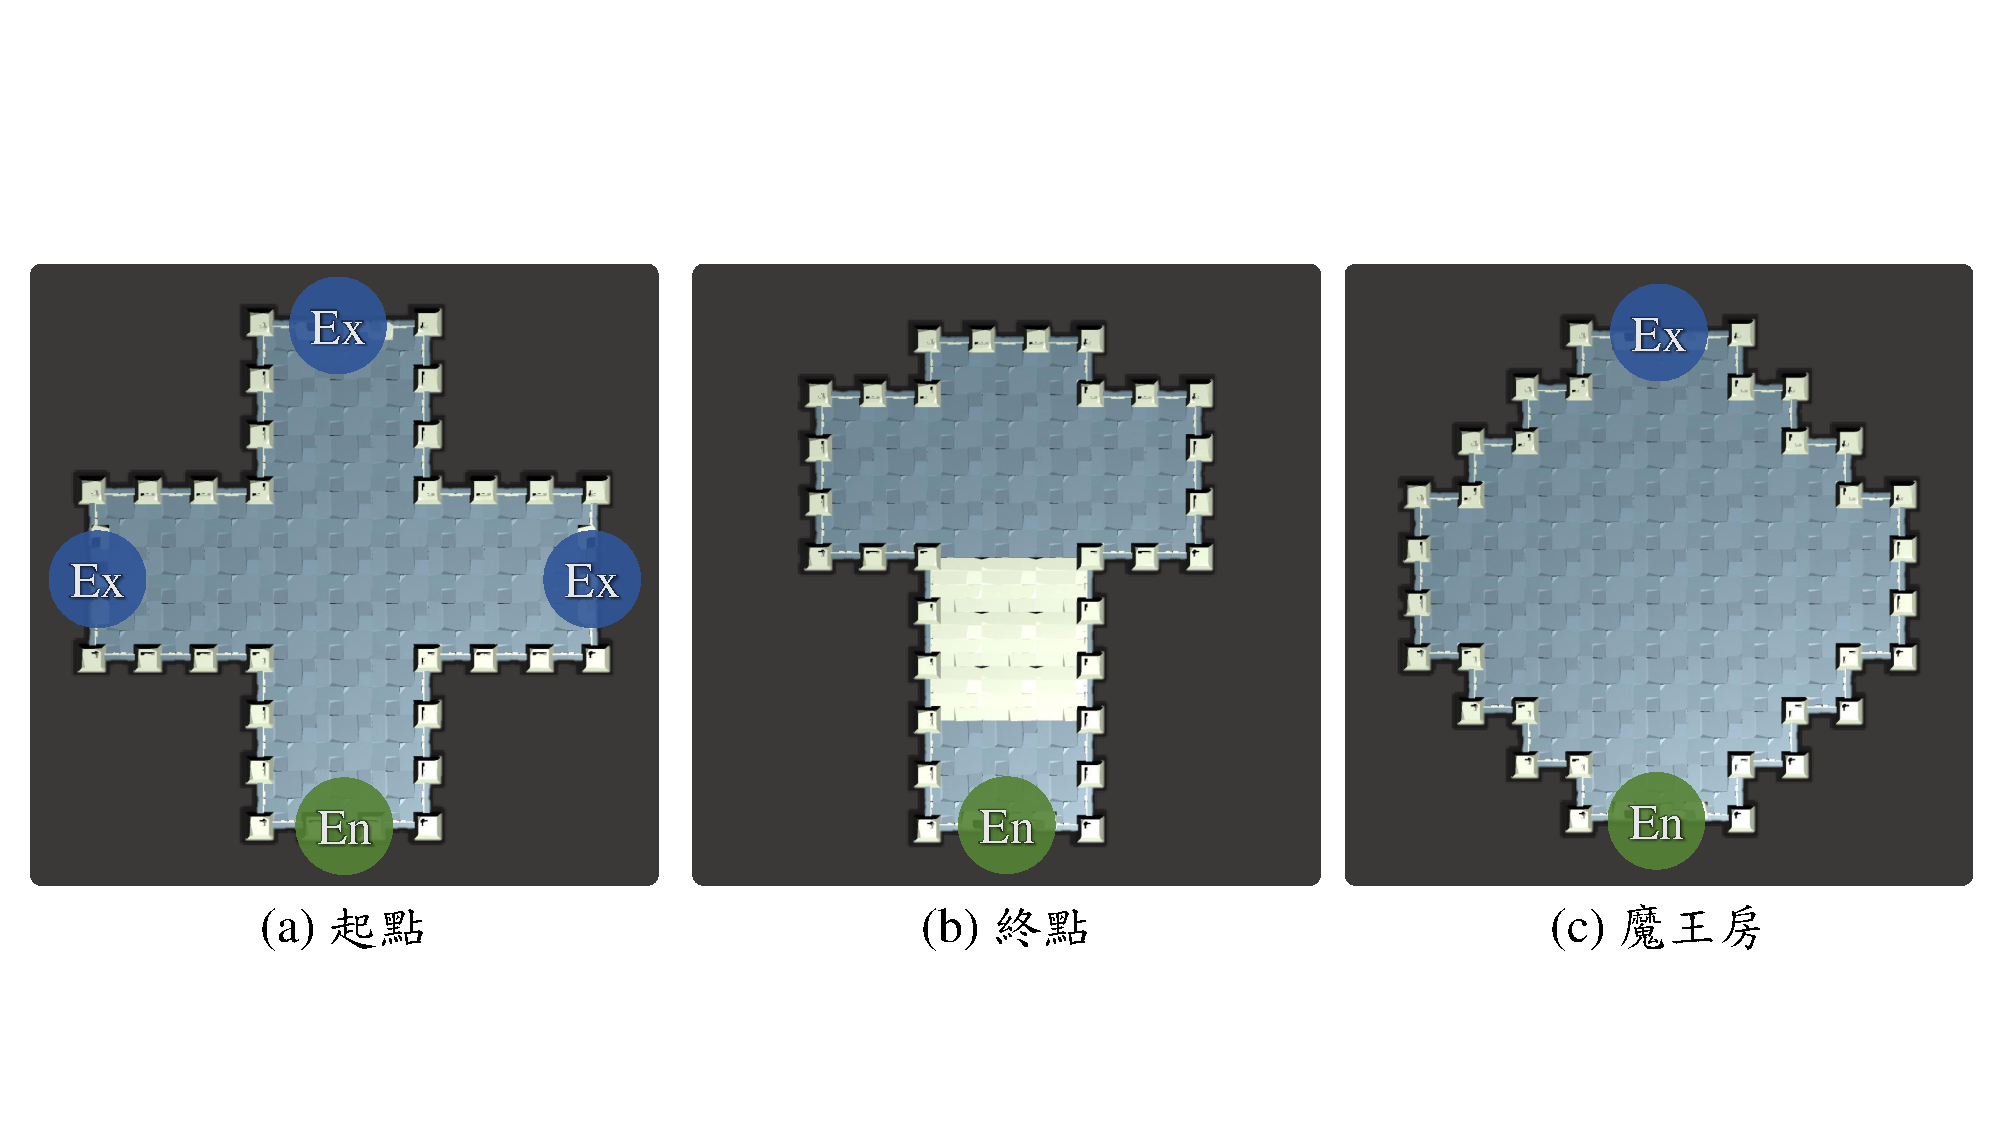
\includegraphics[width=1.0\textwidth]{figures/roomtype-mainpath-i.pdf}
    \caption{起點、終點與魔王房的房間容器結構}
    \label{fig:roomtype-mainpath-i}
  \end{center}
\end{figure}

\subsubsection{通道}
\label{sssec:method-spacepieces-types-path}

圖~\ref{fig:roomtype-mainpath-ii} 中,通道共有四種,隨著端點數量有等同的出口數量,因沒有入口識別物,便能夠以任一出口作為入口,搭配房間容器旋轉能達到共計 $11$ 種房型同構。圖~\ref{fig:roomtype-mainpath-ii} a 為 $I$ 型通道擁有二個出口,有二種同構結構;圖~\ref{fig:roomtype-mainpath-ii} b 為 $L$ 型通道擁有二個出口,有四種同構結構;圖~\ref{fig:roomtype-mainpath-ii} c 為 $T$ 型通道擁有三個出口,有四種同構結構;圖~\ref{fig:roomtype-mainpath-ii} d 為 $+$ 型通道擁有四個出口。

\begin{figure}[!htb]
  \begin{center}
    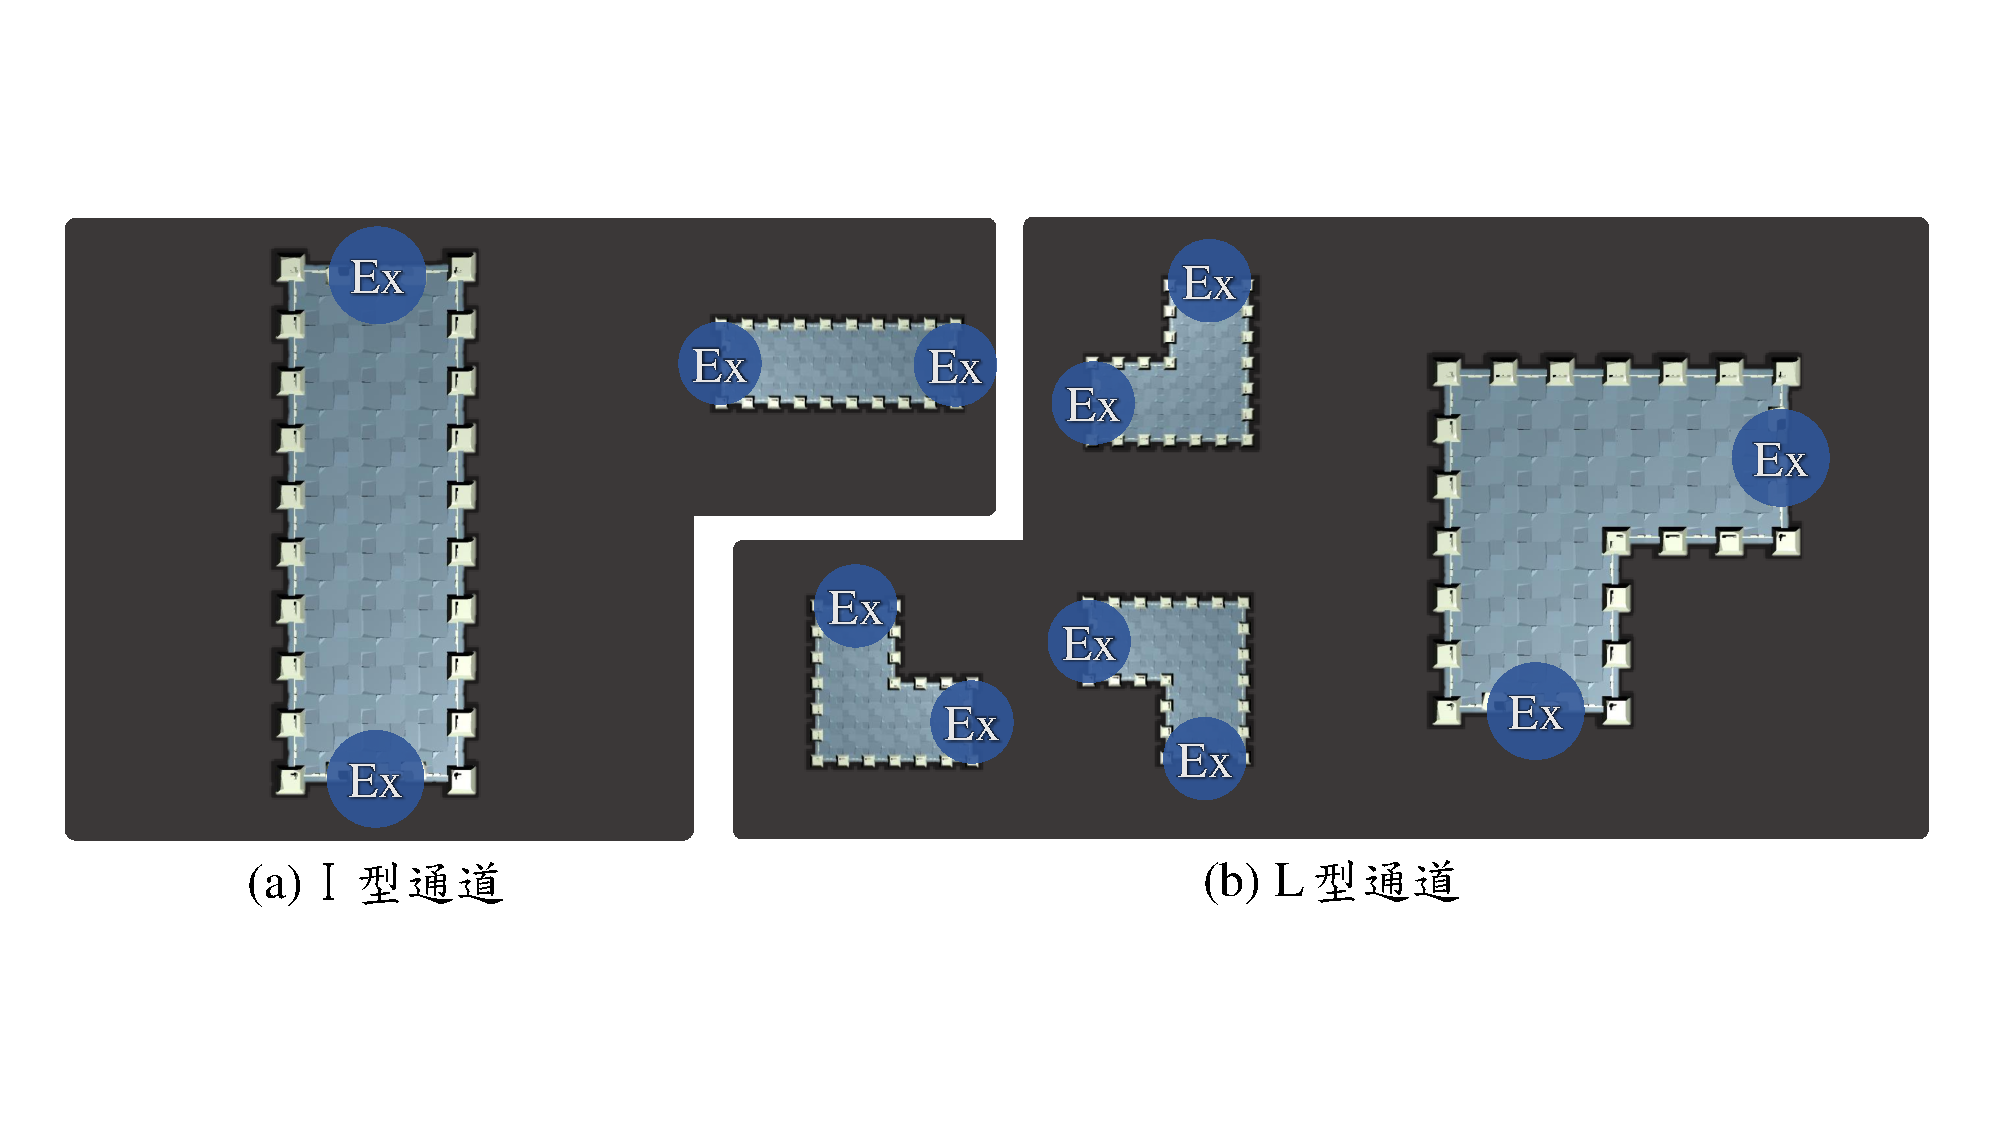
\includegraphics[width=1.0\textwidth]{figures/roomtype-mainpath-ii.pdf}
    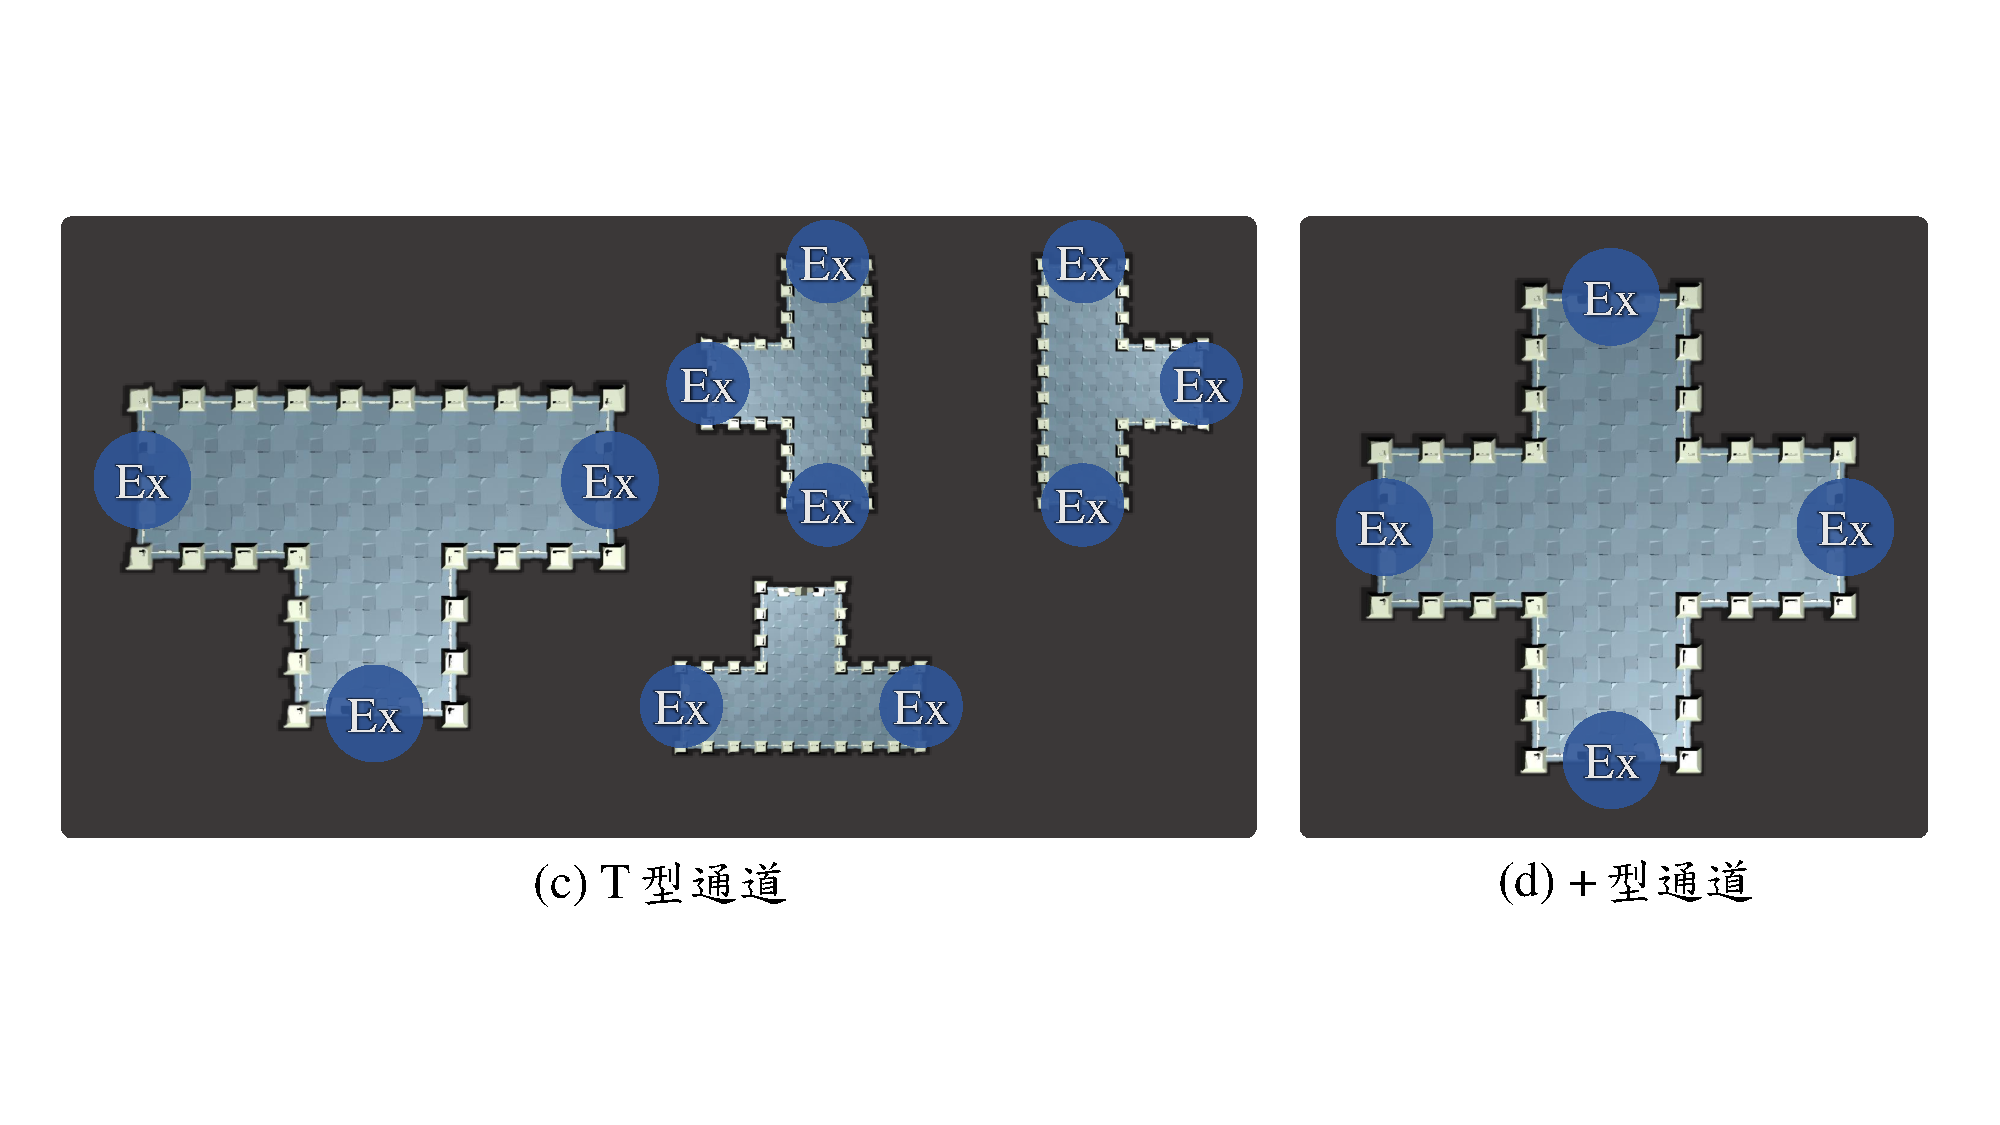
\includegraphics[width=1.0\textwidth]{figures/roomtype-mainpath-ii-.pdf}
    \caption{通道房間的房間容器結構與其同構示意}
    \label{fig:roomtype-mainpath-ii}
  \end{center}
\end{figure}

\subsubsection{石牆、秘密房、鎖、商店、寶藏房}
\label{sssec:method-spacepieces-types-special}

圖~\ref{fig:roomtype-special} a 為石牆擁有一個入口及一個出口,而出口的相同位置有石牆識別物;圖~\ref{fig:roomtype-special} b 為秘密房擁有一個入口,玩家能在該空間取得鑰匙識別物;圖~\ref{fig:roomtype-special} c 為鎖空間擁有一個入口及一個出口,在出口的相同位置有鎖識別物,玩家必須取得鑰匙方可通過;圖~\ref{fig:roomtype-special} d-e 為商店與寶藏房各擁有一個入口,玩家能夠在該房間觸發特殊事件。

\begin{figure}[!htb]
  \begin{center}
    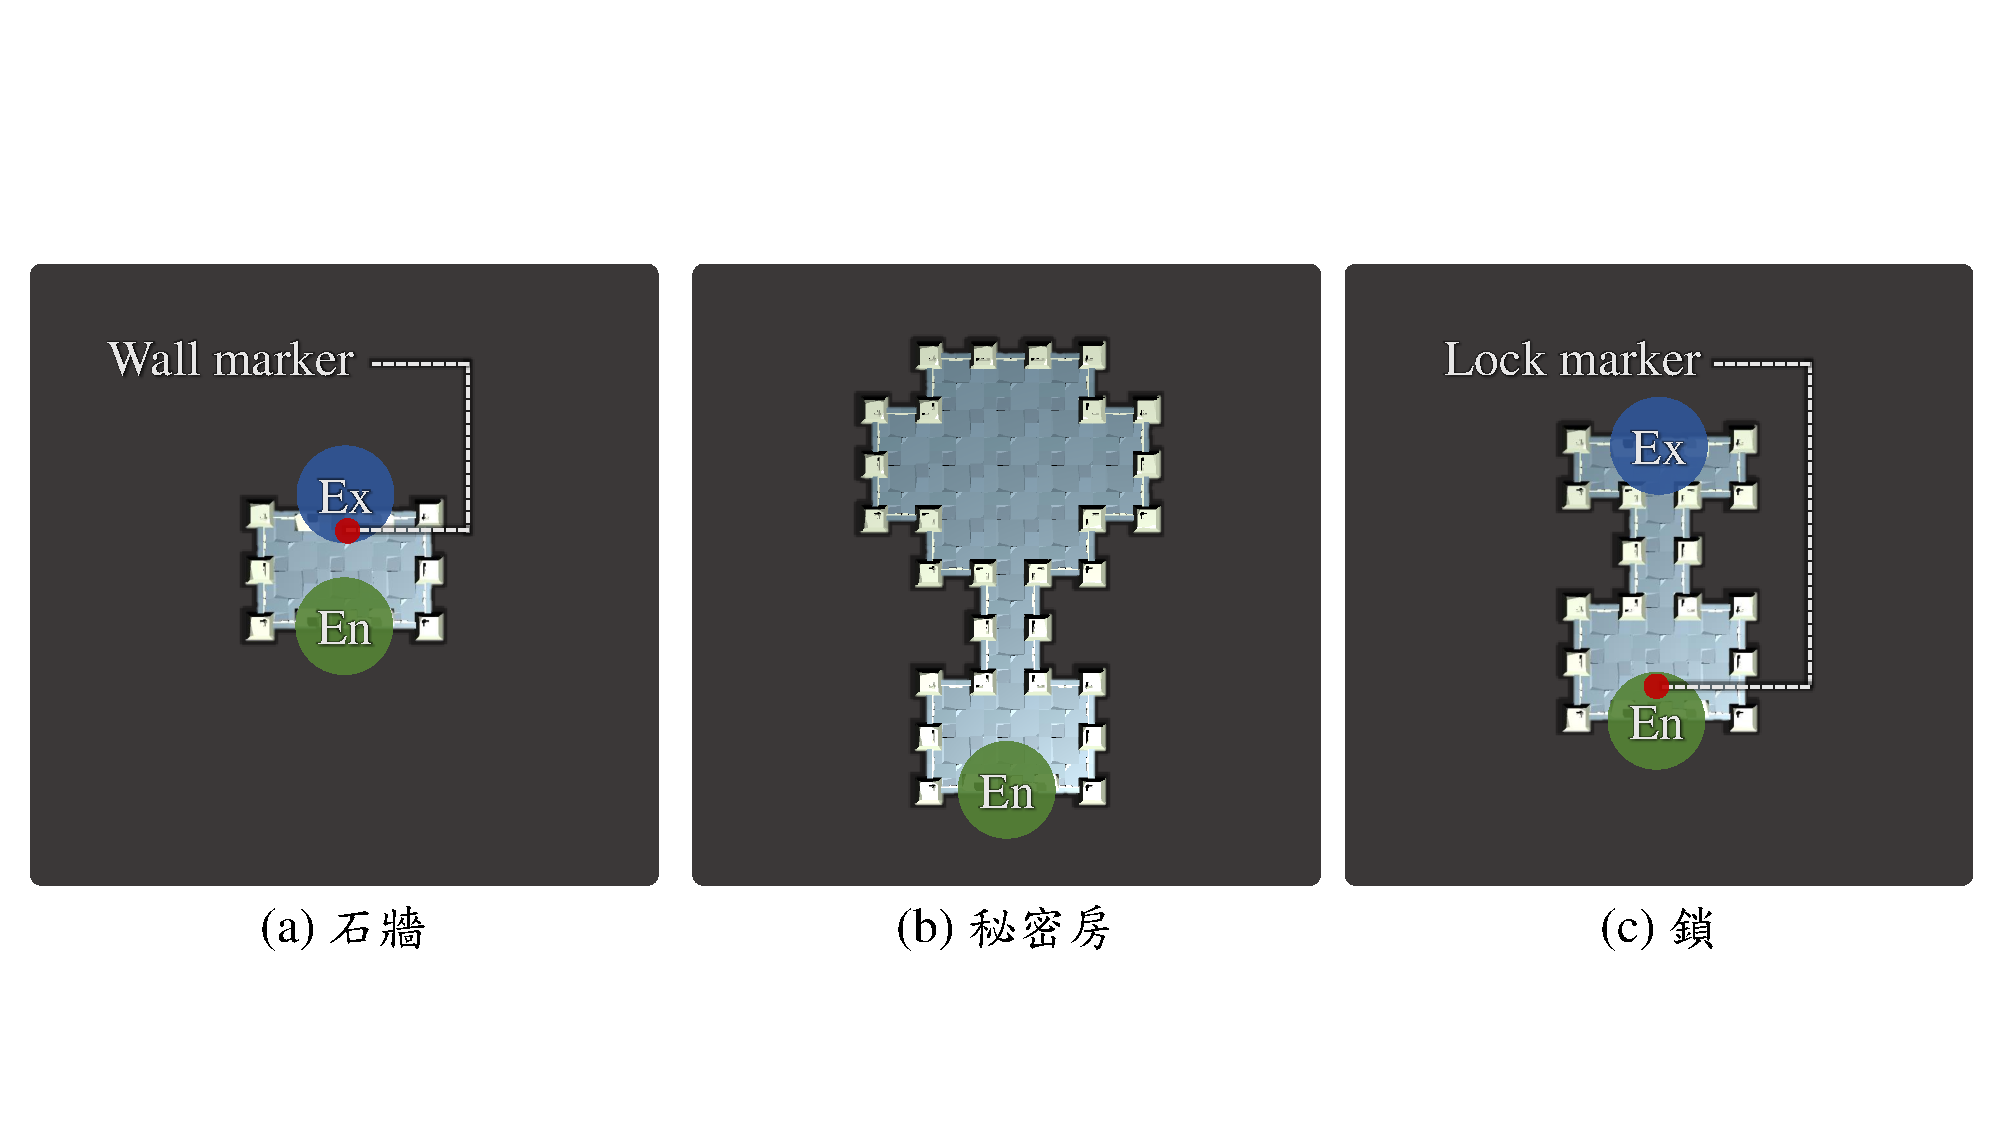
\includegraphics[width=1.0\textwidth]{figures/roomtype-special.pdf}
    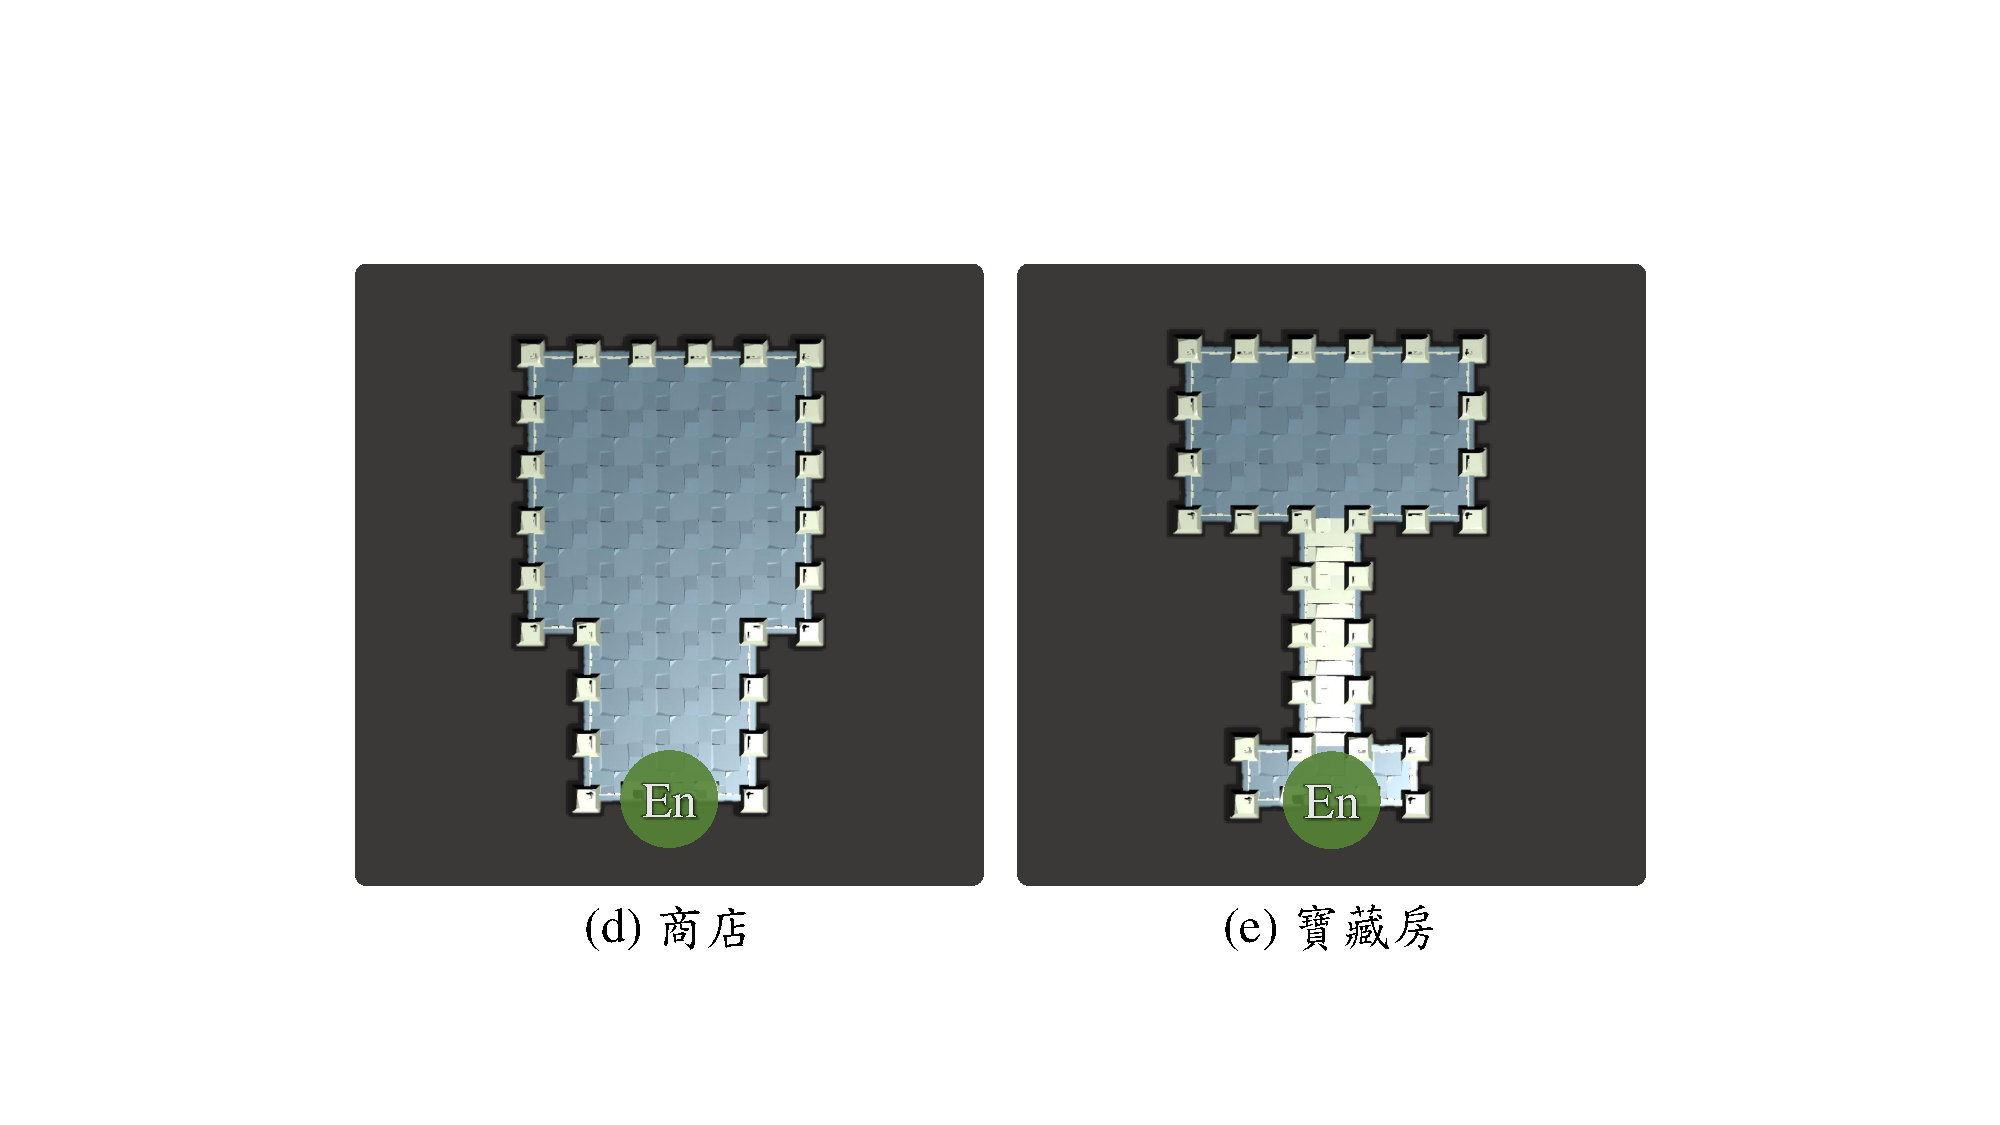
\includegraphics[width=1.0\textwidth]{figures/roomtype-special-.pdf}
    \caption{石牆、秘密房、鎖、商店與寶藏房的房間容器結構}
    \label{fig:roomtype-special}
  \end{center}
\end{figure}

\subsubsection{死路}
\label{sssec:method-spacepieces-types-wall}

在第~\ref{ssec:method-spacepieces-frommissiontospace} 小節中,為了要封閉剩餘的端點識別物所造成的空間開口,便需要無特殊功能的單一入口空間容器,見圖~\ref{fig:roomtype-wall}。

\begin{figure}[!htb]
  \begin{center}
    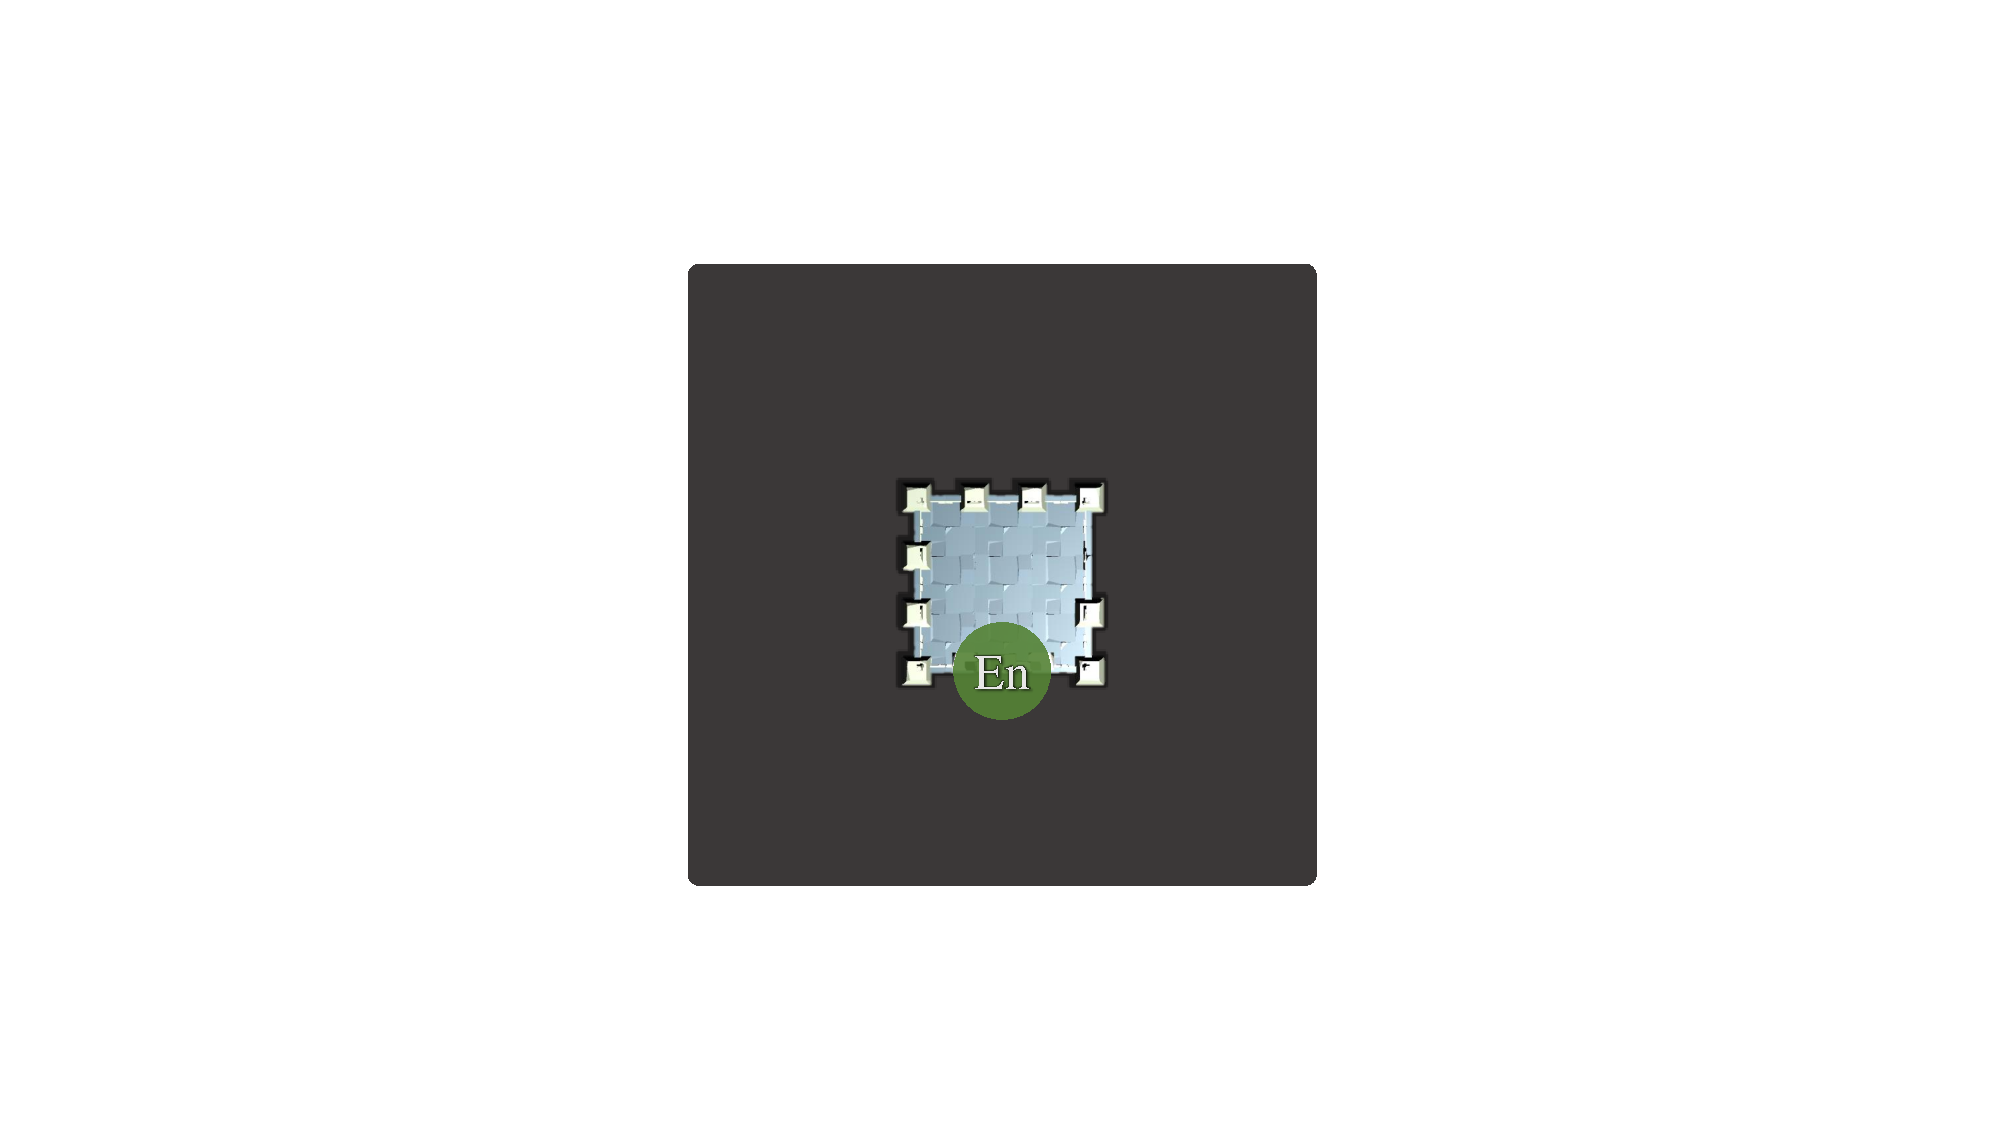
\includegraphics[width=1.0\textwidth]{figures/roomtype-wall.pdf}
    \caption{死路的房間容器結構}
    \label{fig:roomtype-wall}
  \end{center}
\end{figure}

\subsection{從任務圖轉為遊戲空間}
\label{ssec:method-spacepieces-frommissiontospace}

Joris Dormans 提到任務圖與空間圖應當是非常近似,甚至是二者同構~\cite{dormans2010adventures}。本小節將解釋 \textit{Dungeon Generator} 工具運行「將任務轉為空間的改寫系統」的流程,以及如何搭配任務圖的語法分析器。其一,藉由「建造方式表」能將任務圖轉換成有意義拓撲關係的遊戲空間;其二,利用「空間替換表」把前述遊戲空間不足之處補足。完成上述改寫系統進程後,便能夠輸出帶有任務邏輯的遊戲空間。演算法~\ref{alg:algorithm-mission-to-space-rewritesystem} 中,系統會遵循第~\ref{ssec:method-missiongrammars-graph} 小節產生的任務圖,以深度優先搜尋法遍歷任務圖,經過的源節點便從建造方式表中挑選出一個房間容器,逐一將各個終端節點轉換為實際空間,接著透過空間替換表,將場面上剩餘的端點識別物依序替換成對應房間容器,以完成遊戲空間之建置,相關演示可參考第~\ref{sssec:method-spacepieces-frommissiontospace-instruction}、~\ref{sssec:method-spacepieces-frommissiontospace-replacement} 二小節,將會逐一介紹演算法~\ref{alg:algorithm-mission-to-space-rewritesystem} 的實際應用流程。

\begin{algorithm}[!htb]
    \caption{RewriteSystem2 - 改寫系統(任務轉換空間)}
    \label{alg:algorithm-mission-to-space-rewritesystem}
    \begin{algorithmic}[1]
        \Require
            \Statex $graph$ is $MissionGraph$.
            \Statex $seed$ is the random seed.
        \Ensure
            \ForAll {$node\in graph$}:                                              \Comment{Instrcution,第~\ref{sssec:method-spacepieces-frommissiontospace-instruction} 小節}
                \State {$volume$ = GetVolumeFromInstructionTable($node$, $seed$)}   \Comment{參照表~\ref{tbl:mission-to-space-instruction}}
                \State {$isSucceed$ = SetVolumeToSpace($volume$, $seed$)}           \Comment{return $true$ or $false$}
                \If {$isSucceed$ is $false$}
                    \Return {$false$}
                \EndIf
            \EndFor
            \ForAll {$marker\in ConnectionsInGraph$}:                               \Comment{Replacement,第~\ref{sssec:method-spacepieces-frommissiontospace-replacement} 小節}
                \State {$volume$ = GetVolumeFromReplacementTable($marker$, $seed$)} \Comment{參照表~\ref{tbl:mission-to-space-replace}}
                \State {$isSucceed$ = SetVolumeToSpace($volume$, $seed$)}           \Comment{return $true$ or $false$}
                \If {$isSucceed$ is $false$}
                    \Return {$false$}
                \EndIf
            \EndFor \\
            \Return {$true$}                                                        \Comment{Successfully generated a game space}
    \end{algorithmic}
\end{algorithm}

\subsubsection{建造方式}
\label{sssec:method-spacepieces-frommissiontospace-instruction}

為從已生成完畢的任務圖進而衍生出遊戲空間,在創建的房間容器會對應一任務符號表當中的終端符 (terminal symbols),稱作為建造方式 (building instruction)。本小節會利用第~\ref{ssec:method-missiongrammars-alphabet} 小節的任務符號表,過濾出終端節點並逐一對應至第~\ref{ssec:method-spacepieces-types} 小節的房間容器,見表~\ref{tbl:mission-to-space-instruction}。每一個終端節點都必須對應一個以上的房間容器,房間容器不允許被重複使用在不同的終端節點上。

\setlength\LTcapwidth{\linewidth}
\begin{longtable}{
    | >{\centering\arraybackslash} m{1.0cm}
    | >{\centering\arraybackslash} m{3.5cm}
    | >{} m{1.0cm}
    | >{\centering\arraybackslash} m{1.0cm}
    | >{\centering\arraybackslash} m{3.5cm} | }
  \caption{建造方式表,任務終端節點與房間容器對應之範例}\label{tbl:mission-to-space-instruction} \\
  \cline{1-2}\cline{4-5}
  節點 & 對應之房間容器 &  & 節點 & 對應之房間容器 \\
  \cline{1-2}\cline{4-5}
  \endfirsthead
  \multicolumn{5}{c}%
  {\tablename\ \thetable\ -- \textit{接續前頁面}} \\
  \cline{1-2}\cline{4-5}
  節點 & 對應之房間容器 &  & 節點 & 對應之房間容器 \\
  \cline{1-2}\cline{4-5}
  \endhead
  \multicolumn{5}{r}{\textit{接續下頁面}} \\
  \endfoot
  \endlastfoot
  \missionalphabetnode{t-entrance}{10mm}
    & \missioninstruction{instruction-01}
    &
    & \missionalphabetnode{t-goal}{10mm}
    & \missioninstruction{instruction-02}
    \\\cline{1-2}\cline{4-5}
  \missionalphabetnode{t-boss}{10mm}
    & \missioninstruction{instruction-03}
    &
    & \missionalphabetnode{t-normal}{10mm}
    & \missioninstruction{instruction-04}
    \\\cline{1-2}\cline{4-5}
  \missionalphabetnode{t-normal}{10mm}
    & \missioninstruction{instruction-05}
    &
    & \missionalphabetnode{t-normal}{10mm}
    & \missioninstruction{instruction-06}
    \\\cline{1-2}\cline{4-5}
  \missionalphabetnode{t-normal}{10mm}
    & \missioninstruction{instruction-07}
    &
    & \missionalphabetnode{t-bomb}{10mm}
    & \missioninstruction{instruction-08}
    \\\cline{1-2}\cline{4-5}
  \missionalphabetnode{t-secret}{10mm}
    & \missioninstruction{instruction-09}
    &
    & \missionalphabetnode{t-lock}{10mm}
    & \missioninstruction{instruction-10}
    \\\cline{1-2}\cline{4-5}
  \missionalphabetnode{t-shop}{10mm}
    & \missioninstruction{instruction-11}
    &
    & \missionalphabetnode{t-treasure}{10mm}
    & \missioninstruction{instruction-12}
    \\\cline{1-2}\cline{4-5}
\end{longtable}

圖~\ref{fig:mission-to-space-instruction-flow} a 為使用第~\ref{ssec:method-missiongrammars-rules} 小節的任務規則表(表~\ref{tbl:missiongrammars-rules-linear-example}-~\ref{tbl:missiongrammars-rules-nonlinear-example3})所生成的任務圖,該階段採用的亂數種子為 $0$。本階段中,依照演算法~\ref{alg:algorithm-mission-to-space-rewritesystem} - 改寫系統(任務轉換空間),並且結合表~\ref{tbl:mission-to-space-instruction} 的建造方式表,將任務圖轉換為遊戲空間。圖~\ref{fig:mission-to-space-instruction-flow} b 可見,第一個節點起點 (entrance\missionalphabetnode{t-entrance}{5mm}) 直接對應到「起點房間容器」,而起點房間容器中擁有三個出口端點,系統將會亂數隨機一個出口端點進行後續房間生成,根據深度優先搜尋法下一個遍歷的節點為第二行的一般房 (normal\missionalphabetnode{t-normal}{5mm}),接著從建造方式表中過濾出能夠使用的四種「通道房間容器」,由系統亂數決定本次採用的房間容器後,將預計新增的房間容器之起點與前一步驟決定的出口端點進行房間容器連接,下一回合將從新增的房間容器重複前述之步驟。依照上述之步驟,改寫系統(任務轉換空間)完整遍歷所有的任務節點後,便能夠完成任務轉換空間的動作,結果可參考圖~\ref{fig:mission-to-space-instruction-result}。

進行疊代的過程時,以下幾種情形,疊代生成將會失敗:當任務圖節點的子節點數量大於對應房間容器的出口數量;當新生長的房間容器於其它房間容器發生碰撞。因此,若有以上違例情況,關卡設計師必須修正其關卡設計,如調整房間容器之格局或更換一筆亂數種子,並重新執行前述步驟。

\begin{figure}[!htb]
  \begin{center}
    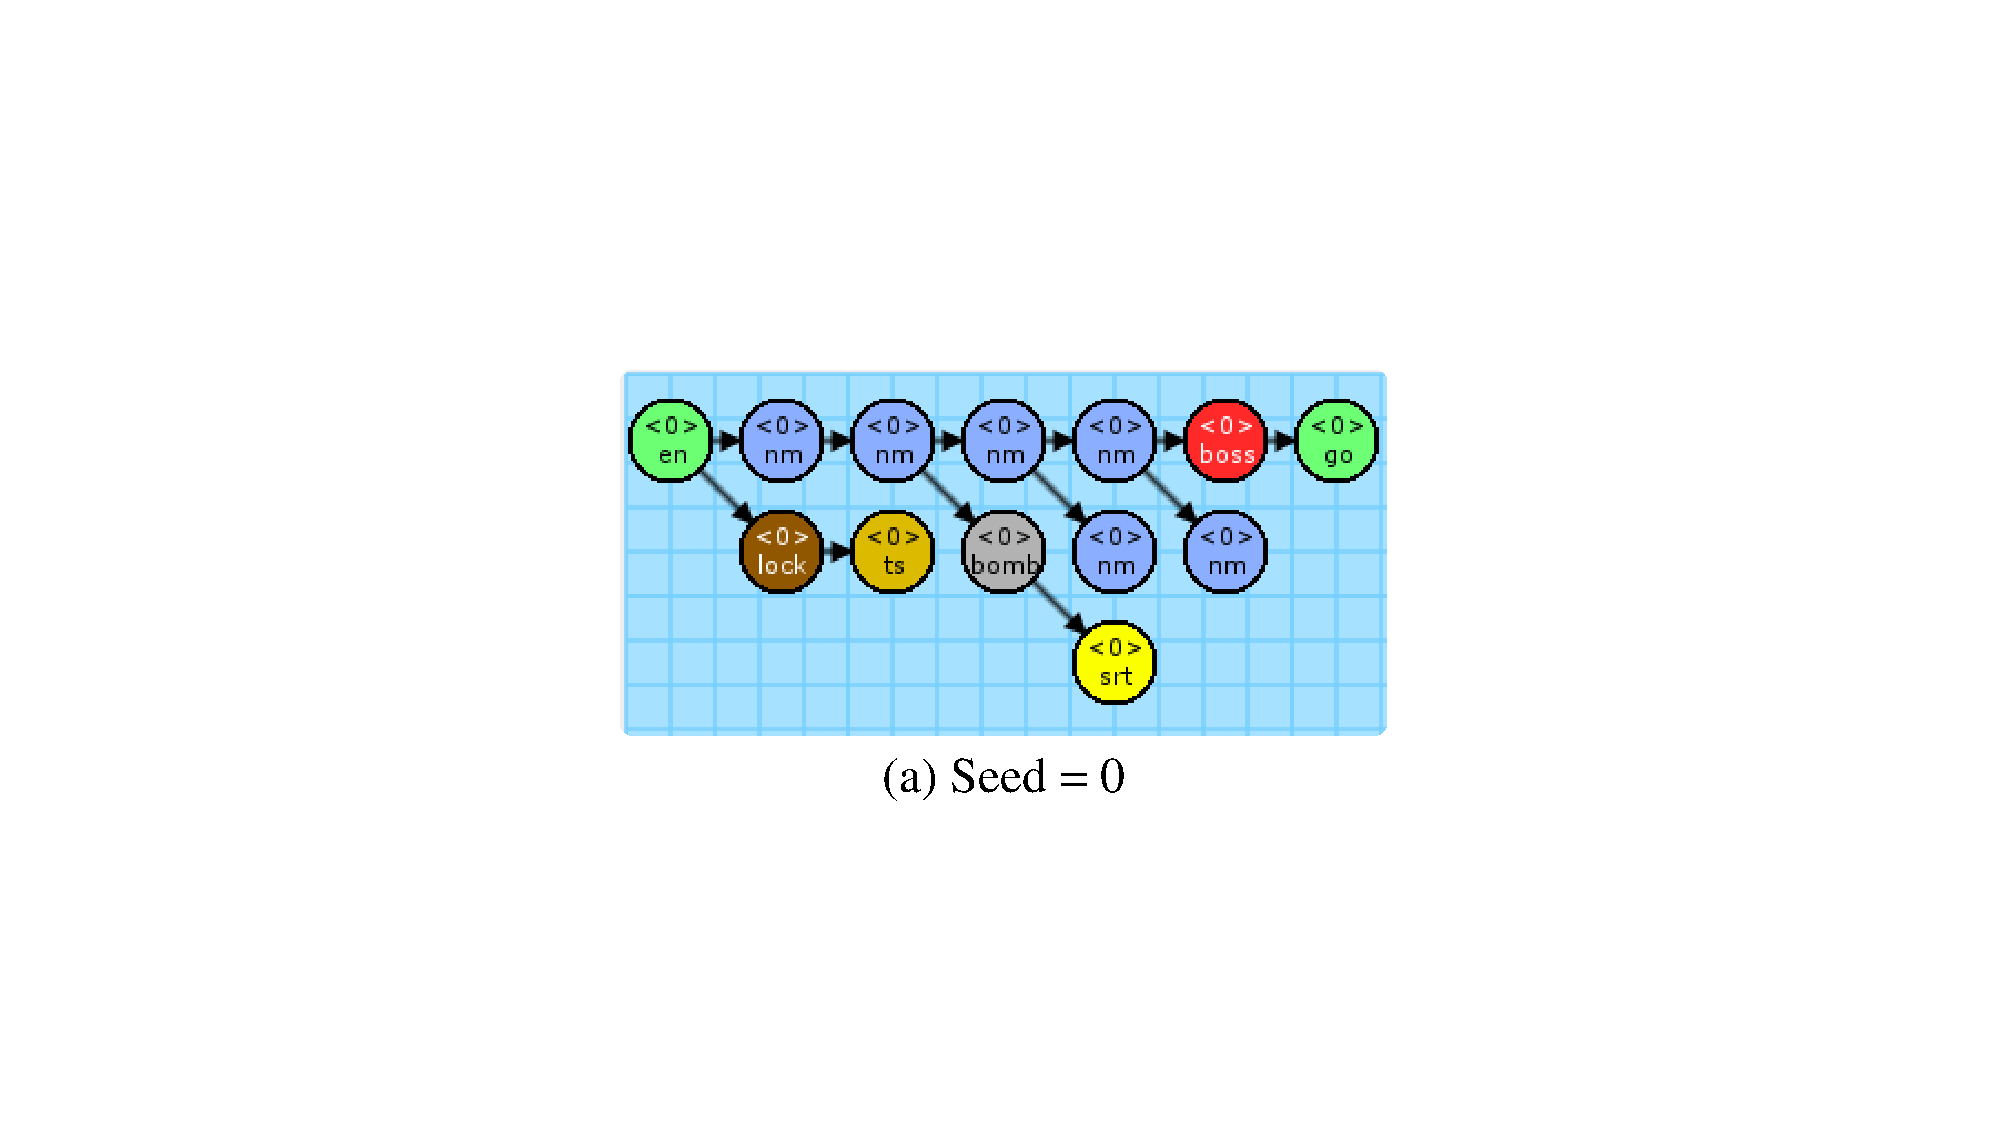
\includegraphics[width=1.0\textwidth]{figures/mission-to-space-instruction-flow.pdf}
    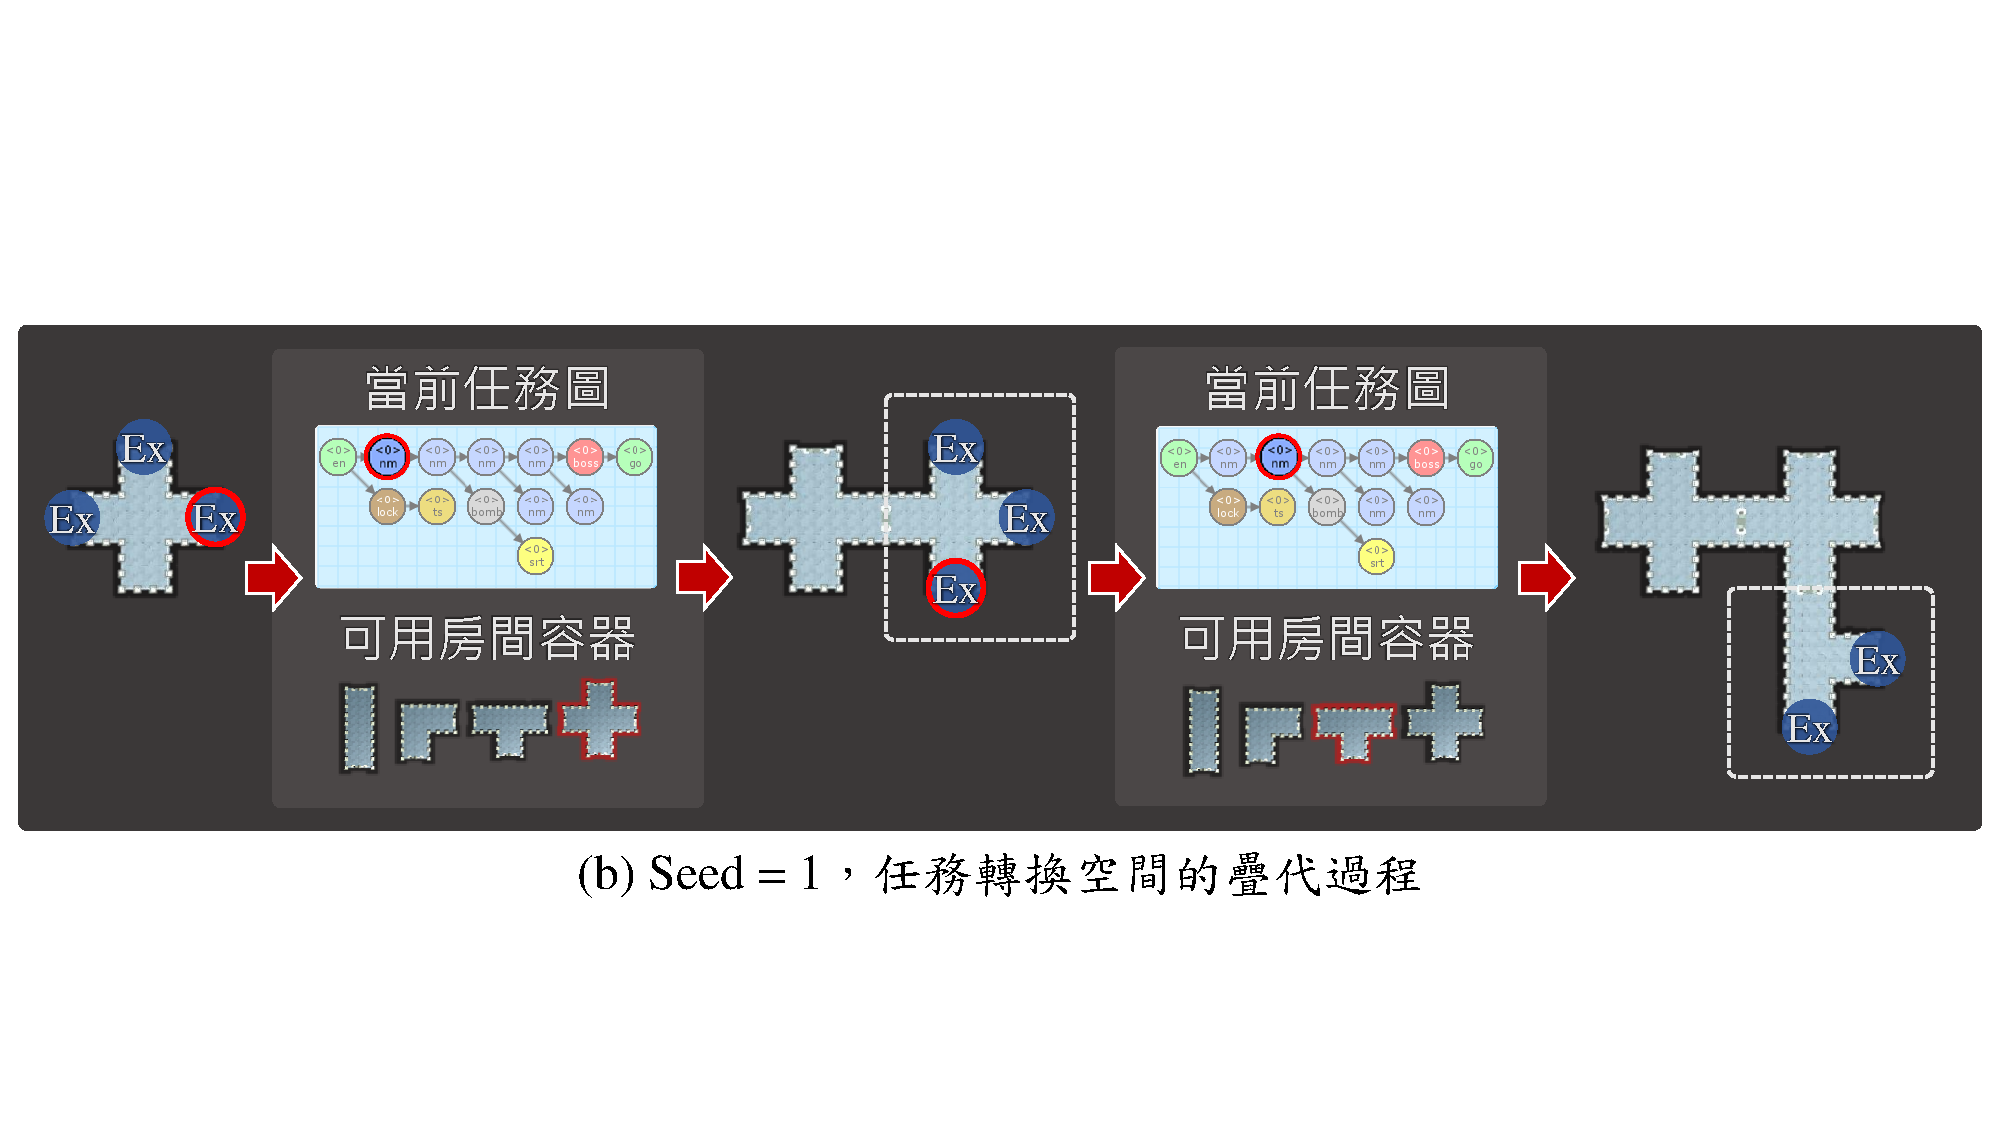
\includegraphics[width=1.0\textwidth]{figures/mission-to-space-instruction-flow-.pdf}
    \caption{建造方式的疊代生成過程} 
    \label{fig:mission-to-space-instruction-flow}
  \end{center}
\end{figure}

基於建造方法的對應紀錄,給予一亂數種子能夠確保能夠對應到一固定空間。當終端節點對應到複數房間容器時,亂數種子將影響從多個房間容器之間的順序。若生成過程中,該房間容器擁有多個出口,亦是參照亂數種子決定調用出口生成之順序,見圖~\ref{fig:mission-to-space-instruction-result}。

\begin{figure}[!htb]
  \begin{center}
    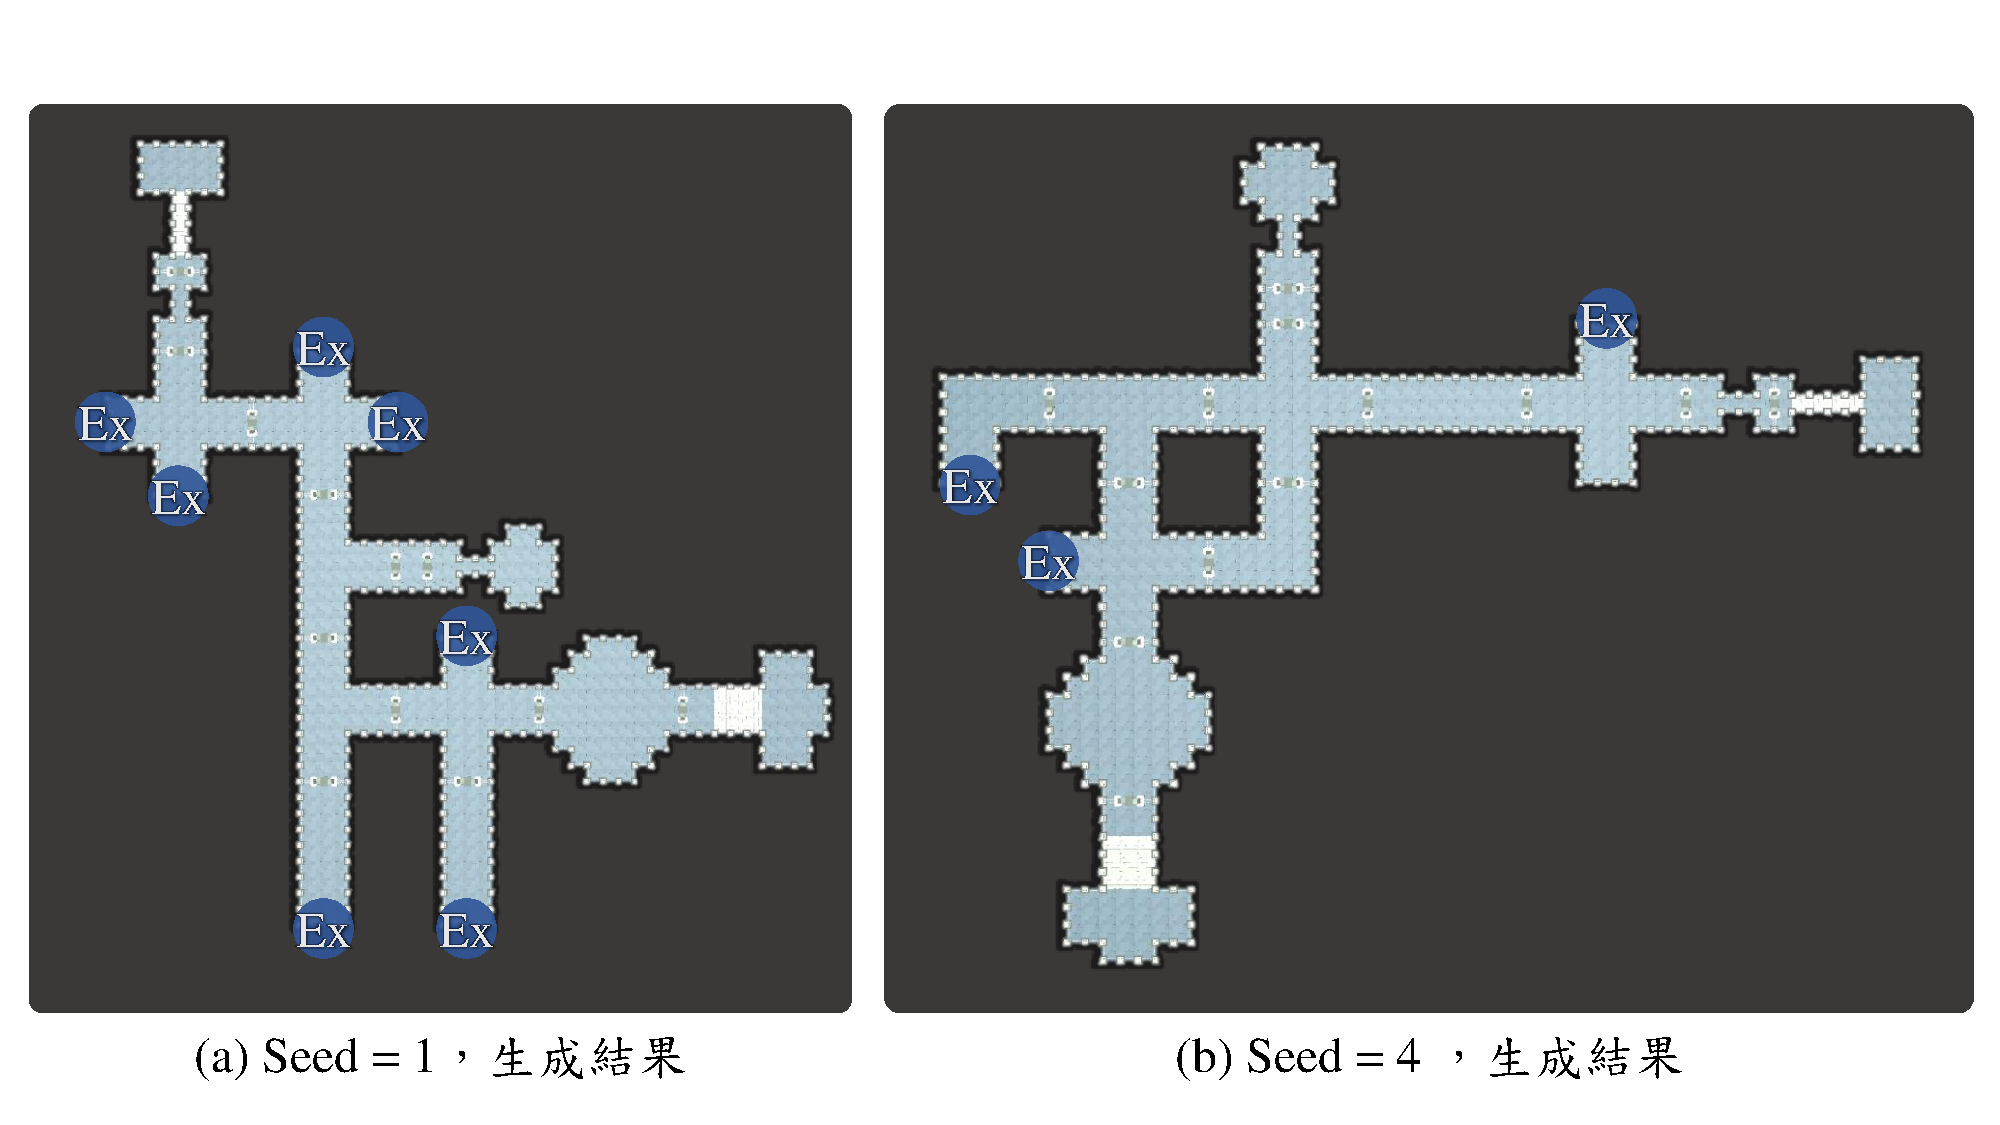
\includegraphics[width=1.0\textwidth]{figures/mission-to-space-instruction-result.pdf}
    \caption{已疊代生成的任務圖,不同亂數種子轉換為對應結果的遊戲空間} 
    \label{fig:mission-to-space-instruction-result}
  \end{center}
\end{figure}

\subsubsection{剩餘空間替換}
\label{sssec:method-spacepieces-frommissiontospace-replacement}

一個端點識別物能夠對應複數個房間容器,房間容器能夠重複被不同的端點識別物所對應。第~\ref{ssec:method-spacepieces-connections} 小節,介紹端點識別物時,曾提及到遊戲設計師能夠自由擴充出口識別物的種類。在此為簡化範例,表~\ref{fig:mission-to-space-instruction-result} 採用預設之單一出口識別物,而這項出口識別物將對應圖~\ref{fig:roomtype-wall} 的死路房間容器,左側為端點識別物之種類,右側為所對應的房間容器。

\begin{table}[!htb]
  \centering
  \caption{空間替換表,出口端點與房間容器對應之範例}
  \label{tbl:mission-to-space-replace}
  \bigskip
  \begin{tabular}{
    | >{\centering\arraybackslash} m{1.5cm}
    | >{\centering\arraybackslash} m{3.5cm} | }
    \hline
    \multicolumn{1}{ |c| }{端點}
      & \multicolumn{1}{ c| }{對應之房間容器} \\\hline
    \begin{minipage}{.3\textwidth}
\includegraphics[width=15mm]{figures/mission-grammars-ins-rep/replacement-l-01.png}\end{minipage}
      & \begin{minipage}{.3\textwidth}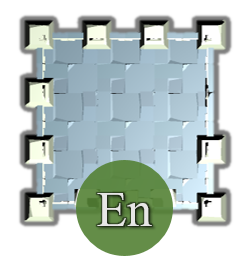
\includegraphics[width=35mm]{figures/mission-grammars-ins-rep/replacement-r-01.png}\end{minipage}
      \\\hline
  \end{tabular}
\end{table}

在圖~\ref{fig:mission-to-space-instruction-result} 可觀察到,經過建造方式的遊戲空間仍會遺留部分的端點識別物,為了將其延伸或予以封閉,本小節將進行替換 (replacement) 使遊戲空間趨於完整,見圖~\ref{fig:mission-to-space-replacement-result}。若增加空間替換表其對應的選項,便能創造出主線外的分支結構。

\begin{figure}[!htb]
  \begin{center}
    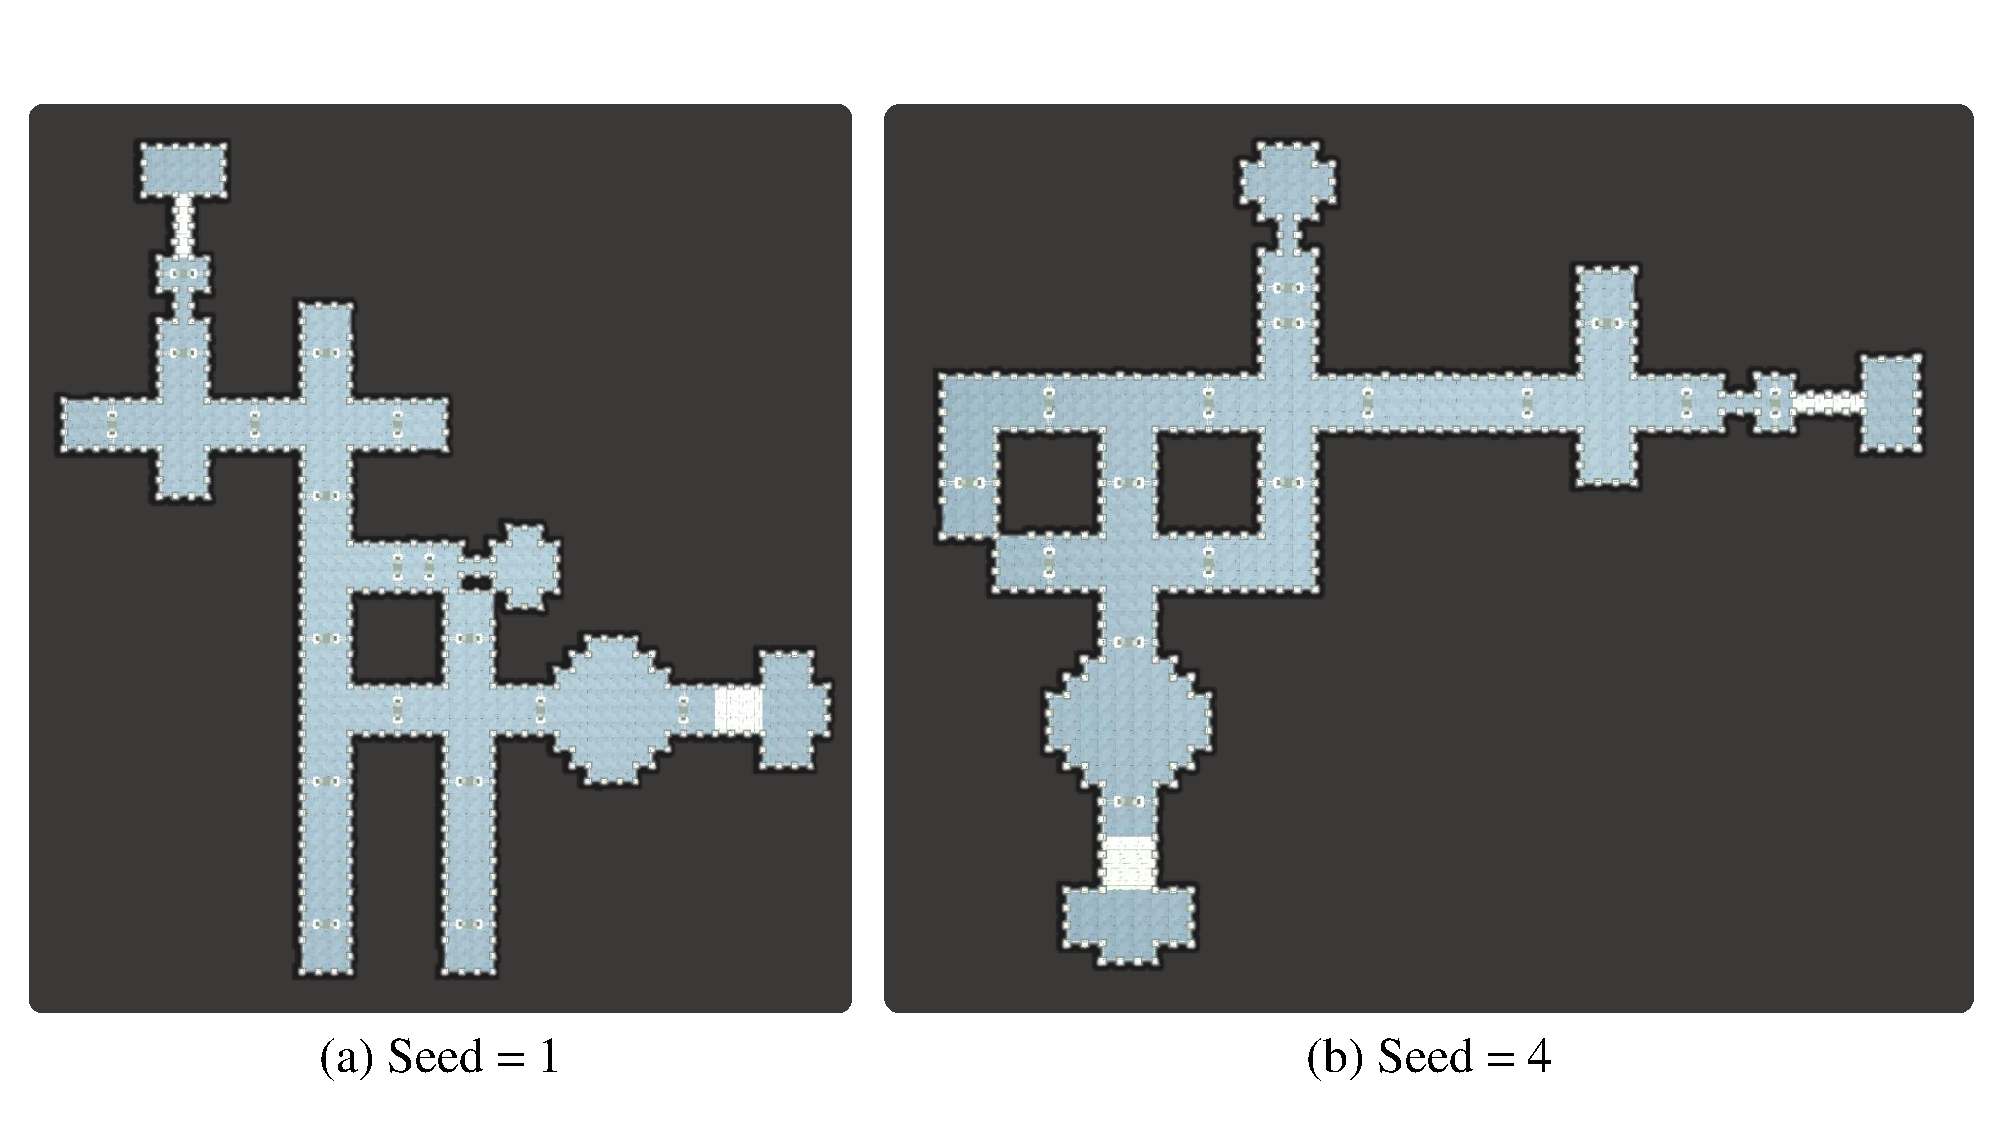
\includegraphics[width=1.0\textwidth]{figures/mission-to-space-replacement-result.pdf}
    \caption{經過剩餘空間替換後的完整遊戲空間} 
    \label{fig:mission-to-space-replacement-result}
  \end{center}
\end{figure}

% Clean the page after this section.
\clearpage

\section{地圖片段}
\label{sec:method-segments}

為了將第~\ref{ssec:relatedworks-proceduralgamepatterns} 小節提及的程序化遊戲物件擺放技術付諸實現,構築出遊戲內部的複雜系統,讓玩家體驗到突現型 (emergence) 的遊玩機制,我們將延續上一節的遊戲關卡結構,參考 Antonios Liapis 提出的地圖片段演化方法~\cite{liapis2017multi},令地圖片段為房間容器,並進行改良以合適我方實驗環境。

圖~\ref{fig:segments-with-ga} 介紹地圖片段的演化流程。第一步驟,基於第~\ref{ssec:method-segments-gene} 小節中定義的基因結構,產生初始父母代族群時,讓全部的基因先預設為空磚;第二步驟,透過適應性函數計算各個體的適應值 (fitnesses),完整的適應性函數在第~\ref{ssec:method-segments-fitnesses} 小節中說明;第三步驟將會從族群中挑選最優異的兩個父母染色體,高機率進行交配,若無進行交配將會將子代沿用父母代的基因;第四步驟有低機率讓衍生的子代進行突變;第五步驟以新的衍生子代取代舊有的父母代族群;第六步驟會檢查是否達到終止條件,若尚未滿足終止條件,便會回到第二步驟,直到輸出最適解。前述之交配、突變事件的機率與其方法屬於實驗變因,將在第~\ref{cha:experiment} 章進行定義與相關釋義。

\begin{figure}[!htb]
  \begin{center}
    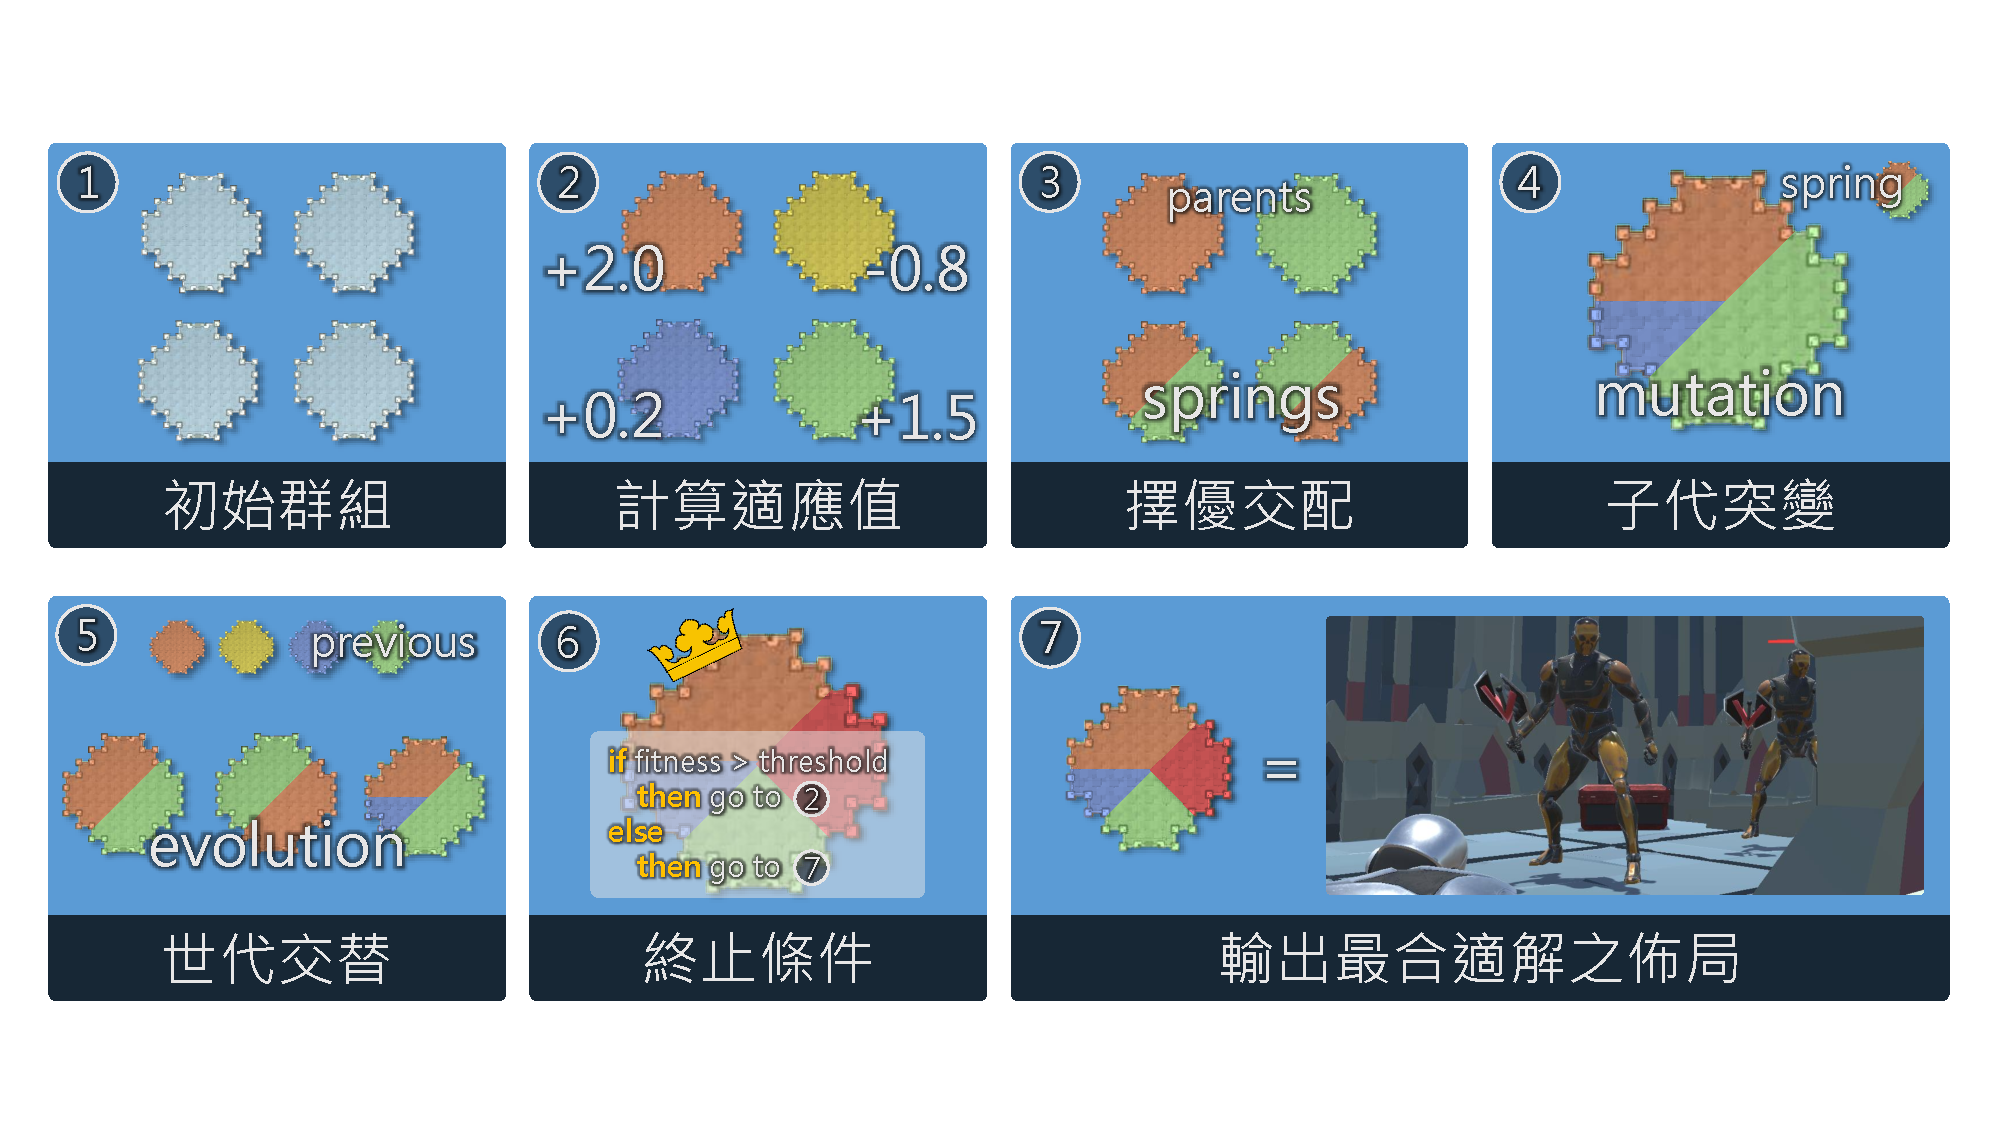
\includegraphics[width=1.0\textwidth]{figures/segments-with-ga.pdf}
    \caption{房間容器採取基因演算法之演化流程} 
    \label{fig:segments-with-ga}
  \end{center}
\end{figure}

\subsection{基因的儲存結構}
\label{ssec:method-segments-gene}

圖~\ref{fig:segments-gene-expression} a 是遊戲物件的表型 (phenotype),為基因演算法中的個體單位,房間容器能夠存放數種遊戲物件,分別為空磚 (Empty)、敵人磚 (Enemy)、寶箱磚 (Treasure) 與陷阱磚 (Trap),圖中帶有編號的位置意指著該座標能夠擺放遊戲物件,且玩家角色能夠在該座標通過;遊戲物件的擺放位置為個體的染色體 (chromosome),以一維陣列之基因序列表示,見圖~\ref{fig:segments-gene-expression} b;基因序列中的基因,會存放該座標的相對位置與遊戲物件類型,見圖~\ref{fig:segments-gene-expression} c。同一個房間容器會擁有許多不同的個體,這些個體的集合便是族群 (population)。

\begin{figure}[!htb]
  \begin{center}
    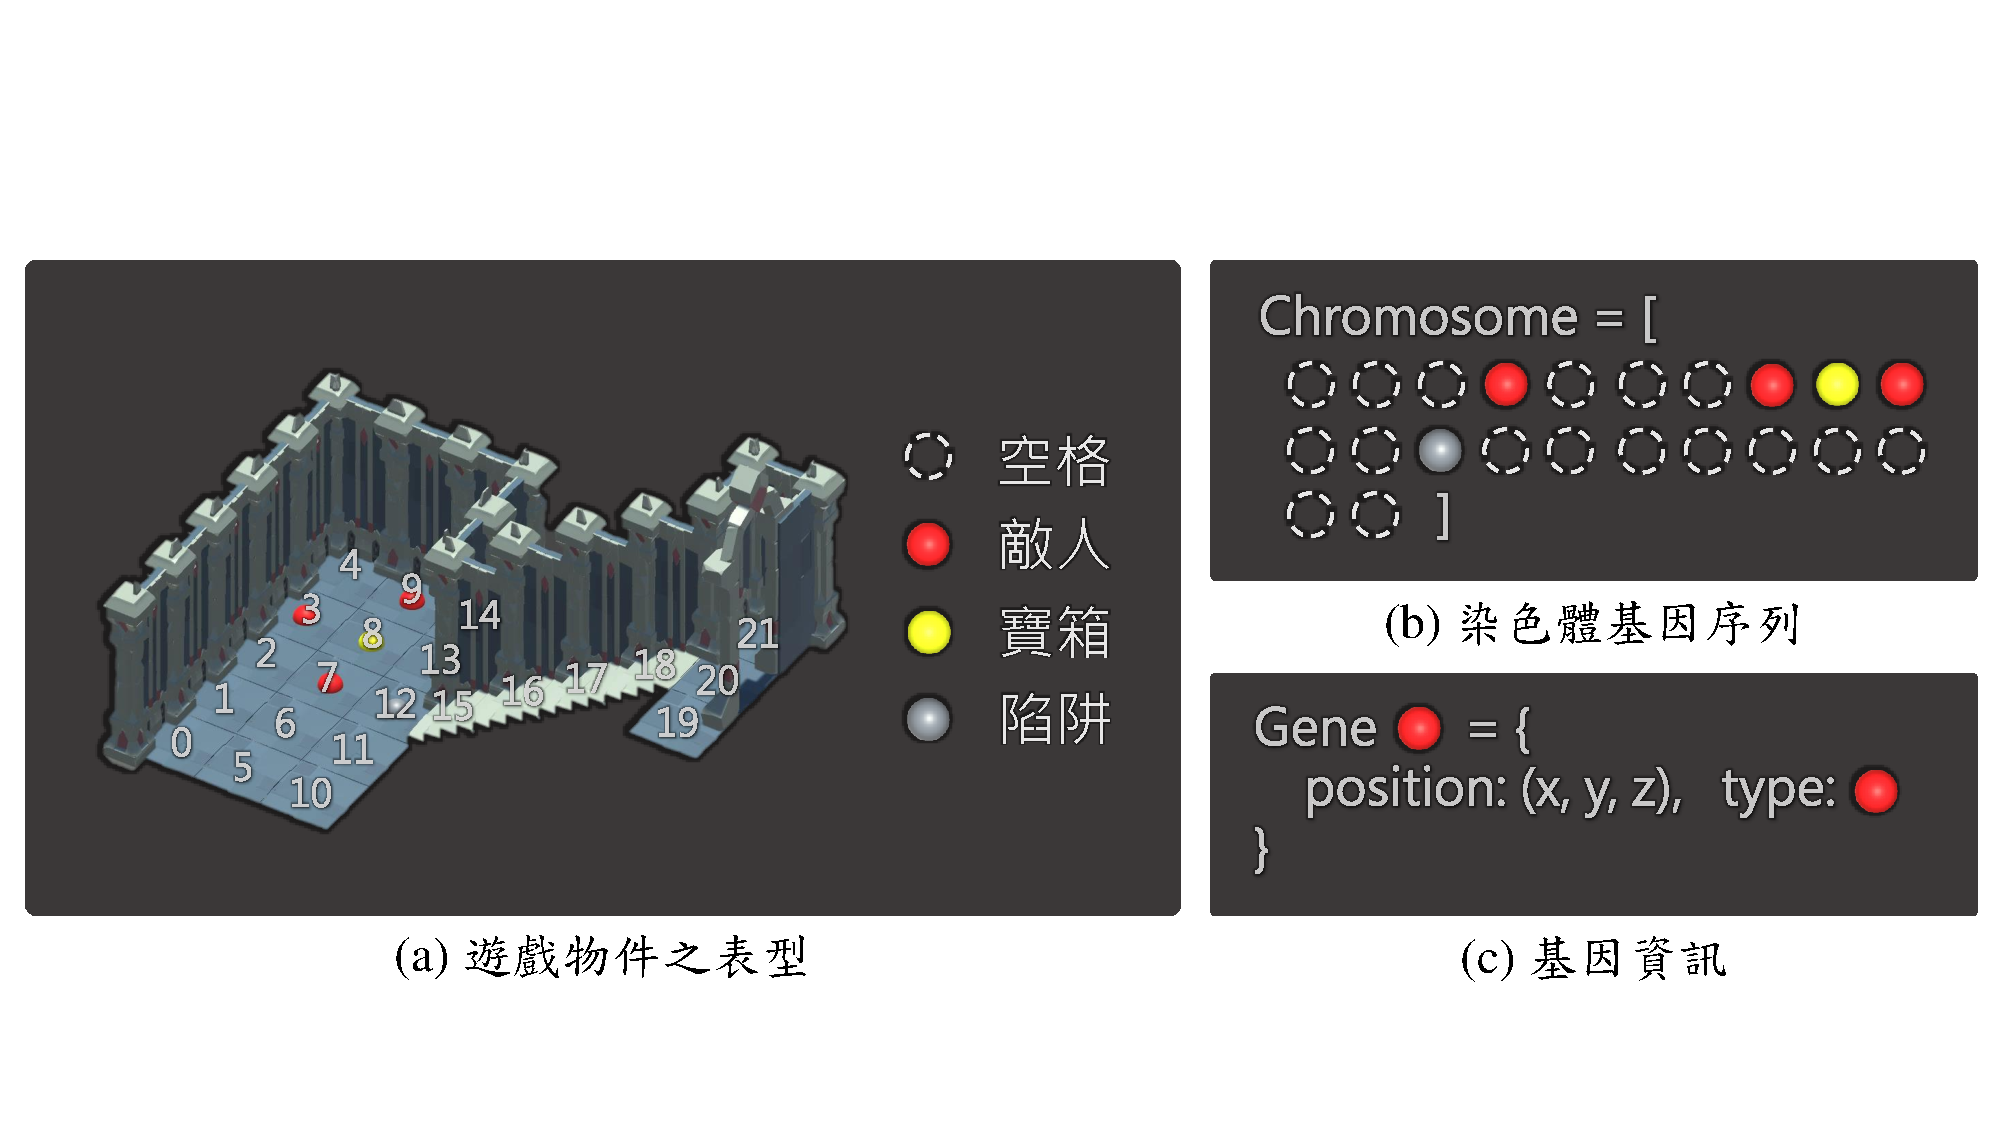
\includegraphics[width=1.0\textwidth]{figures/segments-gene-expression.pdf}
    \caption{房間容器以遊戲物件的佈局方式作為染色體}
    \label{fig:segments-gene-expression}
  \end{center}
\end{figure}

\subsection{演化之適應性函數}
\label{ssec:method-segments-fitnesses}

動作冒險遊戲 (A-AVG)、動作角色扮演遊戲 (A-RPG) 等類型遊戲,多可見一些制式化遊戲物件的搭配組合,Alexander Baldwin 認為遊戲物件組合的細觀特徵 (Meso-Patterns) 需要有檢測其品質的方法~\cite{baldwin2017mixed}。我們嘗試汲取出多項遊玩特徵並參數化公式,作為評估關卡品質的指標之一。

於前處理階段時,圖~\ref{fig:decorations-with-directions} 中顯示的地面、階梯裝飾物屬於可以通行的瓦磚單位(請參考圖~\ref{fig:decorations-with-directions} a-b)。圖~\ref{fig:fitnesses-mainpath} 使用 A-Star 搜尋演算法~\cite{hart1968formal} 建立行走空間,並搜索入口至多個出口的最短路徑,凡經過的座標稱作為空間動線 ($MP$) 之一,並將其權重值 ($mp$) 增加 $1$,空間動線為多項指標關鍵性的參考依據。倘若遇到無法計算最短路徑的情形,便不存在空間動線,屆時該房間容器將不能夠套用相關適應性函數。

\begin{figure}[!htb]
  \begin{center}
    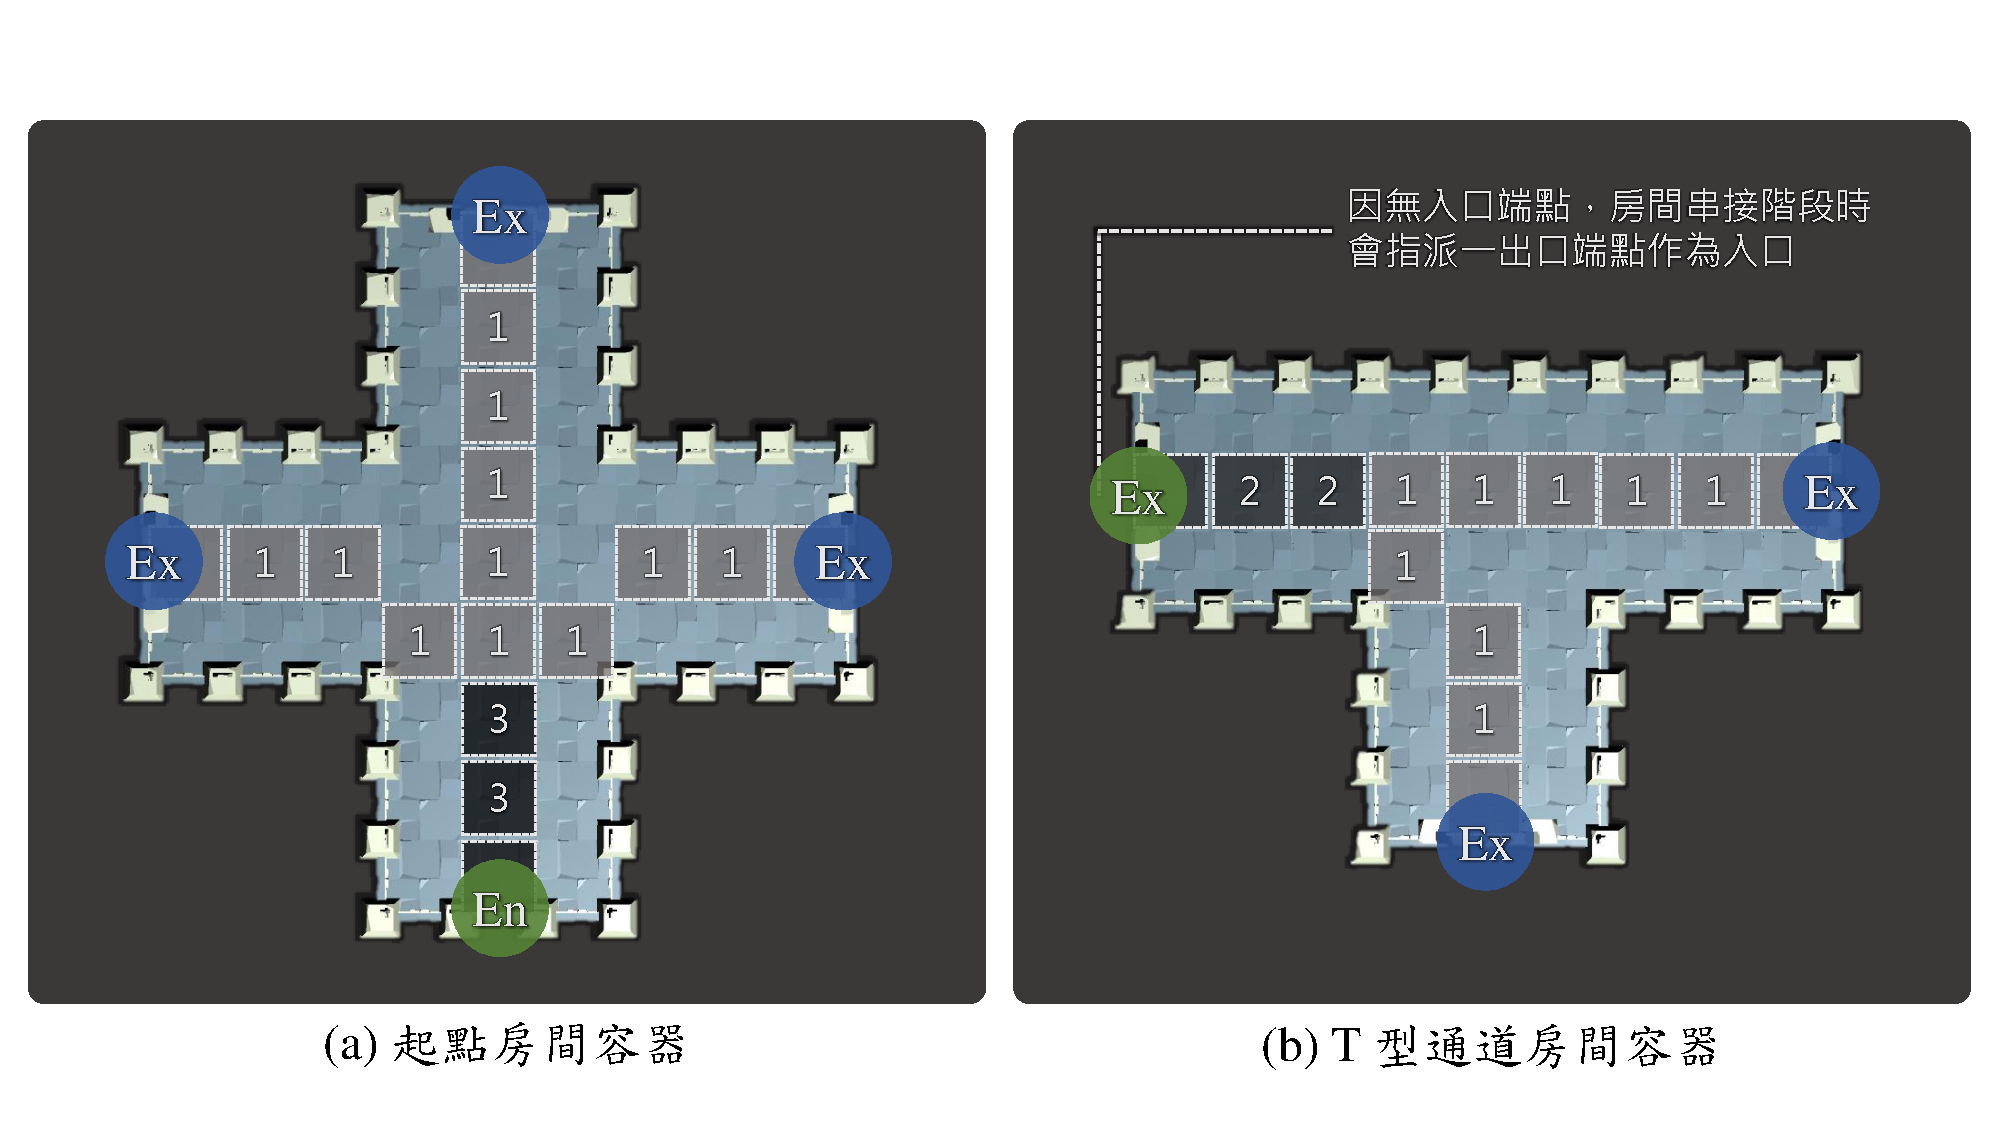
\includegraphics[width=1.0\textwidth]{figures/fitnesses-mainpath.pdf}
    \caption{動線於房間容器的計算方式,圖中數值為行經次數}
    \label{fig:fitnesses-mainpath}
  \end{center}
\end{figure}

\subsubsection{守衛點 (Guard)}
\label{sssec:method-segments-fitnesses-guard}

方程式~\ref{eq:fitnesses-guard} 為守衛點的適應性函數。為體現出敵人會保衛寶箱 ($Treasure$) 與出口 ($Exit$) 的現象,計算敵人 ($E_{i}$) 與為守護對象的遊戲物件 ($O_{j}$) 之間的距離,倘若距離愈近則帶來的影響力愈大。

\begin{equation}
    \label{eq:fitnesses-guard}
    f_{grd} = \sum_{i=1}^{M} \sum_{j=1}^{N} \frac{1}{dist\big(E_{i}, O_{j}\big)}, O_{j} \in \{ Treasure, Exit \}
\end{equation}

\begin{figure}[!htb]
  \begin{center}
    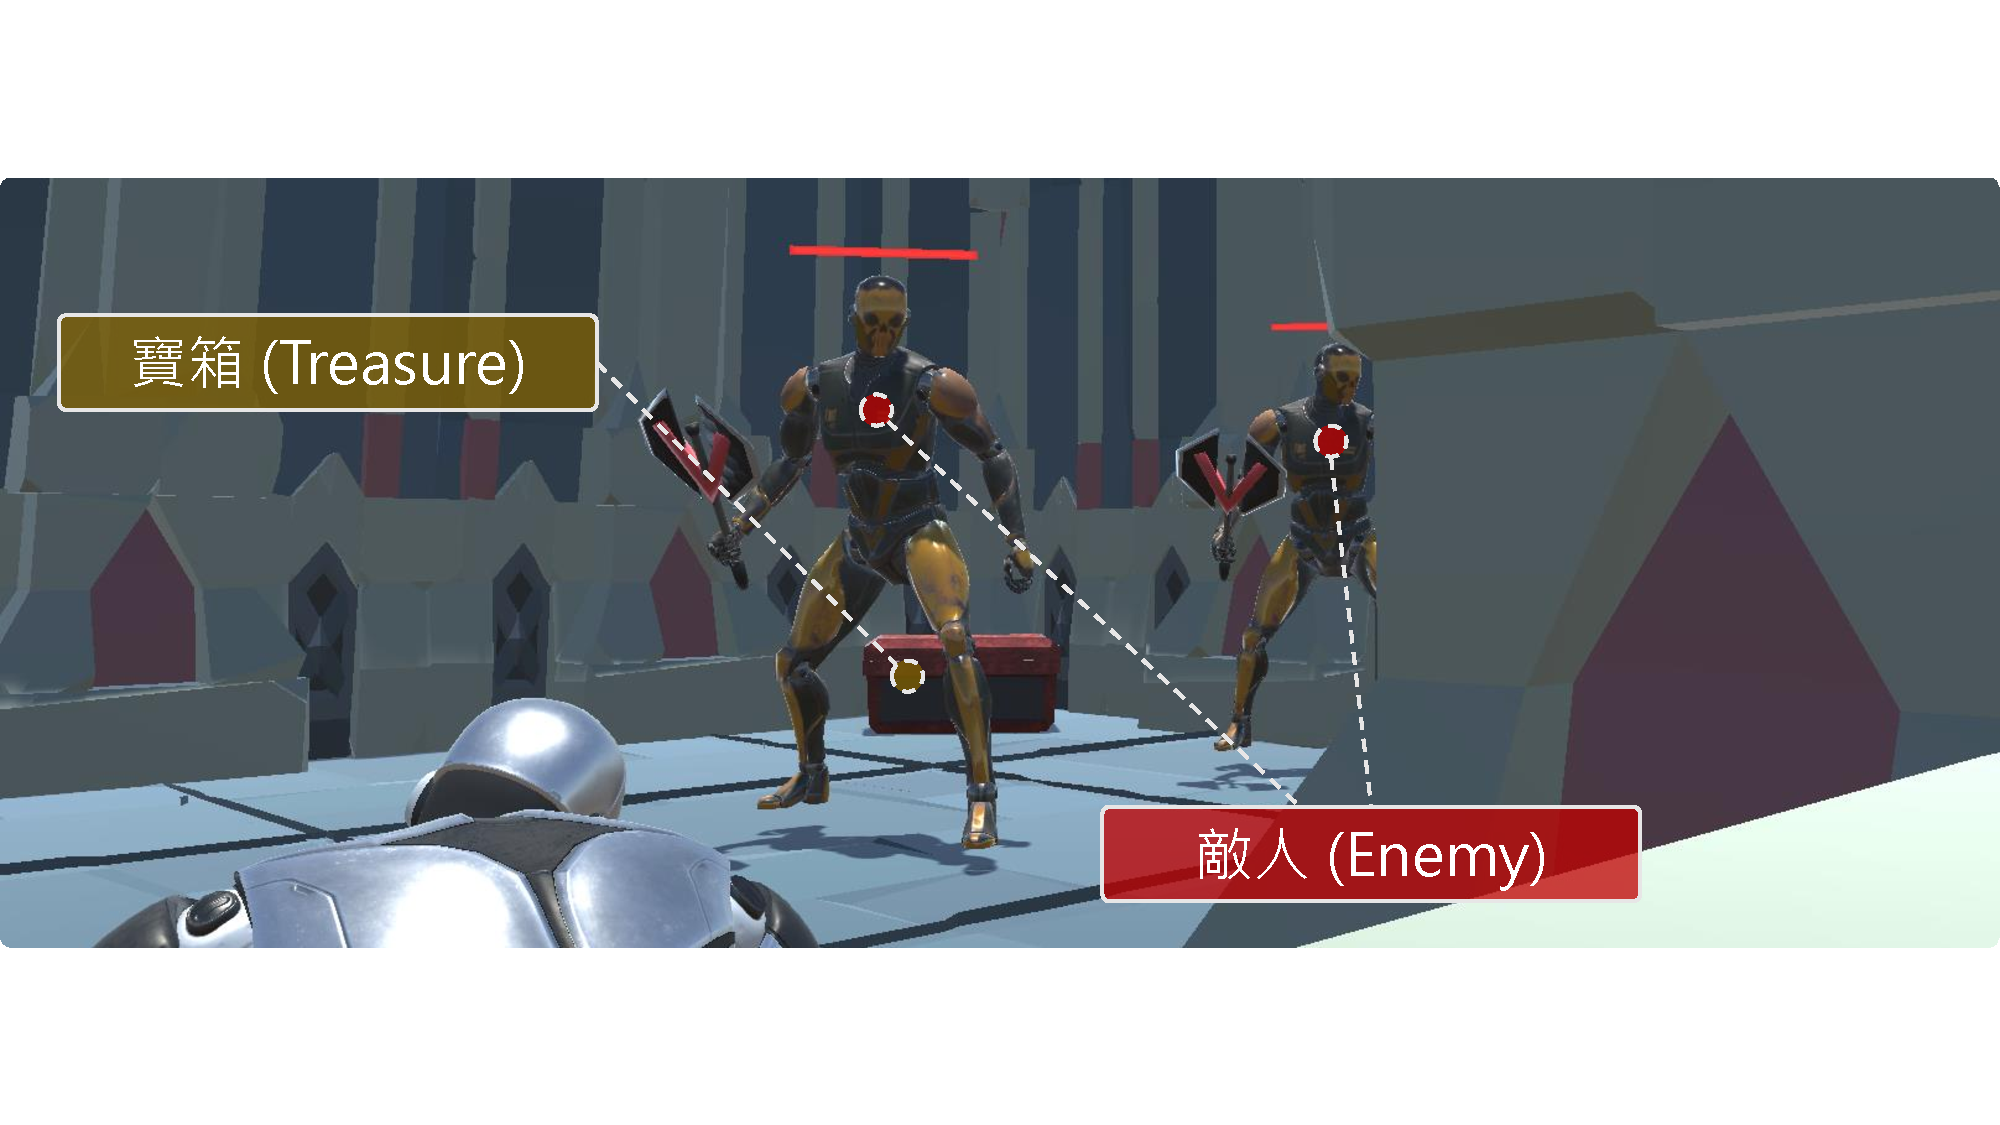
\includegraphics[width=1.0\textwidth]{figures/fitnesses-guard-gameplay.pdf}
    \caption{守衛點指標的遊戲體現情形}
    \label{fig:fitnesses-guard-gameplay}
  \end{center}
\end{figure}

\subsubsection{阻擋點 (Block)}
\label{sssec:method-segments-fitnesses-block}

方程式~\ref{eq:fitnesses-block} 為阻擋點的適應性函數。敵人會專注於阻擋玩家繼續前進,迫使玩家與其發生衝突。$f_{blk}$ 為加總 $M$ 個敵人於空間之動線權重 ($e_{i}$),倘若敵人並未落在動線上,權重則為 $0$。圖~\ref{fig:fitnesses-block-gameplay} 為阻擋點指標的實際遊玩情形,草綠色區塊為系統計算出的空間動線的瓦磚,敵人將會被設置於動線之上阻擋玩家前行。

\begin{equation}
    \label{eq:fitnesses-block}
    f_{blk} = \sum_{i=1}^{M} e_{i}
\end{equation}

\begin{figure}[!htb]
  \begin{center}
    \includegraphics[width=1.0\textwidth]{figures/fitnesses-block-gameplay.pdf}
    \caption{阻擋點指標的遊戲體現情形}
    \label{fig:fitnesses-block-gameplay}
  \end{center}
\end{figure}

\subsubsection{攔截點 (Intercept)}
\label{sssec:method-segments-fitnesses-intercept}

方程式~\ref{eq:fitnesses-intercept} 為攔截點的適應性函數。與阻擋點近似,但敵人會避免被配置在空間動線上,為求快速追擊玩家為目的,將圍繞在空間動線附近。各敵人 ($E_{i}$) 越接近空間動線各點 ($MP_{j}$) 時影響愈大,且動線權重 ($mp_{j}$) 亦會影響加權程度。圖~\ref{fig:fitnesses-intercept-gameplay} 為攔截點指標的實際遊玩情形,草綠色區塊為系統計算出的空間動線的瓦磚,敵人將會被設置於動線周圍快速地攔截玩家。

\begin{equation}
    \label{eq:fitnesses-intercept}
    f_{itc} = \sum_{i=1}^{M} \sum_{j=1}^{N} \Big( \frac{1}{dist(E_{i}, MP_{j})} \times mp_{j} \Big), 
    E_{i} \neq MP_{j}
\end{equation}

\begin{figure}[!htb]
  \begin{center}
    \includegraphics[width=1.0\textwidth]{figures/fitnesses-intercept-gameplay.pdf}
    \caption{攔截點指標的遊戲體現情形}
    \label{fig:fitnesses-intercept-gameplay}
  \end{center}
\end{figure}

\subsubsection{巡邏點 (Patrol)}
\label{sssec:method-segments-fitnesses-patrol}

方程式~\ref{eq:fitnesses-patrol} 為巡邏點的適應性函數。確保敵人擁有足夠的空間能夠進行移動,使其進行巡邏行為。$f_{ptl}$ 為 $M$ 個敵人 ($E_{i}$) 其方圓半徑 ($r$) 內相鄰可行走瓦磚之數量總合,計算各個可行走瓦磚 ($P_{j}$) 與敵人的直線距離,若距離小於或等於 $r$ 則值為 $1$,反之為 $0$。於本次實驗中,將採用 $r=3$ 作為實驗範例,該數值可由遊戲設計師決定。圖~\ref{fig:fitnesses-patrol-gameplay} 為巡邏點指標的實際遊玩情形,水藍色區塊為系統計算出的相鄰可走瓦磚,敵人會在此區域內執行巡邏的。

\begin{equation}
    \label{eq:fitnesses-patrol}
    f_{ptl} = \sum_{i=1}^{M} neighbor(E_i, r)
\end{equation}
\begin{gather*}
    neighbor(Obj, r) = \sum_{j=1}^{N} isNeighbor(Obj, P_{j}, r)
      \begin{cases}
        1, & \mbox{if } dist(Obj, P_{j}) \leq r \\
        0, & \mbox{if } dist(Obj, P_{j}) > r
      \end{cases}
\end{gather*}

\begin{figure}[!htb]
  \begin{center}
    \includegraphics[width=1.0\textwidth]{figures/fitnesses-patrol-gameplay.pdf}
    \caption{巡邏點指標的遊戲體現情形}
    \label{fig:fitnesses-patrol-gameplay}
  \end{center}
\end{figure}

% \subsubsection{支援點 (Support)}
% \label{sssec:method-segments-fitnesses-support}

% 敵人 ($E_{i}$, $E_{j}$) 之間擁有一定程度的護援關係,當敵人彼此的距離愈低其影響程度越大,同時該敵人 ($E_{i}$) 必須遠離動線 ($MP_{k}$)。

% \begin{equation}
% f_{sup}=\frac{1}{N} \sum_{i=1}^{N} \bigg( \frac{1}{N} \sum_{\substack{j=1 \\ j \neq i}}^{N} \frac{1}{dist(E_{i}, E_{j})} + \frac{1}{M} \sum_{k=1}^{M} \frac{1}{dist(E_{i}, MP_{k})} \bigg)
% \end{equation}

% \begin{figure}[!htb]
%   \begin{center}
%     \includegraphics[width=1.0\textwidth]{figures/under_construction.png}
%     \caption{支援點指標的遊戲體現情形}
%     \label{fig:fitnesses-support-gameplay}
%   \end{center}
% \end{figure}

% \subsubsection{陷阱點 (Trapped)}
% \label{sssec:method-segments-fitnesses-trapped}

% \begin{equation}
%     f_{trp} = 
% \end{equation}

% \subsubsection{死角點 (Neglected)}
% \label{sssec:method-segments-fitnesses-neglected}

% 由於房與房之間的牆壁阻隔,使得敵人能夠埋伏於入口附近之死角處,出奇不意地對玩家展開攻擊。為了體現出這種現象,我們將敵人 ($E_{i}$) 與空間動線上各點 ($MP_{i}$),兩端點連線之對角線所構成的立方體,立方體所涵蓋各座標點 ($N_{j}$) 至該對角線的距離為 $d_{k}$,隨著距離增加影響程度會衰減;$vis_{k}$ 為該點的可視情形,若有不可視的座標存在便會提高適應值。隨著動線的順序演進,影響程度逐漸衰減。

% \begin{equation}
%     Under construction
% \end{equation}


% \subsubsection{至高點 (Dominated)}
% \label{sssec:method-segments-fitnesses-dominated}

% 當玩家可能所在動線上之位置 ($MP_{j}$) 與敵人的位置 ($E_{i}$) 具有高低差時,敵人便適合採取遠程攻擊;為了提供玩家思考對付遠程敵人的緩衝時間,將敵人配置於動線末端附近是較好的選擇,$j$ 隨著動線的順序演進,影響程度逐漸增幅。

% \begin{equation}
% f_{dom}=\sum_{i=1}^{N} \sum_{j=1}^{M} \Big( \frac{1}{dist\big(E_{i}, MP_{j}\big)} \times mp_{j} \times j \times high(E_{i}, MP_{j}) \Big)
% \end{equation}


\subsection{制衡取向的適應性函數}
\label{ssec:method-segments-balancefitness}

於~\ref{ssec:method-segments-fitnesses} 小節所提及的適應性函數中,函數皆有著一項共通點,便是隨著符合遊玩特徵的物件數量與適應值呈現顯著正相關,隨著演化代數的提升至終導致房間容器充斥著大量的遊戲物件。然而這樣的遊玩體驗在絕大多數都是不可行的,因此需要針對現有適應性函數所衍生出的特性,設計抑制其得分隨著數量級的成長。

方程式~\ref{eq:fitnesses-density} 控制該房間容器出現的遊戲物件總數。房間容器的物件總數上限為 $M$、下限為 $N$,若遊戲物件總數 $O$ 於數量範圍內可得 $1$ 分,反之得 $0$ 分,本適應性函數的權重固定為其餘權重絕對值之合,最小為 $1$, $w_{dst} = max(1, \sum_{i=1}^{amount} \lvert w_{i}\rvert)$。

\begin{equation}
    \label{eq:fitnesses-density}
    f_{dst} = \begin{cases}
                  1, & \mbox{if } N \leq O \leq M \\
                  0, & \mbox{if } O<N \text{ or } O>M
              \end{cases}
\end{equation}

% \subsection{負數權重的適應性函數}
% \label{ssec:method-segments-minusscores}

% 在~\ref{sssec:method-segments-fitnesses-guard} 守衛點指標的設計中,當權重為正數時能夠體現出「需要被保護的物件,其周圍分配敵方單位進行守衛」的遊玩特徵,且在多個物件的情形下儘可能平均分配敵方單位;反之,負數權重便會體現出「數量愈不平均的守衛情形」。緣故為設計守衛點指標時,並無針對寶箱的數量進行控管而導致。

\subsection{多項適應性函數合併}
\label{ssec:method-segments-multiobjectives}

在設計適應性函數初期,為求多個適應性函數相互牽制,進而求得限制條件的最佳解。而初期函數會力求場上所有的敵人必須盡可能符合各項指標,舉例來說,在某一房間容器的設定中,我們將守衛點、阻擋點的權重調整至 $1$,其餘指標將不採計得分即不調整權重,倘若場面上存在著敵人 A 與 敵人 B,他們會同時被設置在動線上且一定距離內會有作為守護對象的寶箱物件。但對於遊戲設計師在某些情形下,敵人 A 與敵人 B 僅需要分別符合守衛點、阻擋點指標,才是理想中的遊玩特徵。因此,我們定義「首次出現相關遊玩特徵的得分幅度最顯著」,並依照出現數量逐漸下降成長幅度且逼近於 $1$,呈現近似於對數函數圖形的曲線,因此上述兩種情形都有機會成為演化過程中的最適解。取代原先的線性成長關係,進行數值的標準化,強制將值域規範至 $[0, 1]$ 以求最後適應性函數加權總分時,不偏袒任何適應性函數以達到公平基準,並於第~\ref{sec:experiment-normalized} 節進行相關驗證。

方程式~\ref{eq:fitnesses-all} 中定義房間容器(個體)的品質,採計共 $M$ 種適應性函數,第 $i$ 項適應值為 $f_{i}$ 並經過標準化 $Normalized(f_{i}) = [0, 1]$,依照各函數得分與其權重值 $w_{i} = [-1, 1]$ 加權後加總得到 $f_{all}$。而標準化由個體分數 $f_{i}$ 除以該世代最高得分 $f_{i}\cdot max$ 開 $c$ 次方根。

\begin{equation}
    \label{eq:fitnesses-all}
    f_{all} = \sum_{i=1}^{M} (Normalized(f_{i}) \times w_{i})
\end{equation}
\begin{gather*}
    Normalized(f_{i}) = (\frac{f_{i}}{f_{i}\cdot max})^{\frac{1}{c}}
\end{gather*}

圖~\ref{fig:fitnesses-normalized} 中顯示了方程式~\ref{eq:fitnesses-all} 依照不同的非零自然數常數 $c$ 進行適應值的標準化,在此圖中定義 $x\cdot max = 10$ 方便後續的解釋工作。$y_{1}$ 為原始分數除以原始分數最大值之標準化,初期的成長幅度為 $x_{12} - x_{11} = 0.1000$,隨著原始分數的增加並不影響後續的成長幅度 $x_{14} - x_{13} = 0.1000$。為了要體現出前述之定義「首次出現相關遊玩特徵的得分幅度最顯著」的現象,我們對 $y_{1}$ 的數值再進行開 $c$ 次方根,分別以 $c = 2$、$c = 3$ 與 $c = 4$ 得到 $y_{2}$、$y_{3}$ 與 $y_{4}$ 三種線性方程式,其中 $y_{2}$ 的初期成長幅度為 $x_{22} - x_{21} = 0.1310$ 高於 $y_{1}$ 同期的成長幅度,到了後期的成長幅度為 $x_{24} - x_{23} = 0.0847$,逐漸衰減同時已低於 $y_{1}$ 同期的成長幅度,然而這樣的現象隨著常數 $c$ 上升對於分數初期的成長幅度愈大、後期的成長幅度愈小。

\begin{figure}[!htb]
  \begin{center}
    \includegraphics[width=1.0\textwidth]{figures/fitnesses-normalized.pdf}
    \caption{適應值進行標準化}
    \label{fig:fitnesses-normalized}
  \end{center}
\end{figure}

\subsection{套用物件演化機制的房間容器}
\label{ssec:method-segments-appliedonvolumes}

綜合上述小節,不同房間容器類型會有對應的戰略配置。~\ref{ssec:method-spacepieces-types} 小節所介紹的房間容器外,在本小節追加了戰鬥通道的房間容器,與前章節提及之通道不同處,在戰鬥通道中玩家恐會遭遇敵方單位。戰鬥通道的格局是經過特殊設計的,敵方單位能夠依照不同房型格局進行對應的戰鬥策略,見圖~\ref{fig:roomtype-mainpath-extend}。因此依照房間容器類型設置不同的適應性函數權重,逐一定義各自的適應性函數權重值。

\begin{figure}[!htb]
  \begin{center}
    \includegraphics[width=1.0\textwidth]{figures/roomtype-mainpath-extend.pdf}
    \caption{擴充房間容器,戰鬥通道的房間容器結構}
    \label{fig:roomtype-mainpath-extend}
  \end{center}
\end{figure}

\subsubsection{寶藏房}
\label{sssec:method-segments-appliedonvolumes-treasure}

寶藏房的端點識別物僅只有一個入口端點,便不存在空間動線,與空間動線相關的適應性函數不予採計。圖~\ref{fig:applied-ga-on-volume-treasure} 是寶藏房的演化結果。

\begin{itemize}
  \setlength\itemsep{-0.5em}
  \item 守衛點權重: $1.00$
  \item 遊戲物件數量限制: $[3, 5]$
\end{itemize}

\begin{figure}[H]
  \begin{center}
    \includegraphics[width=1.0\textwidth]{figures/applied-ga-on-volume-treasure.pdf}
    \caption{寶藏房的遊戲物件佈局演化示意} 
    \label{fig:applied-ga-on-volume-treasure}
  \end{center}
\end{figure}

\subsubsection{戰鬥通道(狹路驅逐)}
\label{sssec:method-segments-appliedonvolumes-battlepath-narrow}

戰鬥通道(狹路驅逐)無入口端點、有四個出口端點。在此房間容器中,西方出口為一廣場;東方出口位於二樓;在北方出口與南方出口之間有一狹長的通道,是連接各個出口的必經道路。

在此房間容器的佈局預期讓玩家體驗到重要幹道被敵人所盤據,玩家必須在該幹道上與敵人發生衝突方可通過,便將阻擋點指標之權重設為 $1.00$。圖~\ref{fig:applied-ga-on-volume-battlepath-narrow-i} 是戰鬥通道(狹路驅逐)的演化結果,並以南方出口作為入口。

\begin{itemize}
  \setlength\itemsep{-0.5em}
  \item 阻擋點權重: $1.00$
  \item 遊戲物件數量限制: $[4, 5]$
\end{itemize}

\begin{figure}[H]
  \begin{center}
    \includegraphics[width=1.0\textwidth]{figures/under_construction.png}
    \caption{狹路驅逐情境 I 的遊戲物件佈局演化示意} 
    \label{fig:applied-ga-on-volume-battlepath-narrow-i}
  \end{center}
\end{figure}

基於上述情境,在西方廣場或其它寬廣地區,亦有機會設置敵人進行巡邏監視,便將巡邏點指標之權重設為 $0.75$。圖~\ref{fig:applied-ga-on-volume-battlepath-narrow-ii} 是戰鬥通道(狹路驅逐)的演化結果,並以南方出口作為入口。

\begin{itemize}
  \setlength\itemsep{-0.5em}
  \item 阻擋點權重: $1.00$
  \item 巡邏點權重: $0.75$
  \item 遊戲物件數量限制: $[4, 5]$
\end{itemize}

\begin{figure}[H]
  \begin{center}
    \includegraphics[width=1.0\textwidth]{figures/under_construction.png}
    \caption{狹路驅逐情境 II 的遊戲物件佈局演化示意} 
    \label{fig:applied-ga-on-volume-battlepath-narrow-ii}
  \end{center}
\end{figure}

\subsubsection{戰鬥通道(鎮守要道)}
\label{sssec:method-segments-appliedonvolumes-battlepath-trunk}

戰鬥通道(鎮守要道)有一個入口端點及一個出口端點,在此房間容器的佈局與狹路驅逐近似,但敵人將專注於戰鬥陣行,將不會存在寶箱。圖~\ref{fig:applied-ga-on-volume-battlepath-trunk} 是戰鬥通道(鎮守要道)的演化結果。

\begin{itemize}
  \setlength\itemsep{-0.5em}
  \item 阻擋點權重: $1.00$
  % \item 支援點權重: $0.75$
  \item 巡邏點權重: $0.50$
  \item 守衛點權重: $-1.00$
  \item 遊戲物件數量限制: $[3, 5]$
\end{itemize}

\begin{figure}[H]
  \begin{center}
    \includegraphics[width=1.0\textwidth]{figures/applied-ga-on-volume-battlepath-trunk.pdf}
    \caption{鎮守要道情境的遊戲物件佈局演化示意} 
    \label{fig:applied-ga-on-volume-battlepath-trunk}
  \end{center}
\end{figure}

\subsubsection{其餘房間容器}
\label{sssec:method-segments-appliedonvolumes-others}

其餘未被定義的房型,像是入口、出口、一般通道 ... 等,因設計需求將不配置任何遊戲物件,即不參與相關的演化流程。

\begin{figure}[!htb]
  \begin{center}
    \includegraphics[width=1.0\textwidth]{figures/under_construction.png}
    \caption{將關卡中全部房間容器進行遊戲物件的佈局演化} 
    \label{fig:applied-ga-on-volume-all}
  \end{center}
\end{figure}

\section{方法彙整與總結}
\label{sec:method-summary}

第~\ref{sec:method-missiongrammars} 小節介紹了任務語法,讓關卡設計師能透過抽象宏觀的概念,藉由直覺的圖形介面生成出任務圖,表達出遊玩流程的拓撲結構。第~\ref{sec:method-spacepieces} 小節介紹了空間建構,從建構房間容器的最小體素單位至端點識別物,並且透過改寫將任務圖轉換至遊戲空間。第 ~\ref{sec:method-segments} 小節介紹了地圖片段演化的方法,將房間容器依照不同的戰略要素,給予不同遊玩特徵指標的權重,最後利用基因演算法逐步得到遊戲物件的關卡佈局。
	% Quickly landscape for experiment page.
\newcommand{\landscapeexperimentpage}[1]{{
\begin{landscape}
  \begin{minipage}[t]{0.97\linewidth}
    \raggedleft
    \begin{minipage}[t]{0.97\linewidth}
      \centering
      #1
    \end{minipage}
  \end{minipage}
\end{landscape}
}}

% Quickly create the table.
\newcommand{\gasettingstable}[4]{{
\begin{table}[H]
  \centering
  \caption{實驗 #2 之基因演算法參數配置}
  \label{tbl:settings-of-experiment-#1}
  \bigskip
  \vspace{-5mm}
  \begin{minipage}[t]{0.35\linewidth}
    \centering
    \begin{tabular}[t]{| c | c | c |}
      \hline
      \multicolumn{1}{ |c| }{回合次數}
        & \multicolumn{1}{ c| }{世代數量}
        & \multicolumn{1}{ c| }{個體數量} \\\hline
      #3
      \hline
    \end{tabular}
  \end{minipage}
  \begin{minipage}[t]{0.35\linewidth}
    \centering
    \begin{tabular}[t]{| c | c | c |}
      \hline
      \multicolumn{1}{ |c| }{指標}
        & \multicolumn{1}{ c| }{權重}
        & \multicolumn{1}{ c| }{備注} \\\hline
      #4
      \hline
    \end{tabular}
  \end{minipage}
\end{table}
}}

% Quickly show the evolution results via figure.
\newcommand{\galayoutresults}[2]{{
\includegraphics[width=0.90\linewidth]{figures/experiments/#1-results.pdf}
\captionof{figure}{實驗 #2 的演化結果及各演化耗時}
\label{fig:experiment-#1-results}
}}

% Quickly create the table.
\newcommand{\garesultssubtable}[1]{{
\begin{minipage}[t]{0.48\linewidth}
  \begin{tabular}[t]{
    | >{\centering\arraybackslash}m{0.8cm}
    | >{\centering\arraybackslash}m{1.7cm}
    | >{\centering\arraybackslash}m{1.5cm} 
    | >{\centering\arraybackslash}m{1.0cm} | }
    \hline
    \multirow{2}{*}{回合} & 指標 & \multicolumn{1}{ c| }{適應值} & \multicolumn{1}{ c| }{權重} \\\cline{2-4}
    & \multicolumn{3}{ c| }{總適應值} \\\hline
    #1
  \end{tabular}
\end{minipage}
}}

\newcommand{\garesultstable}[5]{{
\begin{table}[H]
  \centering
  \caption{實驗 #2 - 共 #3 回合的最佳個體之標準化加權適應值}
  \label{tbl:result-of-experiment-#1}
  \bigskip
  \vspace{-5mm}
  \garesultssubtable{#4}
  \garesultssubtable{#5}
\end{table}
}}

\chapter{實驗結果與分析}
\label{cha:experiment}

本章節將探討前述章節之方法是否符合研究目標,將進行以下實驗:第~\ref{sec:experiment-results} 小節中,針對所挑選的房間採用不同權重的適應性函數,其演化的世代數量、群族的個體數量會如何影響房間內的遊戲物件之配置結果。

\section{實驗定義}
\label{sec:experiment-definition}

我們使用 Invector 公司開發的 \textit{Third Person Controller - Melee Combat Template} 套件(以下簡稱 \textit{3rdPC})進行遊戲物件的設置。\textit{3rdPC} 提供遊戲開發者快速建構玩家控制角色 (Player Character) 、非玩家控制角色 (Non-Player Character) 與其角色控制器或人工智能,並可製作任何類型的第三人稱動作冒險遊戲或角色扮演遊戲。第~\ref{ssec:experiment-gameplaymanual} 小節中,說明 \textit{3rdPC} 提供的玩家角色的操作使用說明;第~\ref{ssec:experiment-gameobjects} 小節中,解釋實驗中的採用遊戲物件,其象徵意義與玩家角色互動方式;第~\ref{ssec:experiment-parameters} 小節中,將定義屬實驗變因的相關參數設定,包含任務語法與基因演算法。

\subsection{遊戲操作說明}
\label{ssec:experiment-gameplaymanual}

玩家所控制的角色能夠移動、攻擊、防禦、跳躍與蹲下等動作。移動使用方向鍵,角色朝前後左右與其斜向組合鍵的方向移動,過程中按下 shift 按鍵將會切換至奔跑模式;攻擊使用滑鼠左鍵單擊,連續使用能夠進行三階段的攻擊,每次攻擊將消耗耐力值;防禦使用滑鼠右鍵單擊,能夠減少受到敵方攻擊的損傷;跳躍按鍵鍵盤 space 按鍵,角色能夠進行原地跳躍,在移動或奔跑的過程中亦可使用;蹲下按下鍵盤 c 按鍵,角色能夠緩慢的移動,適合觀察敵方戰況的同時進行移動。

\subsection{遊戲物件說明}
\label{ssec:experiment-gameobjects}

敵人會在玩家靠近,且進入攻擊視野範圍時,追擊玩家。當玩家靠近並朝向寶箱時,按下鍵盤 E 按鍵便可以開啟寶箱,取得寶箱內容物。當玩家碰觸到陷阱時,會受到一定程度的損傷。

% \subsubsection{敵人}
% \label{sssec:experiment-gameobjects-enemy}

% 敵人 (編輯中)。

% \subsubsection{寶箱}
% \label{sssec:experiment-gameobjects-treasure}

% 當玩家靠近並朝向寶箱時,按下鍵盤 E 按鍵便可以開啟寶箱,取得寶箱內容物。

% \subsubsection{陷阱}
% \label{sssec:experiment-gameobjects-trap}

% 當玩家碰觸到陷阱時,會受到一定程度的損傷。

\subsection{實驗參數設定}
\label{ssec:experiment-parameters}

% 在任務語法階段時,我們將非合法 ... (編輯中)

房間容器的遊戲物件佈局演化階段時,每一次世代的演化過程有 $80\%$ 機率於父母代進行兩點交配 (two-point crossover);$10\%$ 機率令衍生子代會進行突變,個體的染色體有 $5\%$ 至 $20\%$ 的基因會轉換成其它的遊戲物件種類。

然而各個房間容器的適應性函數之權重如何決定?將取決於關卡設計師對於該房間容器預期產出進行調整,若希望該指標能越出現於房間容器,則將其權重調高;反之,越不希望該指標出現在房間容器,則將其權重調低;若不理會該指標的體現與否,則將其權重設定為 $0$。在本次研究的系列實驗中,將以關卡設計師視角進行權重的指派,並不代表實驗中所使用的權重最能夠體現其房間容器。

\section{資料收集}
\label{sec:experiment-datacollection}

在資料收集階段中,將收集第~\ref{sec:method-segments} 節中,房間容器進行基因演算法演化時,於實驗過程中輸出 CSV 格式資料。表~\ref{tbl:structure-of-rawdata-scores} 紀錄各回合、世代中,其各個個體(單一染色體)的適應值的得分狀況;表~\ref{tbl:structure-of-rawdata-positions} 紀錄各回合、世代中,其各個個體(單一染色體)的所有座標資訊與其遊戲物件類型。更多的原始資料節錄內容可參見附錄資源。

\begin{table}[!htb]
  \centering
  \caption{演化適應值資料節錄}
  \label{tbl:structure-of-rawdata-scores}
  \bigskip
  \begin{tabular}{| c | c | c | l | l |}
    \hline
    \multicolumn{1}{ |c| }{回合編號}
      & \multicolumn{1}{ c| }{世代編號}
      & \multicolumn{1}{ c| }{染色體編號}
      & \multicolumn{1}{ c| }{指標}
      & \multicolumn{1}{ c| }{得分} \\\hline
    1 & 1 & 1 & Block     & 0 \\
    1 & 1 & 1 & Intercept & 0 \\
    1 & 1 & 1 & Patrol    & 0 \\
    1 & 1 & 1 & Guard     & 0 \\
    1 & 1 & 1 & Support   & 0 \\
    1 & 1 & 1 & Block     & 0 \\
    1 & 1 & 1 & Intercept & 0 \\
    \hline
  \end{tabular}
\end{table}

\begin{table}[!htb]
  \centering
  \caption{演化座標資料節錄}
  \label{tbl:structure-of-rawdata-positions}
  \bigskip
  \begin{tabular}{| c | c | c | l | c |}
    \hline
    \multicolumn{1}{ |c| }{回合編號}
      & \multicolumn{1}{ c| }{世代編號}
      & \multicolumn{1}{ c| }{染色體編號}
      & \multicolumn{1}{ c| }{座標}
      & \multicolumn{1}{ c| }{遊戲物件類型} \\\hline
    1 & 1 & 1 & (1.0, 1.0, 0.0) & Empty \\
    1 & 1 & 1 & (0.0, 1.0, 0.0) & Empty \\
    1 & 1 & 1 & (0.0, 1.0, 1.0) & Empty \\
    1 & 1 & 1 & (0.0, 1.0, 2.0) & Empty \\
    1 & 1 & 1 & (0.0, 1.0, 3.0) & Empty \\
    \hline
  \end{tabular}
\end{table}

\section{演化結果與其品質}
\label{sec:experiment-results}

在第~\ref{ssec:method-segments-appliedonvolumes} 小節中,展示了寶藏房與戰鬥通道(狹路驅逐、鎮守要道)三種空間的局部佈局演化結果,隨著房間容器搭配不同的適應性函數,便能夠生成出多樣性的遊戲物件佈局。在本小節的各實驗中,將針對上述三種房間容器的演化結果做更進一步的分析,紀錄佈局演化結果上視圖與最佳個體之標準化加權適應值,由於各實驗、各回合產生的區域極值不同,影響標準化的量尺不同,我們便分開探討各實驗中的適應值成長趨勢。

\landscapeexperimentpage{
  \subsection{寶藏房}
  \label{ssec:experiment-results-treasure}

  \subsubsection{實驗 A - 世代數量的影響}
  \label{sssec:experiment-results-treasure-gen}

  \gasettingstable{a1}{A1}
    { $10$ & $50$ & $100$ \\ }
    {
      守衛點       & $1.00$ & \\
      遊戲物件數量 & $1.00$ & $Limit: [2, 5]$ \\
    }

  \galayoutresults{a1}{A1}
}

\garesultstable{a1}{A1}{10}
  {
    \multirow{3}{*}{$1$}  & 守衛點   & $0.7002$ & $1$ \\\cline{2-4}
                          & 物件數量 & $1.0000$ & $1$ \\\cline{2-4}
                          & \multicolumn{3}{ r| }{$1.7002$} \\\hline
    \multirow{3}{*}{$2$}  & 守衛點   & $0.6661$ & $1$ \\\cline{2-4}
                          & 物件數量 & $1.0000$ & $1$ \\\cline{2-4}
                          & \multicolumn{3}{ r| }{$1.6661$} \\\hline
    \multirow{3}{*}{$3$}  & 守衛點   & $0.7953$ & $1$ \\\cline{2-4}
                          & 物件數量 & $1.0000$ & $1$ \\\cline{2-4}
                          & \multicolumn{3}{ r| }{$1.7953$} \\\hline
    \multirow{3}{*}{$4$}  & 守衛點   & $0.5995$ & $1$ \\\cline{2-4}
                          & 物件數量 & $1.0000$ & $1$ \\\cline{2-4}
                          & \multicolumn{3}{ r| }{$1.5995$} \\\hline
    \multirow{3}{*}{$5$}  & 守衛點   & $0.7903$ & $1$ \\\cline{2-4}
                          & 物件數量 & $1.0000$ & $1$ \\\cline{2-4}
                          & \multicolumn{3}{ r| }{$1.7903$} \\\hline
  }
  {
    \multirow{3}{*}{$6$}  & 守衛點   & $0.7415$ & $1$ \\\cline{2-4}
                          & 物件數量 & $1.0000$ & $1$ \\\cline{2-4}
                          & \multicolumn{3}{ r| }{$1.7415$} \\\hline
    \multirow{3}{*}{$7$}  & 守衛點   & $0.6859$ & $1$ \\\cline{2-4}
                          & 物件數量 & $1.0000$ & $1$ \\\cline{2-4}
                          & \multicolumn{3}{ r| }{$1.6859$} \\\hline
    \multirow{3}{*}{$8$}  & 守衛點   & $0.6357$ & $1$ \\\cline{2-4}
                          & 物件數量 & $1.0000$ & $1$ \\\cline{2-4}
                          & \multicolumn{3}{ r| }{$1.6357$} \\\hline
    \multirow{3}{*}{$9$}  & 守衛點   & $0.6792$ & $1$ \\\cline{2-4}
                          & 物件數量 & $1.0000$ & $1$ \\\cline{2-4}
                          & \multicolumn{3}{ r| }{$1.6792$} \\\hline
    \multirow{3}{*}{$10$} & 守衛點   & $0.6840$ & $1$ \\\cline{2-4}
                          & 物件數量 & $1.0000$ & $1$ \\\cline{2-4}
                          & \multicolumn{3}{ r| }{$1.6840$} \\\hline
  }


\landscapeexperimentpage{
  \gasettingstable{a2}{A2}
    { $10$ & $100$ & $100$ \\ }
    {
      守衛點       & $1.00$ & \\
      遊戲物件數量 & $1.00$ & $Limit: [2, 5]$ \\
    }

  \galayoutresults{a2}{A2}
}

\garesultstable{a2}{A2}{10}
  {
    \multirow{3}{*}{$1$}  & 守衛點   & $0.7416$ & $1$ \\\cline{2-4}
                          & 物件數量 & $1.0000$ & $1$ \\\cline{2-4}
                          & \multicolumn{3}{ r| }{$1.7416$} \\\hline
    \multirow{3}{*}{$2$}  & 守衛點   & $0.6654$ & $1$ \\\cline{2-4}
                          & 物件數量 & $1.0000$ & $1$ \\\cline{2-4}
                          & \multicolumn{3}{ r| }{$1.6654$} \\\hline
    \multirow{3}{*}{$3$}  & 守衛點   & $0.6333$ & $1$ \\\cline{2-4}
                          & 物件數量 & $1.0000$ & $1$ \\\cline{2-4}
                          & \multicolumn{3}{ r| }{$1.6333$} \\\hline
    \multirow{3}{*}{$4$}  & 守衛點   & $0.7108$ & $1$ \\\cline{2-4}
                          & 物件數量 & $1.0000$ & $1$ \\\cline{2-4}
                          & \multicolumn{3}{ r| }{$1.7108$} \\\hline
    \multirow{3}{*}{$5$}  & 守衛點   & $0.7356$ & $1$ \\\cline{2-4}
                          & 物件數量 & $1.0000$ & $1$ \\\cline{2-4}
                          & \multicolumn{3}{ r| }{$1.7356$} \\\hline
  }
  {
    \multirow{3}{*}{$6$}  & 守衛點   & $0.6697$ & $1$ \\\cline{2-4}
                          & 物件數量 & $1.0000$ & $1$ \\\cline{2-4}
                          & \multicolumn{3}{ r| }{$1.6697$} \\\hline
    \multirow{3}{*}{$7$}  & 守衛點   & $0.7244$ & $1$ \\\cline{2-4}
                          & 物件數量 & $1.0000$ & $1$ \\\cline{2-4}
                          & \multicolumn{3}{ r| }{$1.7244$} \\\hline
    \multirow{3}{*}{$8$}  & 守衛點   & $0.8320$ & $1$ \\\cline{2-4}
                          & 物件數量 & $1.0000$ & $1$ \\\cline{2-4}
                          & \multicolumn{3}{ r| }{$1.8320$} \\\hline
    \multirow{3}{*}{$9$}  & 守衛點   & $0.7317$ & $1$ \\\cline{2-4}
                          & 物件數量 & $1.0000$ & $1$ \\\cline{2-4}
                          & \multicolumn{3}{ r| }{$1.7317$} \\\hline
    \multirow{3}{*}{$10$} & 守衛點   & $0.6270$ & $1$ \\\cline{2-4}
                          & 物件數量 & $1.0000$ & $1$ \\\cline{2-4}
                          & \multicolumn{3}{ r| }{$1.6270$} \\\hline
  }


\landscapeexperimentpage{
  \gasettingstable{a3}{A3}
    { $10$ & $200$ & $100$ \\ }
    {
      守衛點       & $1.00$ & \\
      遊戲物件數量 & $1.00$ & $Limit: [2, 5]$ \\
    }

  \galayoutresults{a3}{A3}
}

\garesultstable{a3}{A3}{10}
  {
    \multirow{3}{*}{$1$}  & 守衛點   & $0.8235$ & $1$ \\\cline{2-4}
                          & 物件數量 & $1.0000$ & $1$ \\\cline{2-4}
                          & \multicolumn{3}{ r| }{$1.8235$} \\\hline
    \multirow{3}{*}{$2$}  & 守衛點   & $0.6567$ & $1$ \\\cline{2-4}
                          & 物件數量 & $1.0000$ & $1$ \\\cline{2-4}
                          & \multicolumn{3}{ r| }{$1.6567$} \\\hline
    \multirow{3}{*}{$3$}  & 守衛點   & $0.6528$ & $1$ \\\cline{2-4}
                          & 物件數量 & $1.0000$ & $1$ \\\cline{2-4}
                          & \multicolumn{3}{ r| }{$1.6528$} \\\hline
    \multirow{3}{*}{$4$}  & 守衛點   & $0.6531$ & $1$ \\\cline{2-4}
                          & 物件數量 & $1.0000$ & $1$ \\\cline{2-4}
                          & \multicolumn{3}{ r| }{$1.6531$} \\\hline
    \multirow{3}{*}{$5$}  & 守衛點   & $0.6445$ & $1$ \\\cline{2-4}
                          & 物件數量 & $1.0000$ & $1$ \\\cline{2-4}
                          & \multicolumn{3}{ r| }{$1.6445$} \\\hline
  }
  {
    \multirow{3}{*}{$6$}  & 守衛點   & $0.8025$ & $1$ \\\cline{2-4}
                          & 物件數量 & $1.0000$ & $1$ \\\cline{2-4}
                          & \multicolumn{3}{ r| }{$1.8025$} \\\hline
    \multirow{3}{*}{$7$}  & 守衛點   & $0.5842$ & $1$ \\\cline{2-4}
                          & 物件數量 & $1.0000$ & $1$ \\\cline{2-4}
                          & \multicolumn{3}{ r| }{$1.5842$} \\\hline
    \multirow{3}{*}{$8$}  & 守衛點   & $0.7224$ & $1$ \\\cline{2-4}
                          & 物件數量 & $1.0000$ & $1$ \\\cline{2-4}
                          & \multicolumn{3}{ r| }{$1.7224$} \\\hline
    \multirow{3}{*}{$9$}  & 守衛點   & $0.8942$ & $1$ \\\cline{2-4}
                          & 物件數量 & $1.0000$ & $1$ \\\cline{2-4}
                          & \multicolumn{3}{ r| }{$1.8942$} \\\hline
    \multirow{3}{*}{$10$} & 守衛點   & $0.7029$ & $1$ \\\cline{2-4}
                          & 物件數量 & $1.0000$ & $1$ \\\cline{2-4}
                          & \multicolumn{3}{ r| }{$1.7029$} \\\hline
  }


\landscapeexperimentpage{
  \subsubsection{實驗 B - 個體數量的影響}
  \label{sssec:experiment-results-treasure-idv}

  \gasettingstable{b1}{B1}
    { $10$ & $100$ & $50$ \\ }
    {
      守衛點       & $1.00$ & \\
      遊戲物件數量 & $1.00$ & $Limit: [2, 5]$ \\
    }

  % \galayoutresults{b1}{B1}
}

\garesultstable{b2}{B2}{10}
  {
  }
  {
  }


\landscapeexperimentpage{
  \gasettingstable{b2}{B2}
    { $10$ & $100$ & $100$ \\ }
    {
      守衛點       & $1.00$ & \\
      遊戲物件數量 & $1.00$ & $Limit: [2, 5]$ \\
    }

  % \galayoutresults{b2}{B2}
}

\garesultstable{b2}{B2}{10}
  {
  }
  {
  }


\landscapeexperimentpage{
  \gasettingstable{b3}{B3}
    { $10$ & $100$ & $200$ \\ }
    {
      守衛點       & $1.00$ & \\
      遊戲物件數量 & $1.00$ & $Limit: [2, 5]$ \\
    }

  % \galayoutresults{b3}{B3}
}

\garesultstable{b3}{B3}{10}
  {
  }
  {
  }


\subsubsection{小結}
\label{sssec:experiment-results-treasure-summary}

實驗小結實驗小結實驗小結實驗小結實驗小結實驗小結實驗小結實驗小結實驗小結實驗小結實驗小結實驗小結實驗小結實驗小結實驗小結實驗小結

\landscapeexperimentpage{
  \subsection{戰鬥通道(狹路驅逐)}
  \label{ssec:experiment-results-narrow}

  \subsubsection{實驗 C - 世代數量的影響}
  \label{sssec:experiment-results-narrow-gen}

  \gasettingstable{c1}{C1}
    { $10$ & $50$ & $100$ \\ }
    {
      阻攔點       & $1.00$ & \\
      攔截點       & $0.75$ & \\
      % 陷阱點       & $0.75$ & \\
      遊戲物件數量 & $1.00$ & $Limit: [2, 3]$ \\
    }

  % \galayoutresults{c1}{C1}
}

\garesultstable{c1}{C1}{10}
  {
  }
  {
  }


\landscapeexperimentpage{
  \gasettingstable{c2}{C2}
    { $10$ & $100$ & $100$ \\ }
    {
      阻攔點       & $1.00$ & \\
      攔截點       & $0.75$ & \\
      % 陷阱點       & $0.75$ & \\
      遊戲物件數量 & $1.00$ & $Limit: [2, 3]$ \\
    }

  % \galayoutresults{c2}{C2}
}

\garesultstable{c2}{C2}{10}
  {
  }
  {
  }


\landscapeexperimentpage{
  \gasettingstable{c3}{C3}
    { $10$ & $200$ & $100$ \\ }
    {
      阻攔點       & $1.00$ & \\
      攔截點       & $0.75$ & \\
      % 陷阱點       & $0.75$ & \\
      遊戲物件數量 & $1.00$ & $Limit: [2, 3]$ \\
    }

  % \galayoutresults{c3}{C3}
}

\garesultstable{c3}{C3}{10}
  {
  }
  {
  }


\landscapeexperimentpage{
  \subsubsection{實驗 D - 個體數量的影響}
  \label{sssec:experiment-results-narrow-idv}

  \gasettingstable{d1}{D1}
    { $10$ & $100$ & $50$ \\ }
    {
      阻攔點       & $1.00$ & \\
      攔截點       & $0.75$ & \\
      % 陷阱點       & $0.75$ & \\
      遊戲物件數量 & $1.00$ & $Limit: [2, 3]$ \\
    }

  % \galayoutresults{d1}{D1}
}

\garesultstable{d1}{D1}{10}
  {
  }
  {
  }


\landscapeexperimentpage{
  \gasettingstable{d2}{D2}
    { $10$ & $100$ & $100$ \\ }
    {
      阻攔點       & $1.00$ & \\
      攔截點       & $0.75$ & \\
      % 陷阱點       & $0.75$ & \\
      遊戲物件數量 & $1.00$ & $Limit: [2, 3]$ \\
    }

  % \galayoutresults{d2}{D2}
}

\garesultstable{d2}{D2}{10}
  {
  }
  {
  }


\landscapeexperimentpage{
  \gasettingstable{d3}{D3}
    { $10$ & $100$ & $200$ \\ }
    {
      阻攔點       & $1.00$ & \\
      攔截點       & $0.75$ & \\
      % 陷阱點       & $0.75$ & \\
      遊戲物件數量 & $1.00$ & $Limit: [2, 3]$ \\
    }

  % \galayoutresults{d3}{D3}
}

\garesultstable{d3}{D3}{10}
  {
  }
  {
  }


\subsubsection{小結}
\label{sssec:experiment-results-narrow-summary}

實驗小結實驗小結實驗小結實驗小結實驗小結實驗小結實驗小結實驗小結實驗小結實驗小結實驗小結實驗小結實驗小結實驗小結實驗小結實驗小結


\landscapeexperimentpage{
  \subsection{戰鬥通道(鎮守要道)}
  \label{ssec:experiment-results-trunk}

  \subsubsection{實驗 E - 個體數量的影響}
  \label{sssec:experiment-results-trunk-gen}

  \gasettingstable{e1}{E1}
    { $1$ & $50$ & $100$ \\ }
    {
      阻攔點       & $1.00$  & \\
      % 支援點       & $0.75$  & \\
      巡邏點       & $0.50$  & \\
      守衛點       & $-1.00$ & \\
      遊戲物件數量 & $1.00$  & $Limit: [3, 5]$ \\
    }

  \galayoutresults{e1}{E1}
}


\garesultstable{e1}{E1}{10}
  {
    \multirow{5}{*}{$1$}  & 阻擋點   & $1.0000$  & $1$   \\\cline{2-4}
                          & 巡邏點   & $0.5000$  & $0.5$ \\\cline{2-4}
                          & 守衛點   & $0.0000$  & $-1$  \\\cline{2-4}
                          & 物件數量 & $2.5000$  & $2.5$ \\\cline{2-4}
                          & \multicolumn{3}{ r| }{$4.0000$} \\\hline
    \multirow{5}{*}{$2$}  & 阻擋點   & $0.7071$  & $1$   \\\cline{2-4}
                          & 巡邏點   & $0.4787$  & $0.5$ \\\cline{2-4}
                          & 守衛點   & $0.0000$  & $-1$  \\\cline{2-4}
                          & 物件數量 & $2.5000$  & $2.5$ \\\cline{2-4}
                          & \multicolumn{3}{ r| }{$3.6858$} \\\hline
    \multirow{5}{*}{$3$}  & 阻擋點   & $0.0000$  & $1$   \\\cline{2-4}
                          & 巡邏點   & $0.4682$  & $0.5$ \\\cline{2-4}
                          & 守衛點   & $-0.2000$ & $-1$  \\\cline{2-4}
                          & 物件數量 & $2.5000$  & $2.5$ \\\cline{2-4}
                          & \multicolumn{3}{ r| }{$2.7681$} \\\hline
    \multirow{5}{*}{$4$}  & 阻擋點   & $1.0000$  & $1$   \\\cline{2-4}
                          & 巡邏點   & $0.5000$  & $0.5$ \\\cline{2-4}
                          & 守衛點   & $0.0000$  & $-1$  \\\cline{2-4}
                          & 物件數量 & $2.5000$  & $2.5$ \\\cline{2-4}
                          & \multicolumn{3}{ r| }{$4.0000$} \\\hline
    \multirow{5}{*}{$5$}  & 阻擋點   & $1.0000$  & $1$   \\\cline{2-4}
                          & 巡邏點   & $0.4871$  & $0.5$ \\\cline{2-4}
                          & 守衛點   & $0.0000$  & $-1$  \\\cline{2-4}
                          & 物件數量 & $2.5000$  & $2.5$ \\\cline{2-4}
                          & \multicolumn{3}{ r| }{$3.9871$} \\\hline
  }
  {
    \multirow{5}{*}{$6$}  & 阻擋點   & $1.0000$ & $1$   \\\cline{2-4}
                          & 巡邏點   & $0.4859$ & $0.5$ \\\cline{2-4}
                          & 守衛點   & $0.0000$ & $-1$  \\\cline{2-4}
                          & 物件數量 & $2.5000$ & $2.5$ \\\cline{2-4}
                          & \multicolumn{3}{ r| }{$3.9859$} \\\hline
    \multirow{5}{*}{$7$}  & 阻擋點   & $0.7071$ & $1$   \\\cline{2-4}
                          & 巡邏點   & $0.5000$ & $0.5$ \\\cline{2-4}
                          & 守衛點   & $0.0000$ & $-1$  \\\cline{2-4}
                          & 物件數量 & $2.5000$ & $2.5$ \\\cline{2-4}
                          & \multicolumn{3}{ r| }{$3.7071$} \\\hline
    \multirow{5}{*}{$8$}  & 阻擋點   & $0.8165$ & $1$   \\\cline{2-4}
                          & 巡邏點   & $0.4296$ & $0.5$ \\\cline{2-4}
                          & 守衛點   & $0.0000$ & $-1$  \\\cline{2-4}
                          & 物件數量 & $2.5000$ & $2.5$ \\\cline{2-4}
                          & \multicolumn{3}{ r| }{$3.7461$} \\\hline
    \multirow{5}{*}{$9$}  & 阻擋點   & $0.5774$ & $1$   \\\cline{2-4}
                          & 巡邏點   & $0.5000$ & $0.5$ \\\cline{2-4}
                          & 守衛點   & $0.0000$ & $-1$  \\\cline{2-4}
                          & 物件數量 & $2.5000$ & $2.5$ \\\cline{2-4}
                          & \multicolumn{3}{ r| }{$3.5774$} \\\hline
    \multirow{5}{*}{$10$} & 阻擋點   & $1.0000$ & $1$   \\\cline{2-4}
                          & 巡邏點   & $0.4838$ & $0.5$ \\\cline{2-4}
                          & 守衛點   & $0.0000$ & $-1$  \\\cline{2-4}
                          & 物件數量 & $2.5000$ & $2.5$ \\\cline{2-4}
                          & \multicolumn{3}{ r| }{$3.9838$} \\\hline
  }


\landscapeexperimentpage{
  \gasettingstable{e2}{E2}
    { $1$ & $100$ & $100$ \\ }
    {
      阻攔點       & $1.00$  & \\
      % 支援點       & $0.75$  & \\
      巡邏點       & $0.50$  & \\
      守衛點       & $-1.00$ & \\
      遊戲物件數量 & $1.00$  & $Limit: [3, 5]$ \\
    }

  \galayoutresults{e2}{E2}
}

\garesultstable{e2}{E2}{10}
  {
    \multirow{5}{*}{$1$}  & 阻擋點   & $1.0000$ & $1$   \\\cline{2-4}
                          & 巡邏點   & $0.4965$ & $0.5$ \\\cline{2-4}
                          & 守衛點   & $0.0000$ & $-1$  \\\cline{2-4}
                          & 物件數量 & $2.5000$ & $2.5$ \\\cline{2-4}
                          & \multicolumn{3}{ r| }{$3.9965$} \\\hline
    \multirow{5}{*}{$2$}  & 阻擋點   & $0.8660$ & $1$   \\\cline{2-4}
                          & 巡邏點   & $0.4567$ & $0.5$ \\\cline{2-4}
                          & 守衛點   & $0.0000$ & $-1$  \\\cline{2-4}
                          & 物件數量 & $2.5000$ & $2.5$ \\\cline{2-4}
                          & \multicolumn{3}{ r| }{$3.8228$} \\\hline
    \multirow{5}{*}{$3$}  & 阻擋點   & $1.0000$ & $1$   \\\cline{2-4}
                          & 巡邏點   & $0.4887$ & $0.5$ \\\cline{2-4}
                          & 守衛點   & $0.0000$ & $-1$  \\\cline{2-4}
                          & 物件數量 & $2.5000$ & $2.5$ \\\cline{2-4}
                          & \multicolumn{3}{ r| }{$3.9887$} \\\hline
    \multirow{5}{*}{$4$}  & 阻擋點   & $0.7071$ & $1$   \\\cline{2-4}
                          & 巡邏點   & $0.4804$ & $0.5$ \\\cline{2-4}
                          & 守衛點   & $0.0000$ & $-1$  \\\cline{2-4}
                          & 物件數量 & $2.5000$ & $2.5$ \\\cline{2-4}
                          & \multicolumn{3}{ r| }{$3.6875$} \\\hline
    \multirow{5}{*}{$5$}  & 阻擋點   & $1.0000$ & $1$   \\\cline{2-4}
                          & 巡邏點   & $0.4974$ & $0.5$ \\\cline{2-4}
                          & 守衛點   & $0.0000$ & $-1$  \\\cline{2-4}
                          & 物件數量 & $2.5000$ & $2.5$ \\\cline{2-4}
                          & \multicolumn{3}{ r| }{$3.9974$} \\\hline
  }
  {
    \multirow{5}{*}{$6$}  & 阻擋點   & $0.0000$ & $1$   \\\cline{2-4}
                          & 巡邏點   & $0.4935$ & $0.5$ \\\cline{2-4}
                          & 守衛點   & $0.0000$ & $-1$  \\\cline{2-4}
                          & 物件數量 & $2.5000$ & $2.5$ \\\cline{2-4}
                          & \multicolumn{3}{ r| }{$2.9935$} \\\hline
    \multirow{5}{*}{$7$}  & 阻擋點   & $0.8165$ & $1$   \\\cline{2-4}
                          & 巡邏點   & $0.5000$ & $0.5$ \\\cline{2-4}
                          & 守衛點   & $0.0000$ & $-1$  \\\cline{2-4}
                          & 物件數量 & $2.5000$ & $2.5$ \\\cline{2-4}
                          & \multicolumn{3}{ r| }{$3.8165$} \\\hline
    \multirow{5}{*}{$8$}  & 阻擋點   & $1.0000$ & $1$   \\\cline{2-4}
                          & 巡邏點   & $0.5000$ & $0.5$ \\\cline{2-4}
                          & 守衛點   & $0.0000$ & $-1$  \\\cline{2-4}
                          & 物件數量 & $2.5000$ & $2.5$ \\\cline{2-4}
                          & \multicolumn{3}{ r| }{$4.0000$} \\\hline
    \multirow{5}{*}{$9$}  & 阻擋點   & $0.7071$ & $1$   \\\cline{2-4}
                          & 巡邏點   & $0.4789$ & $0.5$ \\\cline{2-4}
                          & 守衛點   & $0.0000$ & $-1$  \\\cline{2-4}
                          & 物件數量 & $2.5000$ & $2.5$ \\\cline{2-4}
                          & \multicolumn{3}{ r| }{$3.6860$} \\\hline
    \multirow{5}{*}{$10$} & 阻擋點   & $0.7071$ & $1$   \\\cline{2-4}
                          & 巡邏點   & $0.5000$ & $0.5$ \\\cline{2-4}
                          & 守衛點   & $0.0000$ & $-1$  \\\cline{2-4}
                          & 物件數量 & $2.5000$ & $2.5$ \\\cline{2-4}
                          & \multicolumn{3}{ r| }{$3.7071$} \\\hline
  }


\landscapeexperimentpage{
  \gasettingstable{e3}{E3}
    { $1$ & $200$ & $100$ \\ }
    {
      阻攔點       & $1.00$  & \\
      % 支援點       & $0.75$  & \\
      巡邏點       & $0.50$  & \\
      守衛點       & $-1.00$ & \\
      遊戲物件數量 & $1.00$  & $Limit: [3, 5]$ \\
    }

  \galayoutresults{e3}{E3}
}

\garesultstable{e3}{E3}{10}
  {
    \multirow{5}{*}{$1$}  & 阻擋點   & $1.0000$ & $1$   \\\cline{2-4}
                          & 巡邏點   & $0.5000$ & $0.5$ \\\cline{2-4}
                          & 守衛點   & $0.0000$ & $-1$  \\\cline{2-4}
                          & 物件數量 & $2.5000$ & $2.5$ \\\cline{2-4}
                          & \multicolumn{3}{ r| }{$4.0000$} \\\hline
    \multirow{5}{*}{$2$}  & 阻擋點   & $1.0000$ & $1$   \\\cline{2-4}
                          & 巡邏點   & $0.4737$ & $0.5$ \\\cline{2-4}
                          & 守衛點   & $0.0000$ & $-1$  \\\cline{2-4}
                          & 物件數量 & $2.5000$ & $2.5$ \\\cline{2-4}
                          & \multicolumn{3}{ r| }{$3.9737$} \\\hline
    \multirow{5}{*}{$3$}  & 阻擋點   & $0.7071$ & $1$   \\\cline{2-4}
                          & 巡邏點   & $0.5000$ & $0.5$ \\\cline{2-4}
                          & 守衛點   & $0.0000$ & $-1$  \\\cline{2-4}
                          & 物件數量 & $2.5000$ & $2.5$ \\\cline{2-4}
                          & \multicolumn{3}{ r| }{$3.7071$} \\\hline
    \multirow{5}{*}{$4$}  & 阻擋點   & $1.0000$ & $1$   \\\cline{2-4}
                          & 巡邏點   & $0.4553$ & $0.5$ \\\cline{2-4}
                          & 守衛點   & $0.0000$ & $-1$  \\\cline{2-4}
                          & 物件數量 & $2.5000$ & $2.5$ \\\cline{2-4}
                          & \multicolumn{3}{ r| }{$3.9553$} \\\hline
    \multirow{5}{*}{$5$}  & 阻擋點   & $0.7071$ & $1$   \\\cline{2-4}
                          & 巡邏點   & $0.4907$ & $0.5$ \\\cline{2-4}
                          & 守衛點   & $0.0000$ & $-1$  \\\cline{2-4}
                          & 物件數量 & $2.5000$ & $2.5$ \\\cline{2-4}
                          & \multicolumn{3}{ r| }{$3.6978$} \\\hline
  }
  {
    \multirow{5}{*}{$6$}  & 阻擋點   & $1.0000$ & $1$   \\\cline{2-4}
                          & 巡邏點   & $0.4547$ & $0.5$ \\\cline{2-4}
                          & 守衛點   & $0.0000$ & $-1$  \\\cline{2-4}
                          & 物件數量 & $2.5000$ & $2.5$ \\\cline{2-4}
                          & \multicolumn{3}{ r| }{$3.9547$} \\\hline
    \multirow{5}{*}{$7$}  & 阻擋點   & $0.8165$ & $1$   \\\cline{2-4}
                          & 巡邏點   & $0.4896$ & $0.5$ \\\cline{2-4}
                          & 守衛點   & $0.0000$ & $-1$  \\\cline{2-4}
                          & 物件數量 & $2.5000$ & $2.5$ \\\cline{2-4}
                          & \multicolumn{3}{ r| }{$3.8061$} \\\hline
    \multirow{5}{*}{$8$}  & 阻擋點   & $1.0000$ & $1$   \\\cline{2-4}
                          & 巡邏點   & $0.5000$ & $0.5$ \\\cline{2-4}
                          & 守衛點   & $0.0000$ & $-1$  \\\cline{2-4}
                          & 物件數量 & $2.5000$ & $2.5$ \\\cline{2-4}
                          & \multicolumn{3}{ r| }{$4.0000$} \\\hline
    \multirow{5}{*}{$9$}  & 阻擋點   & $1.0000$ & $1$   \\\cline{2-4}
                          & 巡邏點   & $0.4432$ & $0.5$ \\\cline{2-4}
                          & 守衛點   & $0.0000$ & $-1$  \\\cline{2-4}
                          & 物件數量 & $2.5000$ & $2.5$ \\\cline{2-4}
                          & \multicolumn{3}{ r| }{$3.9432$} \\\hline
    \multirow{5}{*}{$10$} & 阻擋點   & $1.0000$ & $1$   \\\cline{2-4}
                          & 巡邏點   & $0.4586$ & $0.5$ \\\cline{2-4}
                          & 守衛點   & $0.0000$ & $-1$  \\\cline{2-4}
                          & 物件數量 & $2.5000$ & $2.5$ \\\cline{2-4}
                          & \multicolumn{3}{ r| }{$3.9586$} \\\hline
  }


\landscapeexperimentpage{
  \subsubsection{實驗 F - 個體數量的影響}
  \label{sssec:experiment-results-trunk-idv}

  \gasettingstable{f1}{F1}
    { $1$ & $100$ & $50$ \\ }
    {
      阻攔點       & $1.00$  & \\
      % 支援點       & $0.75$  & \\
      巡邏點       & $0.50$  & \\
      守衛點       & $-1.00$ & \\
      遊戲物件數量 & $1.00$  & $Limit: [3, 5]$ \\
    }

  % \galayoutresults{f1}{F1}
}

\garesultstable{f1}{F1}{10}
  {
    \multirow{5}{*}{$1$}  & 阻擋點   & $0.0000$  & $1$   \\\cline{2-4}
                          & 巡邏點   & $0.4730$  & $0.5$ \\\cline{2-4}
                          & 守衛點   & $-0.1925$ & $-1$  \\\cline{2-4}
                          & 物件數量 & $2.5000$  & $2.5$ \\\cline{2-4}
                          & \multicolumn{3}{ r| }{$2.7804$} \\\hline
    \multirow{5}{*}{$2$}  & 阻擋點   & $1.0000$  & $1$   \\\cline{2-4}
                          & 巡邏點   & $0.5000$  & $0.5$ \\\cline{2-4}
                          & 守衛點   & $0.0000$  & $-1$  \\\cline{2-4}
                          & 物件數量 & $2.5000$  & $2.5$ \\\cline{2-4}
                          & \multicolumn{3}{ r| }{$4.0000$} \\\hline
    \multirow{5}{*}{$3$}  & 阻擋點   & $1.0000$  & $1$   \\\cline{2-4}
                          & 巡邏點   & $0.5000$  & $0.5$ \\\cline{2-4}
                          & 守衛點   & $0.0000$  & $-1$  \\\cline{2-4}
                          & 物件數量 & $2.5000$  & $2.5$ \\\cline{2-4}
                          & \multicolumn{3}{ r| }{$4.0000$} \\\hline
    \multirow{5}{*}{$4$}  & 阻擋點   & $0.7071$  & $1$   \\\cline{2-4}
                          & 巡邏點   & $0.5000$  & $0.5$ \\\cline{2-4}
                          & 守衛點   & $0.0000$  & $-1$  \\\cline{2-4}
                          & 物件數量 & $2.5000$  & $2.5$ \\\cline{2-4}
                          & \multicolumn{3}{ r| }{$3.7071$} \\\hline
    \multirow{5}{*}{$5$}  & 阻擋點   & $0.7071$  & $1$   \\\cline{2-4}
                          & 巡邏點   & $0.4541$  & $0.5$ \\\cline{2-4}
                          & 守衛點   & $0.0000$  & $-1$  \\\cline{2-4}
                          & 物件數量 & $2.5000$  & $2.5$ \\\cline{2-4}
                          & \multicolumn{3}{ r| }{$3.6613$} \\\hline
  }
  {
    \multirow{5}{*}{$6$}  & 阻擋點   & $1.0000$  & $1$   \\\cline{2-4}
                          & 巡邏點   & $0.5000$  & $0.5$ \\\cline{2-4}
                          & 守衛點   & $0.0000$  & $-1$  \\\cline{2-4}
                          & 物件數量 & $2.5000$  & $2.5$ \\\cline{2-4}
                          & \multicolumn{3}{ r| }{$4.0000$} \\\hline
    \multirow{5}{*}{$7$}  & 阻擋點   & $0.0000$  & $1$   \\\cline{2-4}
                          & 巡邏點   & $0.4320$  & $0.5$ \\\cline{2-4}
                          & 守衛點   & $0.0000$  & $-1$  \\\cline{2-4}
                          & 物件數量 & $2.5000$  & $2.5$ \\\cline{2-4}
                          & \multicolumn{3}{ r| }{$2.9320$} \\\hline
    \multirow{5}{*}{$8$}  & 阻擋點   & $1.0000$  & $1$   \\\cline{2-4}
                          & 巡邏點   & $0.4970$  & $0.5$ \\\cline{2-4}
                          & 守衛點   & $-0.4307$ & $-1$  \\\cline{2-4}
                          & 物件數量 & $2.5000$  & $2.5$ \\\cline{2-4}
                          & \multicolumn{3}{ r| }{$3.5663$} \\\hline
    \multirow{5}{*}{$9$}  & 阻擋點   & $1.0000$  & $1$   \\\cline{2-4}
                          & 巡邏點   & $0.5000$  & $0.5$ \\\cline{2-4}
                          & 守衛點   & $0.0000$  & $-1$  \\\cline{2-4}
                          & 物件數量 & $2.5000$  & $2.5$ \\\cline{2-4}
                          & \multicolumn{3}{ r| }{$4.0000$} \\\hline
    \multirow{5}{*}{$10$} & 阻擋點   & $0.7071$  & $1$   \\\cline{2-4}
                          & 巡邏點   & $0.4932$  & $0.5$ \\\cline{2-4}
                          & 守衛點   & $0.0000$  & $-1$  \\\cline{2-4}
                          & 物件數量 & $2.5000$  & $2.5$ \\\cline{2-4}
                          & \multicolumn{3}{ r| }{$3.7003$} \\\hline
  }


\landscapeexperimentpage{
  \gasettingstable{f2}{F2}
    { $1$ & $100$ & $100$ \\ }
    {
      阻攔點       & $1.00$  & \\
      % 支援點       & $0.75$  & \\
      巡邏點       & $0.50$  & \\
      守衛點       & $-1.00$ & \\
      遊戲物件數量 & $1.00$ & $Limit: [3, 5]$ \\
    }

  % \galayoutresults{f2}{F2}
}

\garesultstable{f2}{F2}{10}
  {
    \multirow{5}{*}{$1$}  & 阻擋點   & $1.0000$ & $1$   \\\cline{2-4}
                          & 巡邏點   & $0.4743$ & $0.5$ \\\cline{2-4}
                          & 守衛點   & $0.0000$ & $-1$  \\\cline{2-4}
                          & 物件數量 & $2.5000$ & $2.5$ \\\cline{2-4}
                          & \multicolumn{3}{ r| }{$3.9743$} \\\hline
    \multirow{5}{*}{$2$}  & 阻擋點   & $0.7071$ & $1$   \\\cline{2-4}
                          & 巡邏點   & $0.5000$ & $0.5$ \\\cline{2-4}
                          & 守衛點   & $0.0000$ & $-1$  \\\cline{2-4}
                          & 物件數量 & $2.5000$ & $2.5$ \\\cline{2-4}
                          & \multicolumn{3}{ r| }{$3.7071$} \\\hline
    \multirow{5}{*}{$3$}  & 阻擋點   & $0.8165$ & $1$   \\\cline{2-4}
                          & 巡邏點   & $0.5000$ & $0.5$ \\\cline{2-4}
                          & 守衛點   & $0.0000$ & $-1$  \\\cline{2-4}
                          & 物件數量 & $2.5000$ & $2.5$ \\\cline{2-4}
                          & \multicolumn{3}{ r| }{$3.8165$} \\\hline
    \multirow{5}{*}{$4$}  & 阻擋點   & $0.7071$ & $1$   \\\cline{2-4}
                          & 巡邏點   & $0.4872$ & $0.5$ \\\cline{2-4}
                          & 守衛點   & $0.0000$ & $-1$  \\\cline{2-4}
                          & 物件數量 & $2.5000$ & $2.5$ \\\cline{2-4}
                          & \multicolumn{3}{ r| }{$3.6943$} \\\hline
    \multirow{5}{*}{$5$}  & 阻擋點   & $1.0000$ & $1$   \\\cline{2-4}
                          & 巡邏點   & $0.4552$ & $0.5$ \\\cline{2-4}
                          & 守衛點   & $0.0000$ & $-1$  \\\cline{2-4}
                          & 物件數量 & $2.5000$ & $2.5$ \\\cline{2-4}
                          & \multicolumn{3}{ r| }{$3.9552$} \\\hline
  }
  {
    \multirow{5}{*}{$6$}  & 阻擋點   & $0.0000$ & $1$   \\\cline{2-4}
                          & 巡邏點   & $0.4737$ & $0.5$ \\\cline{2-4}
                          & 守衛點   & $0.0000$ & $-1$  \\\cline{2-4}
                          & 物件數量 & $2.5000$ & $2.5$ \\\cline{2-4}
                          & \multicolumn{3}{ r| }{$2.9737$} \\\hline
    \multirow{5}{*}{$7$}  & 阻擋點   & $1.0000$ & $1$   \\\cline{2-4}
                          & 巡邏點   & $0.4806$ & $0.5$ \\\cline{2-4}
                          & 守衛點   & $0.0000$ & $-1$  \\\cline{2-4}
                          & 物件數量 & $2.5000$ & $2.5$ \\\cline{2-4}
                          & \multicolumn{3}{ r| }{$3.9806$} \\\hline
    \multirow{5}{*}{$8$}  & 阻擋點   & $0.7071$ & $1$   \\\cline{2-4}
                          & 巡邏點   & $0.4887$ & $0.5$ \\\cline{2-4}
                          & 守衛點   & $0.0000$ & $-1$  \\\cline{2-4}
                          & 物件數量 & $2.5000$ & $2.5$ \\\cline{2-4}
                          & \multicolumn{3}{ r| }{$3.6958$} \\\hline
    \multirow{5}{*}{$9$}  & 阻擋點   & $1.0000$ & $1$   \\\cline{2-4}
                          & 巡邏點   & $0.4932$ & $0.5$ \\\cline{2-4}
                          & 守衛點   & $0.0000$ & $-1$  \\\cline{2-4}
                          & 物件數量 & $2.5000$ & $2.5$ \\\cline{2-4}
                          & \multicolumn{3}{ r| }{$3.9932$} \\\hline
    \multirow{5}{*}{$10$} & 阻擋點   & $1.0000$ & $1$   \\\cline{2-4}
                          & 巡邏點   & $0.4226$ & $0.5$ \\\cline{2-4}
                          & 守衛點   & $0.0000$ & $-1$  \\\cline{2-4}
                          & 物件數量 & $2.5000$ & $2.5$ \\\cline{2-4}
                          & \multicolumn{3}{ r| }{$3.9226$} \\\hline
  }


\landscapeexperimentpage{
  \gasettingstable{f3}{F3}
    { $1$ & $100$ & $200$ \\ }
    {
      阻攔點       & $1.00$  & \\
      % 支援點       & $0.75$  & \\
      巡邏點       & $0.50$  & \\
      守衛點       & $-1.00$ & \\
      遊戲物件數量 & $1.00$ & $Limit: [3, 5]$ \\
    }

  % \galayoutresults{f3}{F3}
}

\garesultstable{f3}{F3}{10}
  {
    \multirow{5}{*}{$1$}  & 阻擋點   & $0.8165$ & $1$   \\\cline{2-4}
                          & 巡邏點   & $0.4730$ & $0.5$ \\\cline{2-4}
                          & 守衛點   & $0.0000$ & $-1$  \\\cline{2-4}
                          & 物件數量 & $2.5000$ & $2.5$ \\\cline{2-4}
                          & \multicolumn{3}{ r| }{$3.7894$} \\\hline
    \multirow{5}{*}{$2$}  & 阻擋點   & $0.7071$ & $1$   \\\cline{2-4}
                          & 巡邏點   & $0.4915$ & $0.5$ \\\cline{2-4}
                          & 守衛點   & $0.0000$ & $-1$  \\\cline{2-4}
                          & 物件數量 & $2.5000$ & $2.5$ \\\cline{2-4}
                          & \multicolumn{3}{ r| }{$3.6986$} \\\hline
    \multirow{5}{*}{$3$}  & 阻擋點   & $0.7071$ & $1$   \\\cline{2-4}
                          & 巡邏點   & $0.5000$ & $0.5$ \\\cline{2-4}
                          & 守衛點   & $0.0000$ & $-1$  \\\cline{2-4}
                          & 物件數量 & $2.5000$ & $2.5$ \\\cline{2-4}
                          & \multicolumn{3}{ r| }{$3.7071$} \\\hline
    \multirow{5}{*}{$4$}  & 阻擋點   & $0.7071$ & $1$   \\\cline{2-4}
                          & 巡邏點   & $0.4787$ & $0.5$ \\\cline{2-4}
                          & 守衛點   & $0.0000$ & $-1$  \\\cline{2-4}
                          & 物件數量 & $2.5000$ & $2.5$ \\\cline{2-4}
                          & \multicolumn{3}{ r| }{$3.6858$} \\\hline
    \multirow{5}{*}{$5$}  & 阻擋點   & $1.0000$ & $1$   \\\cline{2-4}
                          & 巡邏點   & $0.4818$ & $0.5$ \\\cline{2-4}
                          & 守衛點   & $0.0000$ & $-1$  \\\cline{2-4}
                          & 物件數量 & $2.5000$ & $2.5$ \\\cline{2-4}
                          & \multicolumn{3}{ r| }{$3.9818$} \\\hline
  }
  {
    \multirow{5}{*}{$6$}  & 阻擋點   & $0.8165$ & $1$   \\\cline{2-4}
                          & 巡邏點   & $0.4841$ & $0.5$ \\\cline{2-4}
                          & 守衛點   & $0.0000$ & $-1$  \\\cline{2-4}
                          & 物件數量 & $2.5000$ & $2.5$ \\\cline{2-4}
                          & \multicolumn{3}{ r| }{$3.8006$} \\\hline
    \multirow{5}{*}{$7$}  & 阻擋點   & $1.0000$ & $1$   \\\cline{2-4}
                          & 巡邏點   & $0.4966$ & $0.5$ \\\cline{2-4}
                          & 守衛點   & $0.0000$ & $-1$  \\\cline{2-4}
                          & 物件數量 & $2.5000$ & $2.5$ \\\cline{2-4}
                          & \multicolumn{3}{ r| }{$3.9966$} \\\hline
    \multirow{5}{*}{$8$}  & 阻擋點   & $0.8165$ & $1$   \\\cline{2-4}
                          & 巡邏點   & $0.4819$ & $0.5$ \\\cline{2-4}
                          & 守衛點   & $0.0000$ & $-1$  \\\cline{2-4}
                          & 物件數量 & $2.5000$ & $2.5$ \\\cline{2-4}
                          & \multicolumn{3}{ r| }{$3.7984$} \\\hline
    \multirow{5}{*}{$9$}  & 阻擋點   & $1.0000$ & $1$   \\\cline{2-4}
                          & 巡邏點   & $0.5000$ & $0.5$ \\\cline{2-4}
                          & 守衛點   & $0.0000$ & $-1$  \\\cline{2-4}
                          & 物件數量 & $2.5000$ & $2.5$ \\\cline{2-4}
                          & \multicolumn{3}{ r| }{$4.0000$} \\\hline
    \multirow{5}{*}{$10$} & 阻擋點   & $1.0000$ & $1$   \\\cline{2-4}
                          & 巡邏點   & $0.5000$ & $0.5$ \\\cline{2-4}
                          & 守衛點   & $0.0000$ & $-1$  \\\cline{2-4}
                          & 物件數量 & $2.5000$ & $2.5$ \\\cline{2-4}
                          & \multicolumn{3}{ r| }{$4.0000$} \\\hline
  }

\subsubsection{小結}
\label{sssec:experiment-results-trunk-summary}

實驗小結實驗小結實驗小結實驗小結實驗小結實驗小結實驗小結實驗小結實驗小結實驗小結實驗小結實驗小結實驗小結實驗小結實驗小結實驗小結



\section{標準化結果之比較}
\label{sec:experiment-normalized}

在第~\ref{ssec:method-segments-multiobjectives} 小節中,提出了方程式~\ref{eq:fitnesses-all} 的標準化效果會根據常數 $c$ 的大小,影響適應值前期與後期的成長幅度。在本小節中,將改變常數 $c$($c = 1$、$c = 2$、$c = 3$ 與 $c = 4$),觀察應用在「單一指標型」與「複合指標型」房間容器的收斂情形。單一指標型意指僅採用一項適應性函數(不包含平衡適應性函數);反之,複合指標型表示採用多項適應性函數。


\landscapeexperimentpage{
  \subsection{單一指標型 - 寶藏房}
  \label{ssec:experiment-normalized-treasure}

  \gasettingstable{x1}{X1}
    { $1$ & $100$ & $200$ \\ }
    {
      守衛點       & $1.00$ & \\
      遊戲物件數量 & $1.00$ & $Limit: [2, 5]$ \\
    }

  % \galayoutresults{x1}{X1}
}


\landscapeexperimentpage{
  \subsection{複合指標型 - 戰鬥通道(狹路驅逐)}
  \label{ssec:experiment-normalized-narrow}

  \gasettingstable{y1}{Y1}
    { $1$ & $100$ & $200$ \\ }
    {
      阻攔點       & $1.00$ & \\
      攔截點       & $0.75$ & \\
      % 陷阱點       & $0.75$ & \\
      遊戲物件數量 & $1.00$ & $Limit: [2, 3]$ \\
    }

  % \galayoutresults{y1}{Y1}
}



\section{房型規模之比較}
\label{sec:experiment-density}

房型的大小較有可能直接影響和可行走瓦磚之數量。本階段的實驗中,我們提取第~\ref{sec:experiment-datacollection} 節的資料,將空白、敵人兩種類型的數量關係繪製成熱圖進行觀察。這是因為各項適應性函數在設計時,多以「敵人」與其餘敵人、其它遊戲物件或玩家動線為考量參考,因而推估二者間勢必存在者某些關係。






	\input{sections/conclusion.tex}

	%----------------------------------------------------------------------------------------------------------------------------------------------------------
	% back pages 後頁
	% 包括參考文獻、附錄、自傳
	% 實際內容由
	%    my_bib.bib, my_appendix.tex, my_vita.tex
	% 決定
	% ntust_backpages.tex 此檔只提供整體架構的定義,不需更動
	% 在撰寫各章草稿時,可以把此部份「關掉」,以節省無謂的編譯時間。
	%\bibliographystyle{unsrt} 
	%
% this file is encoded in utf-8
% v1.7

%%% 參考文獻
\newpage
%\bibliographystyle{unsrt}
\addcontentsline{toc}{chapter}{\nameRef}
\renewcommand{\bibname}{\protect\makebox[5cm][s]{\nameRef}}
%  \makebox{} is fragile; need protect
%\bibliographystyle{unsrt} 
\bibliographystyle{ieeetr}  % 使用 IEEE Trans 期刊格式
%\bibliographystyle{unsrt}
\bibliography{_environment_source/my_bib}  %reference 所需的bib檔
%\bibliographystyle{unsrt} 

%%% 附錄
%%
% this file is encoded in utf-8
% v1.7
%%% 每一個附錄 (附錄一、附錄二、...) 都要複製此段附錄編排碼做為起頭
%%% 附錄編排碼 begin >>>
\newpage
\chapter*{附錄一:MATLAB 程式列表} % 修改附錄編號與你的附錄名
\addcontentsline{toc}{chapter}{附錄一:MATLAB 程式列表} %建議此內容應與上行相同
\renewcommand{\thechapter}{一} % 如果是附錄二,則內容應為{二}

\setcounter{equation}{0} 
\setcounter{figure}{0} 
\setcounter{footnote}{0} 
\setcounter{section}{0} 
\setcounter{subsection}{0}
\setcounter{subsubsection}{0}
\setcounter{table}{0} 
%%% <<< 附錄編排碼 end

% 附錄內容開始
\lstinputlisting{example/example_prog_list.m}


%%% 如果有附錄二、三、...,則在此繼續加上「附錄編排」碼
% 每一個附錄會自動以新頁開始

%%% 自傳
%\newpage
%\chapter*{\protect\makebox[5cm][s]{\nameVita}} % \makebox{} is fragile; need protect
%\addcontentsline{toc}{chapter}{\nameVita}
%本人生於 1981 年 1 月 1 日,在桃園內壢。家裡經營電器行,上有一位姊姊。從小就喜歡拆解店裡收回的報廢家電用品,練就了一身好手藝與探究一切的好奇心。

國小就讀平鎮國小。由於把供應全校用水的抽水馬達拆開研究裝不回去,造成全校停水,廁所污穢不堪。被校長處罰掃廁所一個星期。那真是我少時年幼無知的一頁插曲。



%%%%%%%%%%%%%%%%%%%%%%%%%%%%%%%
%       授權書 (計頁碼,但不印頁碼) 
%%%%%%%%%%%%%%%%%%%%%%%%%%%%%%%
%
% insert the printed standard form when the thesis is ready to bind
% 在口試完成後,再將已簽名的授權書放入以便裝訂
% create an entry in table of contents for 授權書
% 目前送出空白頁
\newpage{\thispagestyle{empty}\addcontentsline{toc}{chapter}{\nameCopyrightForm}\mbox{}\clearpage}


	%\bibliographystyle{unsrt} 



\end{document} 
 
